\section{Results}

\subsection{Overall Evaluation Results}

\subsubsection{Evaluation Metrics Table}
Table~\ref{tab:results_overall_metrics} presents a comprehensive overview of the evaluation metrics across different models:

\begin{table}[!htbp]
\centering
\caption{Overall Evaluation Metrics}
\label{tab:results_overall_metrics}
\small
\begin{tabular}{|l|c|c|c|c|c|c|c|}
\hline
\textbf{Model} & \textbf{F.A.} & \textbf{L.C.} & \textbf{C.R.} & \textbf{I.R.} 
& \textbf{I.C.} & \textbf{H.S.} & \textbf{O.F.} \\
\hline
GPT-3.5-Turbo & 0.8356 & 0.4085 & 0.5860 & 0.5168 & 0.7309 & 0.3722 & 0.6081 \\
GPT-4-Turbo & 0.7572 & 0.3082 & 0.6031 & 0.5411 & 0.7922 & 0.2107 & 0.5607 \\
GPT-4 & 0.8132 & 0.3476 & 0.6438 & 0.5565 & 0.7042 & 0.2867 & 0.5926 \\
\hline
\end{tabular}
\begin{flushleft}
\small
F.A.: Factual Accuracy, L.C.: Logical Coherence, C.R.: Context Relevance,\\
I.R.: Interpretative Reasoning, I.C.: Info. Completeness, H.S.: Hallucination Score, O.F.: Overall Faith.
\end{flushleft}
\end{table}

\textbf{Key Observations}:
\begin{itemize}
    \item \textbf{GPT-3.5-Turbo} achieves 0.8356 in factual accuracy, with 
    balanced metrics leading to 0.6081 overall score.
    
    \item \textbf{GPT-4-Turbo} excels in information completeness (0.7922), 
    though lower logical coherence (0.3082) affects overall results.
    
    \item \textbf{GPT-4} shows strong factual accuracy (0.8132) and context 
    relevance (0.6438), indicating good context understanding.
\end{itemize}

\subsubsection{Model Comparison}
To better understand the relative strengths and weaknesses of each model, we conducted a detailed comparative analysis across all evaluation dimensions.

\begin{figure}[!htbp]
\centering
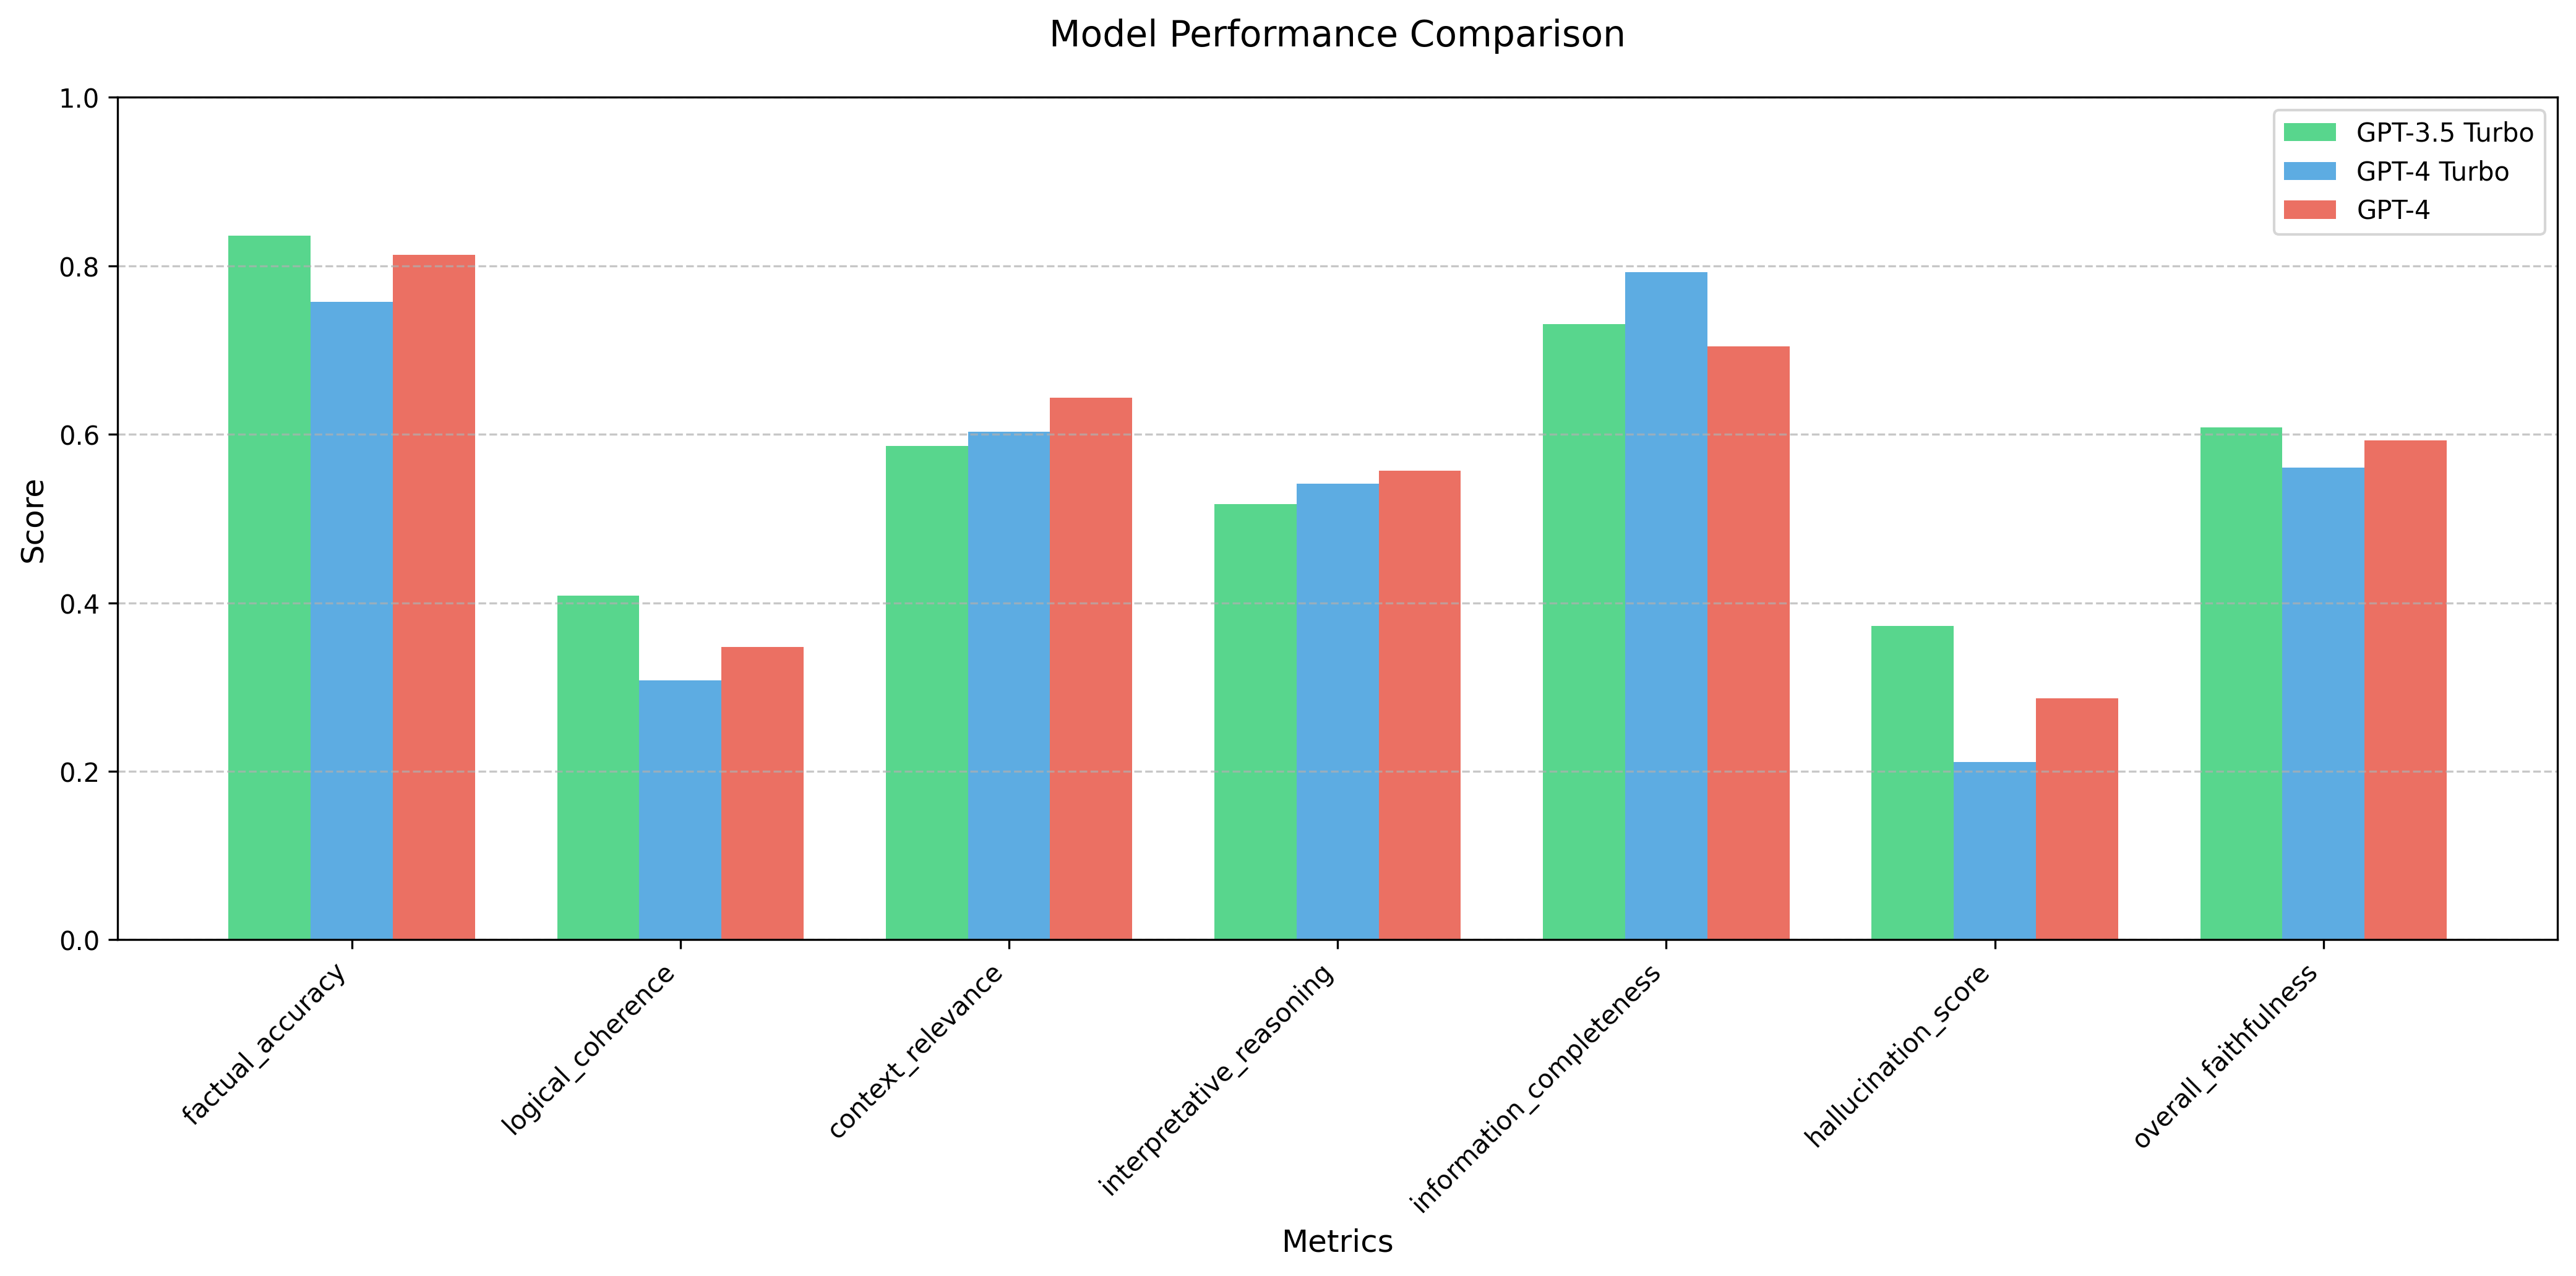
\includegraphics[width=0.8\textwidth]{figures/overall/model_comparison.png}
\caption{Comparative Performance Across Models}
\label{fig:model_comparison}
\end{figure}

The model comparison reveals several interesting patterns:
\begin{itemize}
    \item Factual accuracy remains consistently high across all models (>0.75)
    \item Logical coherence shows the most variation between models
    \item Information completeness demonstrates an inverse relationship with hallucination scores
\end{itemize}

\subsubsection{Overall Metrics Radar Charts}
The radar charts provide a multidimensional view of each model's performance, highlighting their unique characteristics and balance across different metrics.

\begin{figure}[!htbp]
\centering
\begin{subfigure}{0.3\textwidth}
    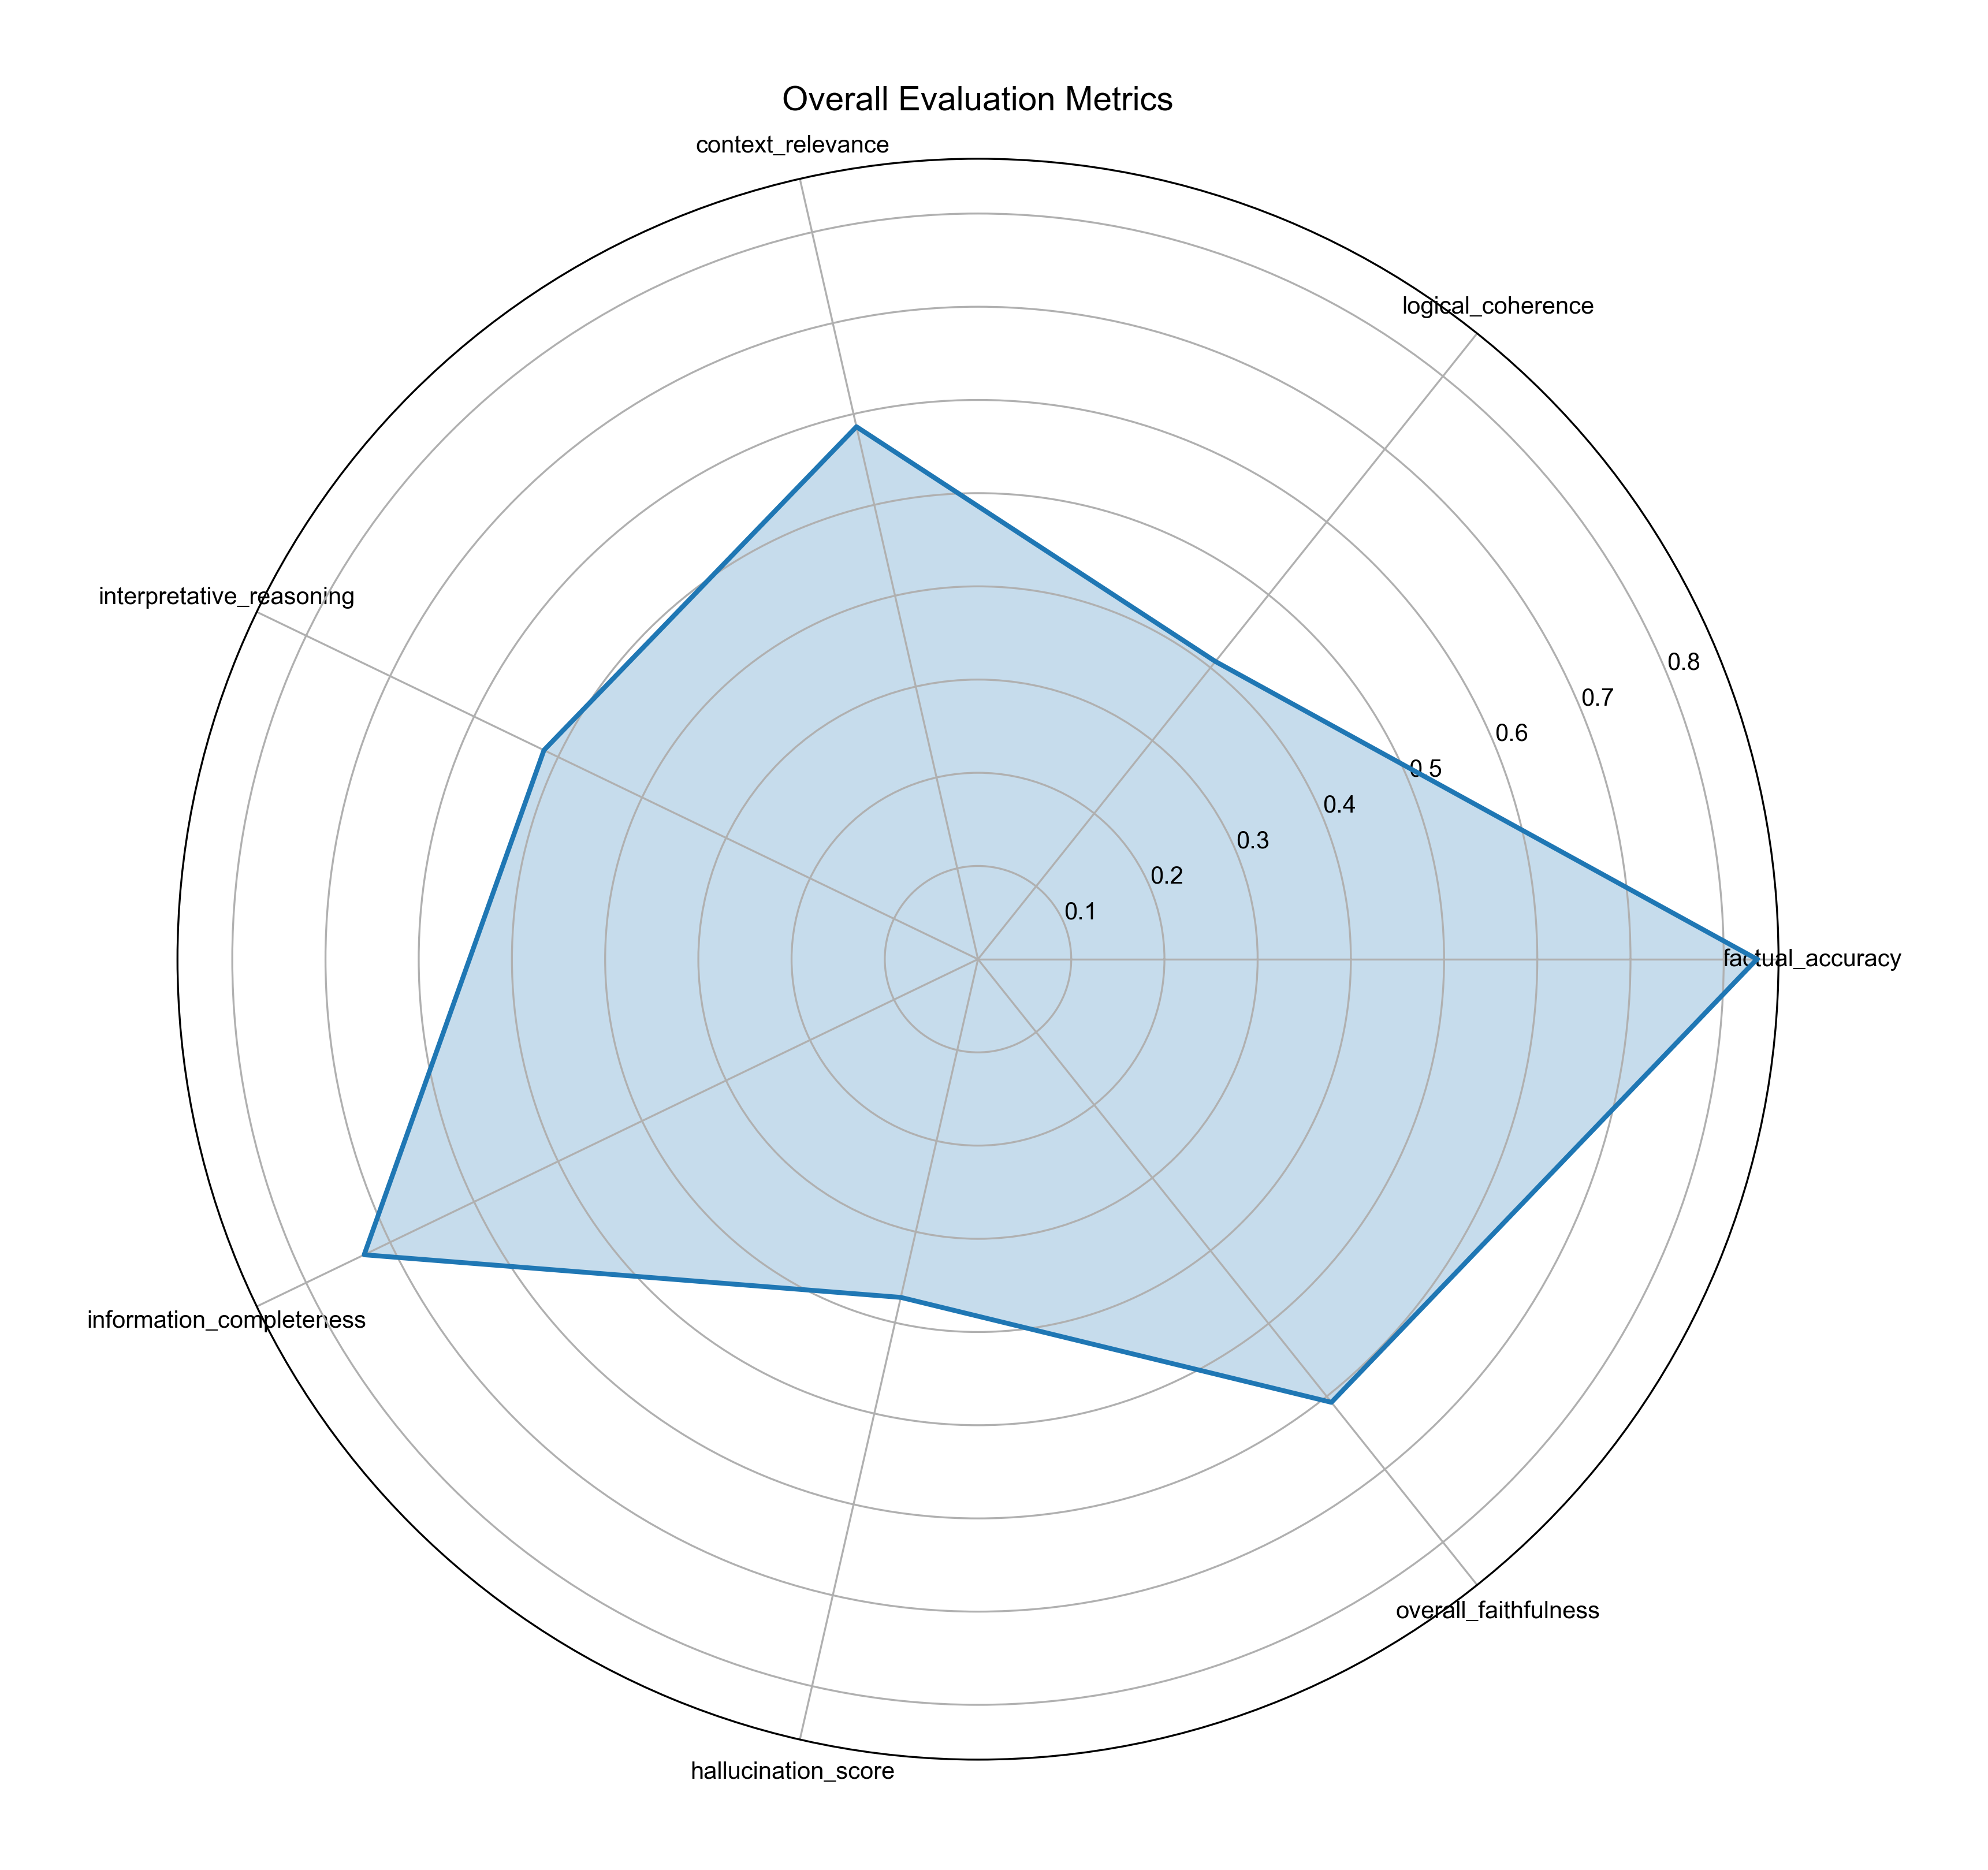
\includegraphics[width=\textwidth]{figures/overall/overall_metrics_radar_gpt-3.5-turbo.png}
    \caption{GPT-3.5-Turbo Metrics}
    \label{fig:overall_metrics_radar_gpt35}
\end{subfigure}
\begin{subfigure}{0.3\textwidth}
    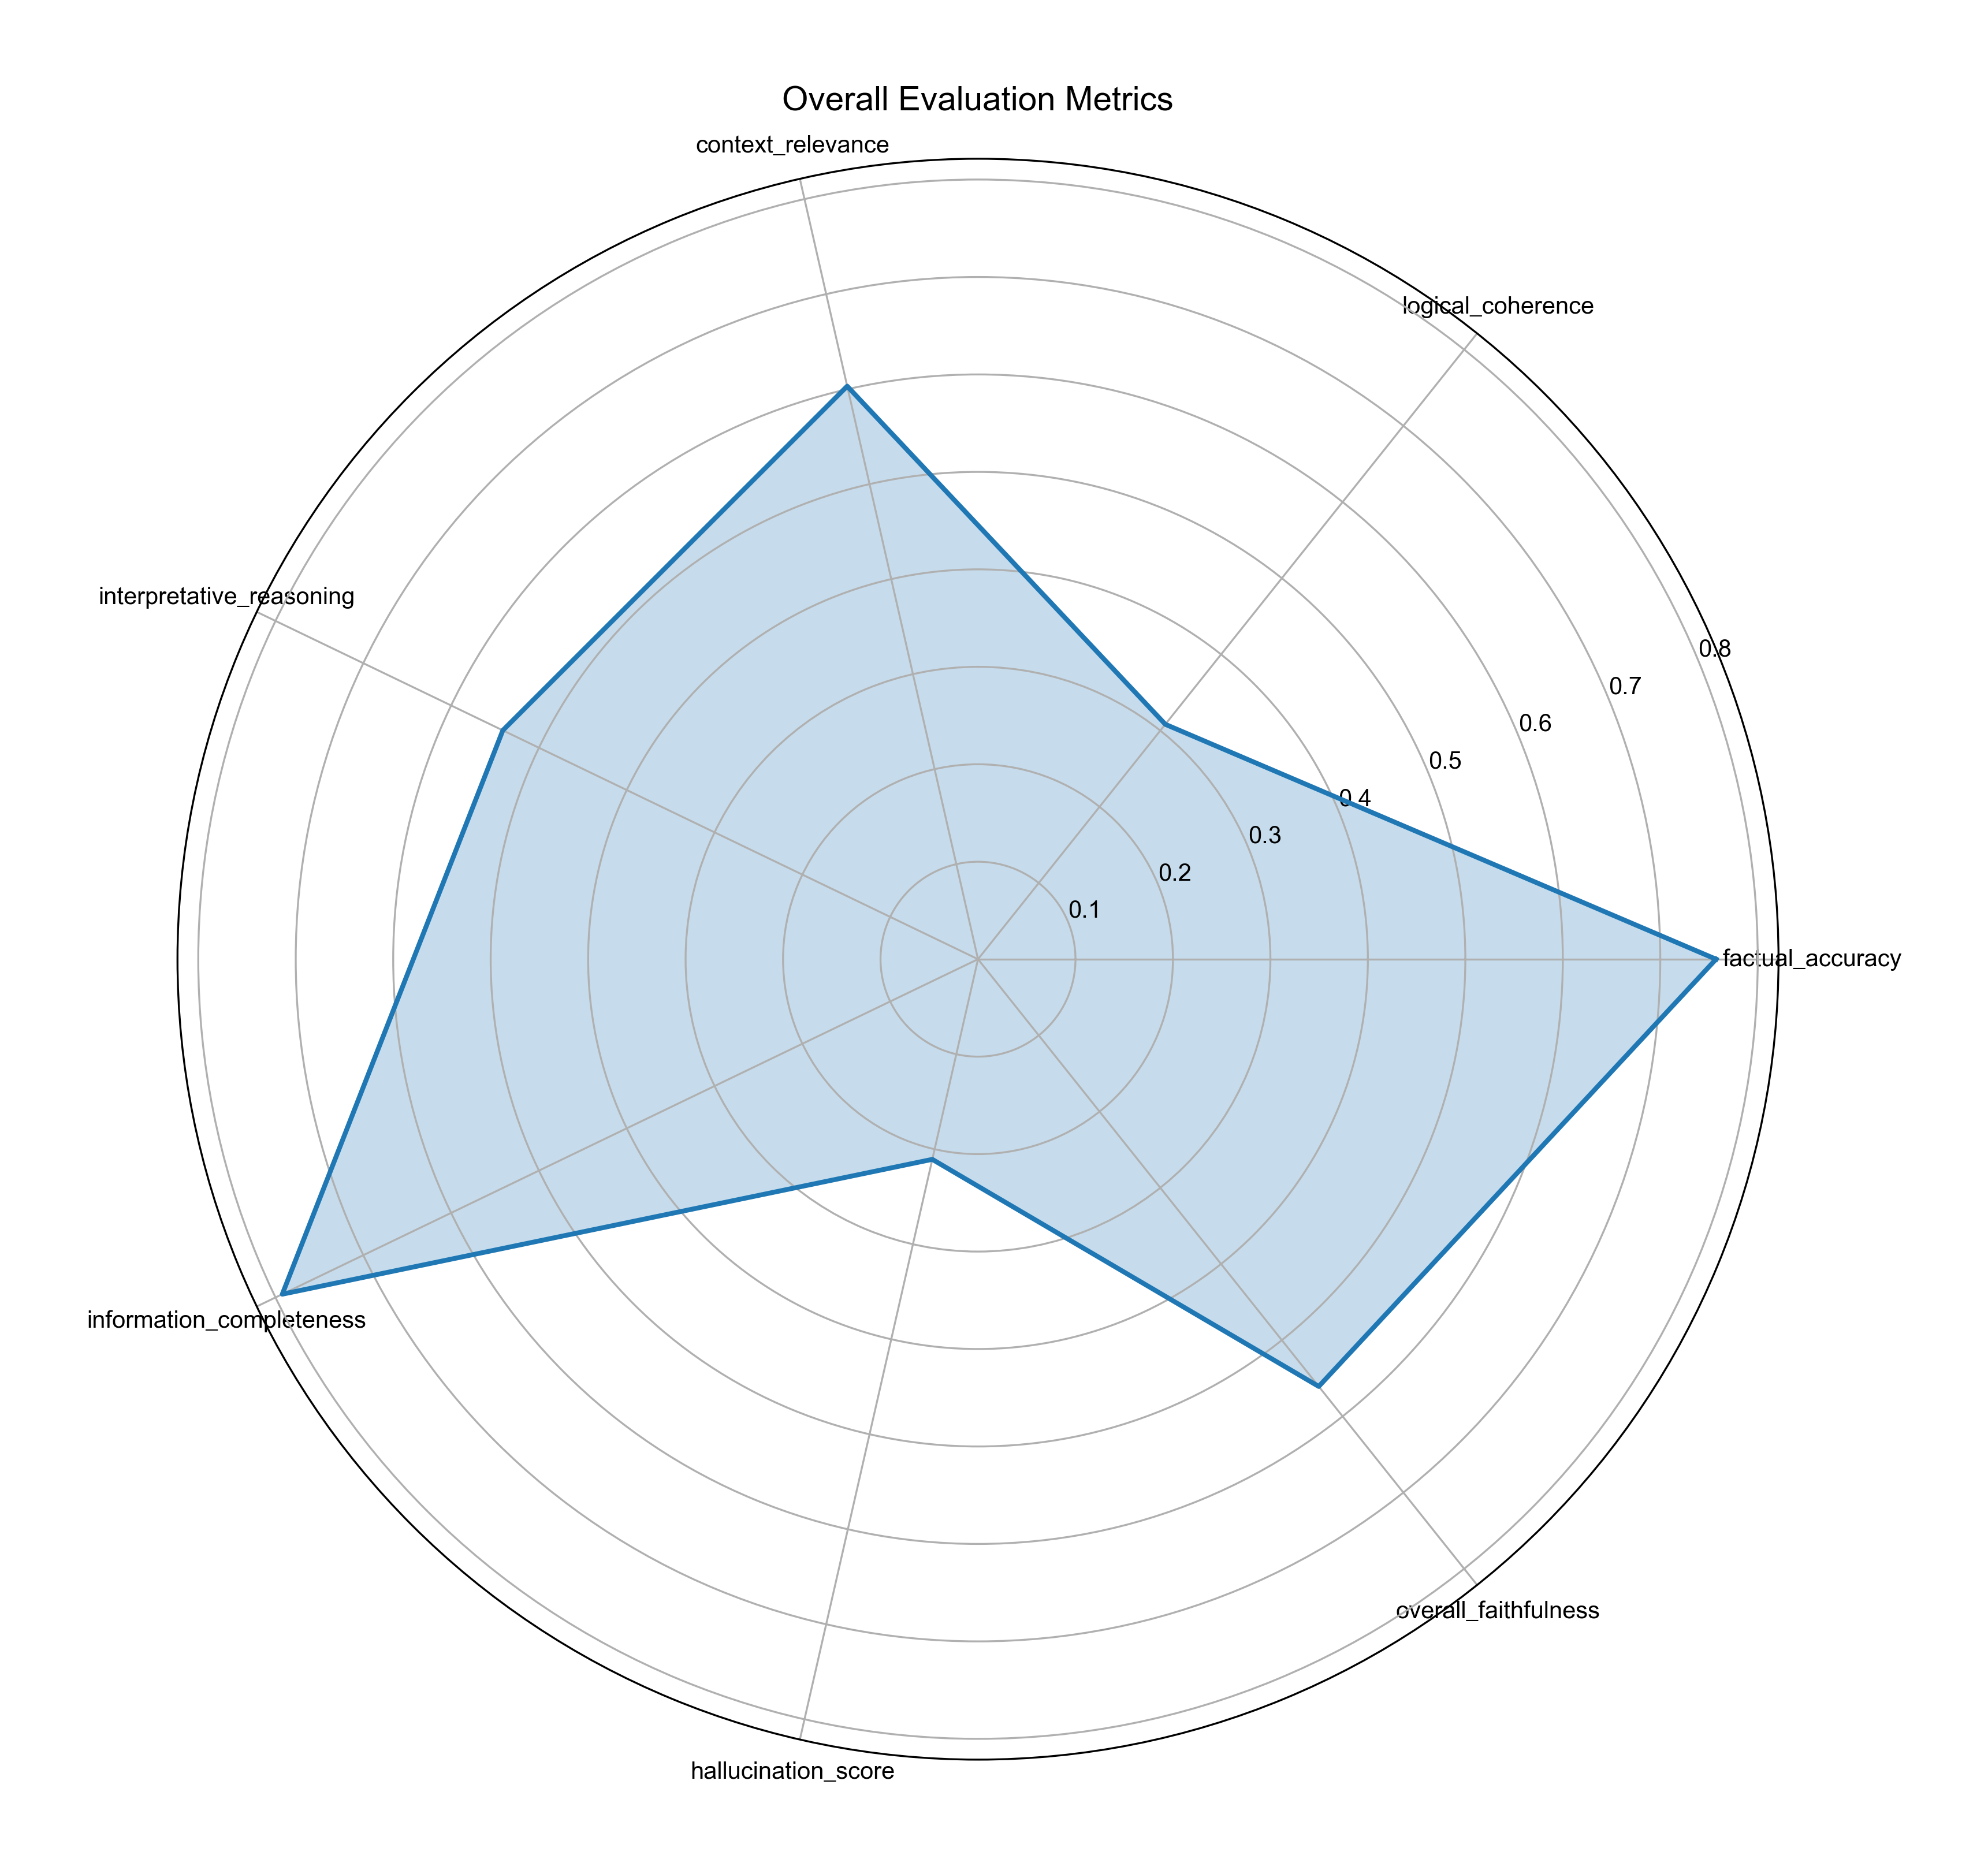
\includegraphics[width=\textwidth]{figures/overall/overall_metrics_radar_gpt-4-turbo.png}
    \caption{GPT-4-Turbo Metrics}
    \label{fig:overall_metrics_radar_gpt4t}
\end{subfigure}
\begin{subfigure}{0.3\textwidth}
    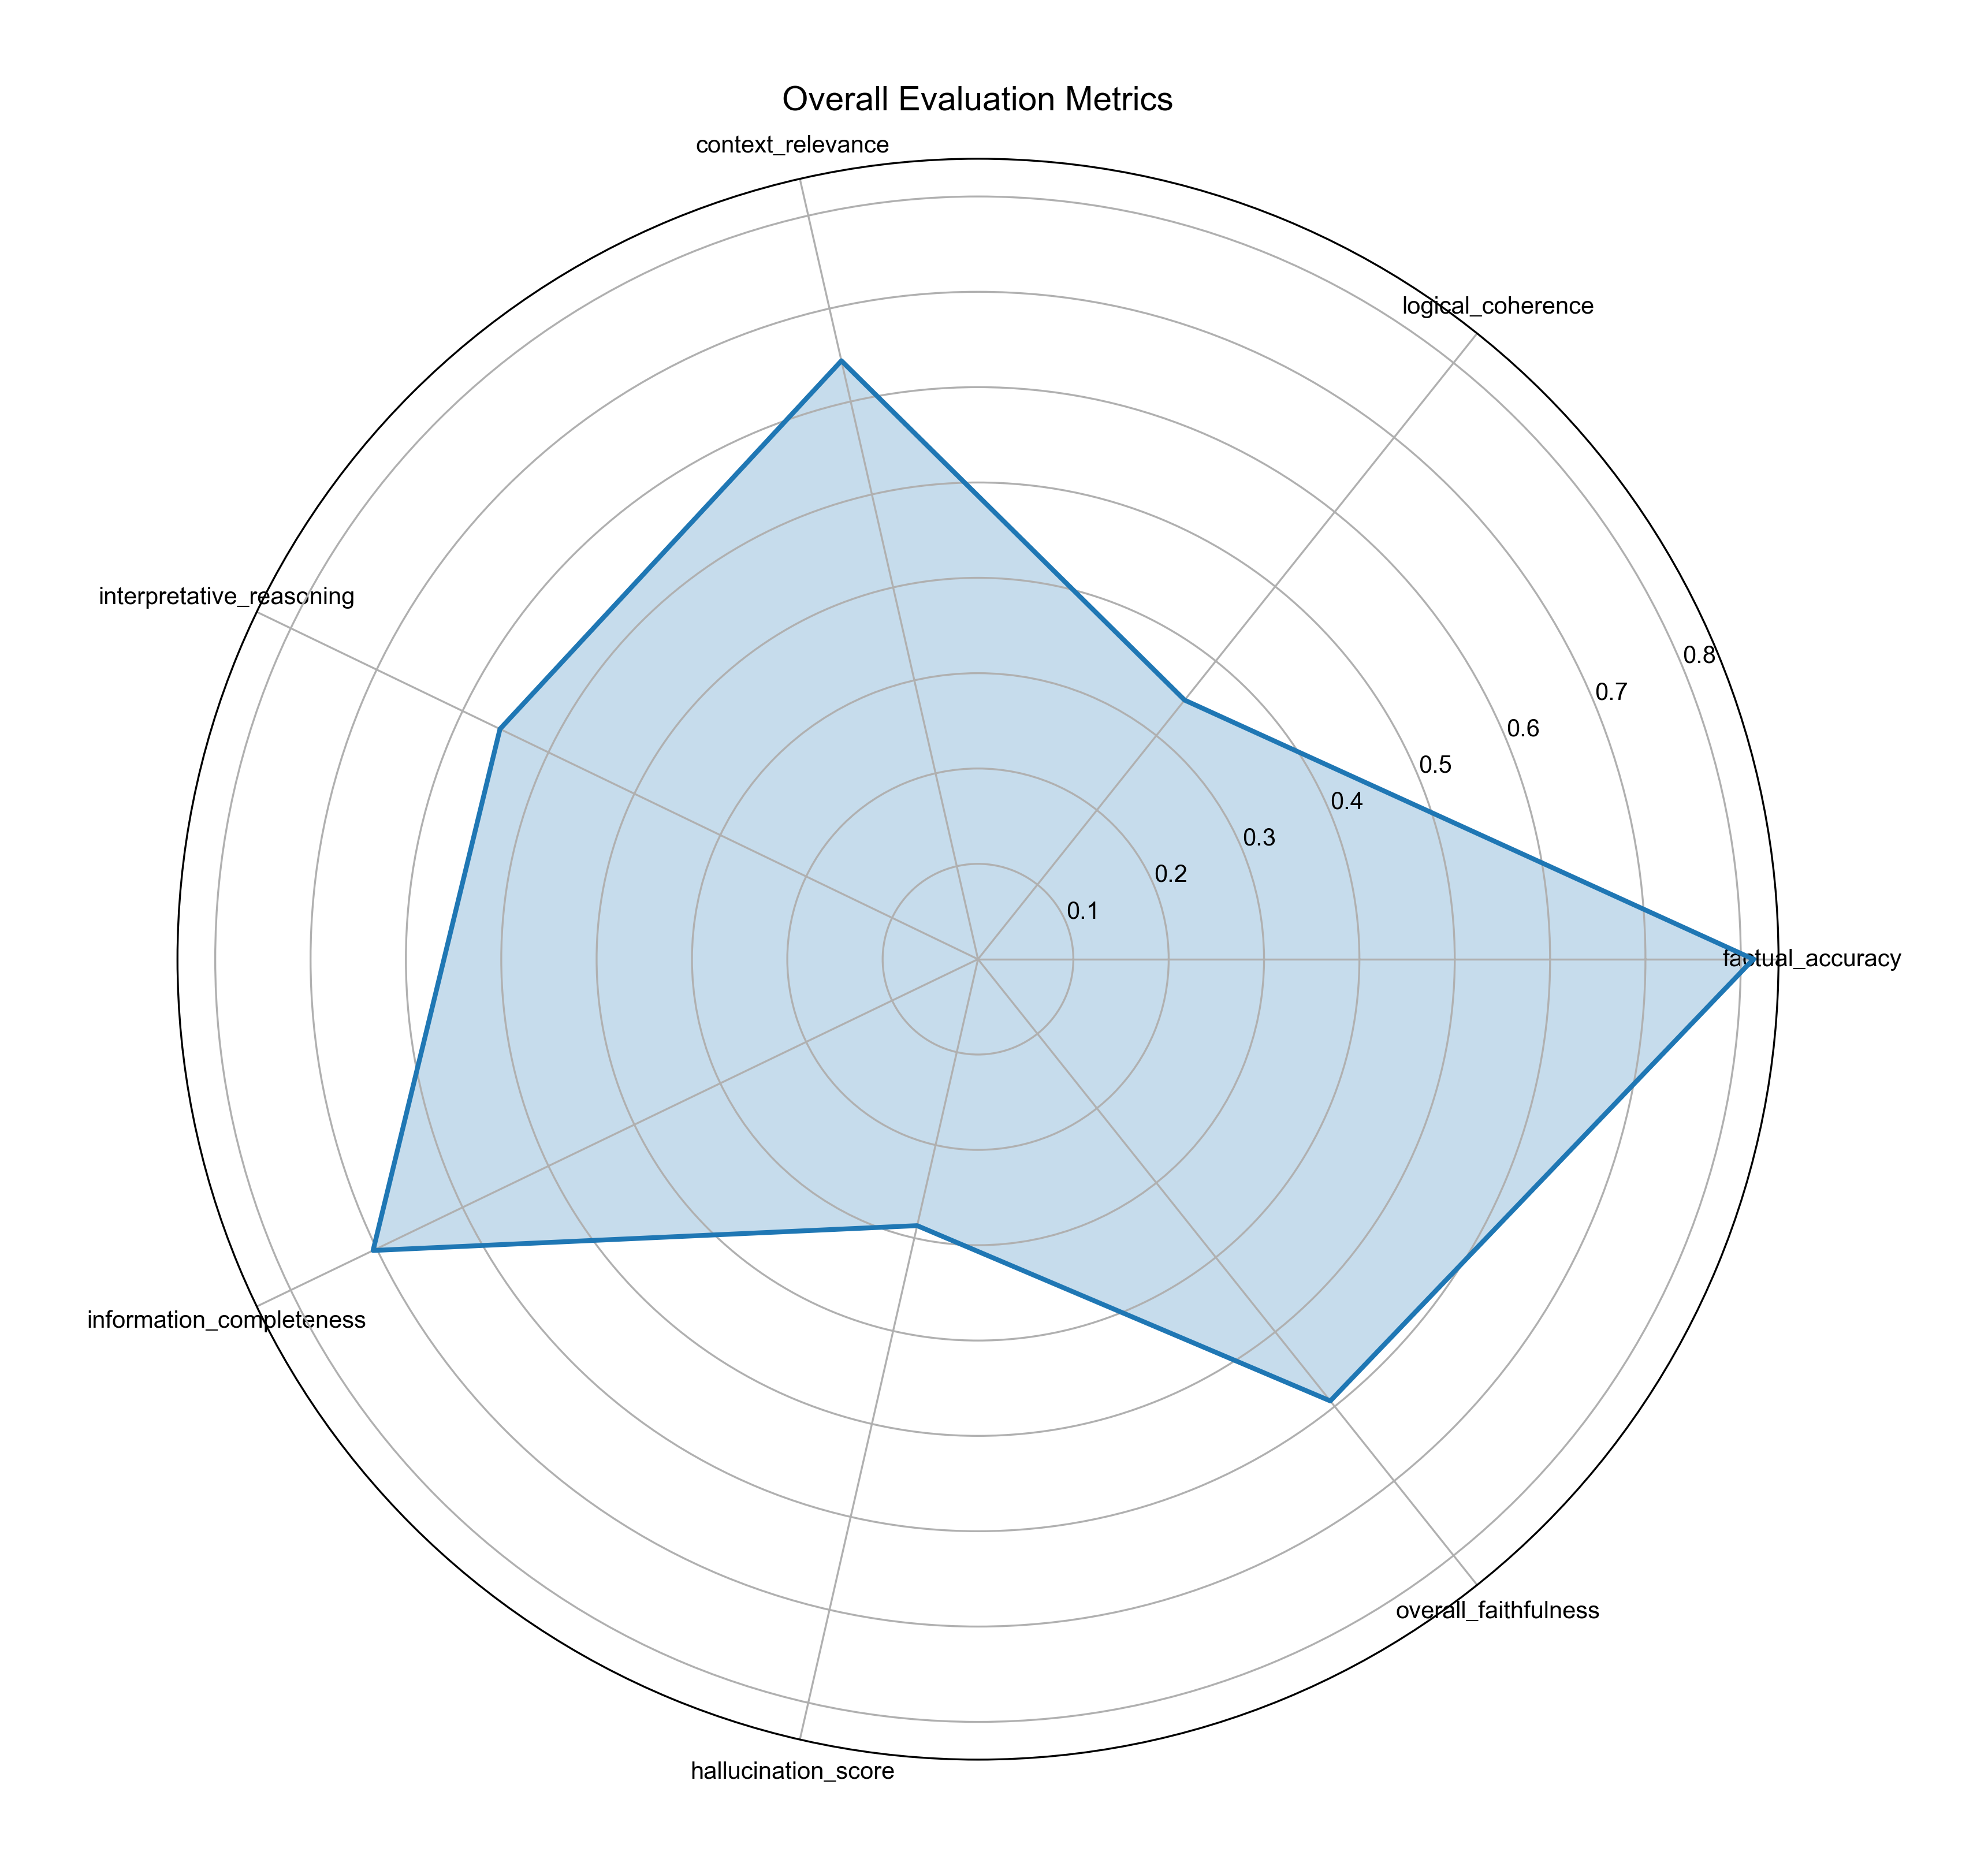
\includegraphics[width=\textwidth]{figures/overall/overall_metrics_radar_gpt-4.png}
    \caption{GPT-4 Metrics}
    \label{fig:overall_metrics_radar_gpt4}
\end{subfigure}
\caption{Overall Metrics Radar Charts by Model}
\label{fig:overall_metrics_radar}
\end{figure}

\textbf{Radar Chart Analysis}:
\begin{itemize}
    \item Each model exhibits distinct patterns in their metric distribution
    \item GPT-3.5-Turbo shows more balanced performance across metrics
    \item GPT-4 variants demonstrate stronger performance in specific areas
\end{itemize}

\subsubsection{Metrics Trend Analysis}
The trend analysis reveals the evolution of different metrics across various evaluation scenarios for each model, providing insights into their performance stability and patterns.

\begin{figure}[!htbp]
\centering
\begin{subfigure}{0.3\textwidth}
    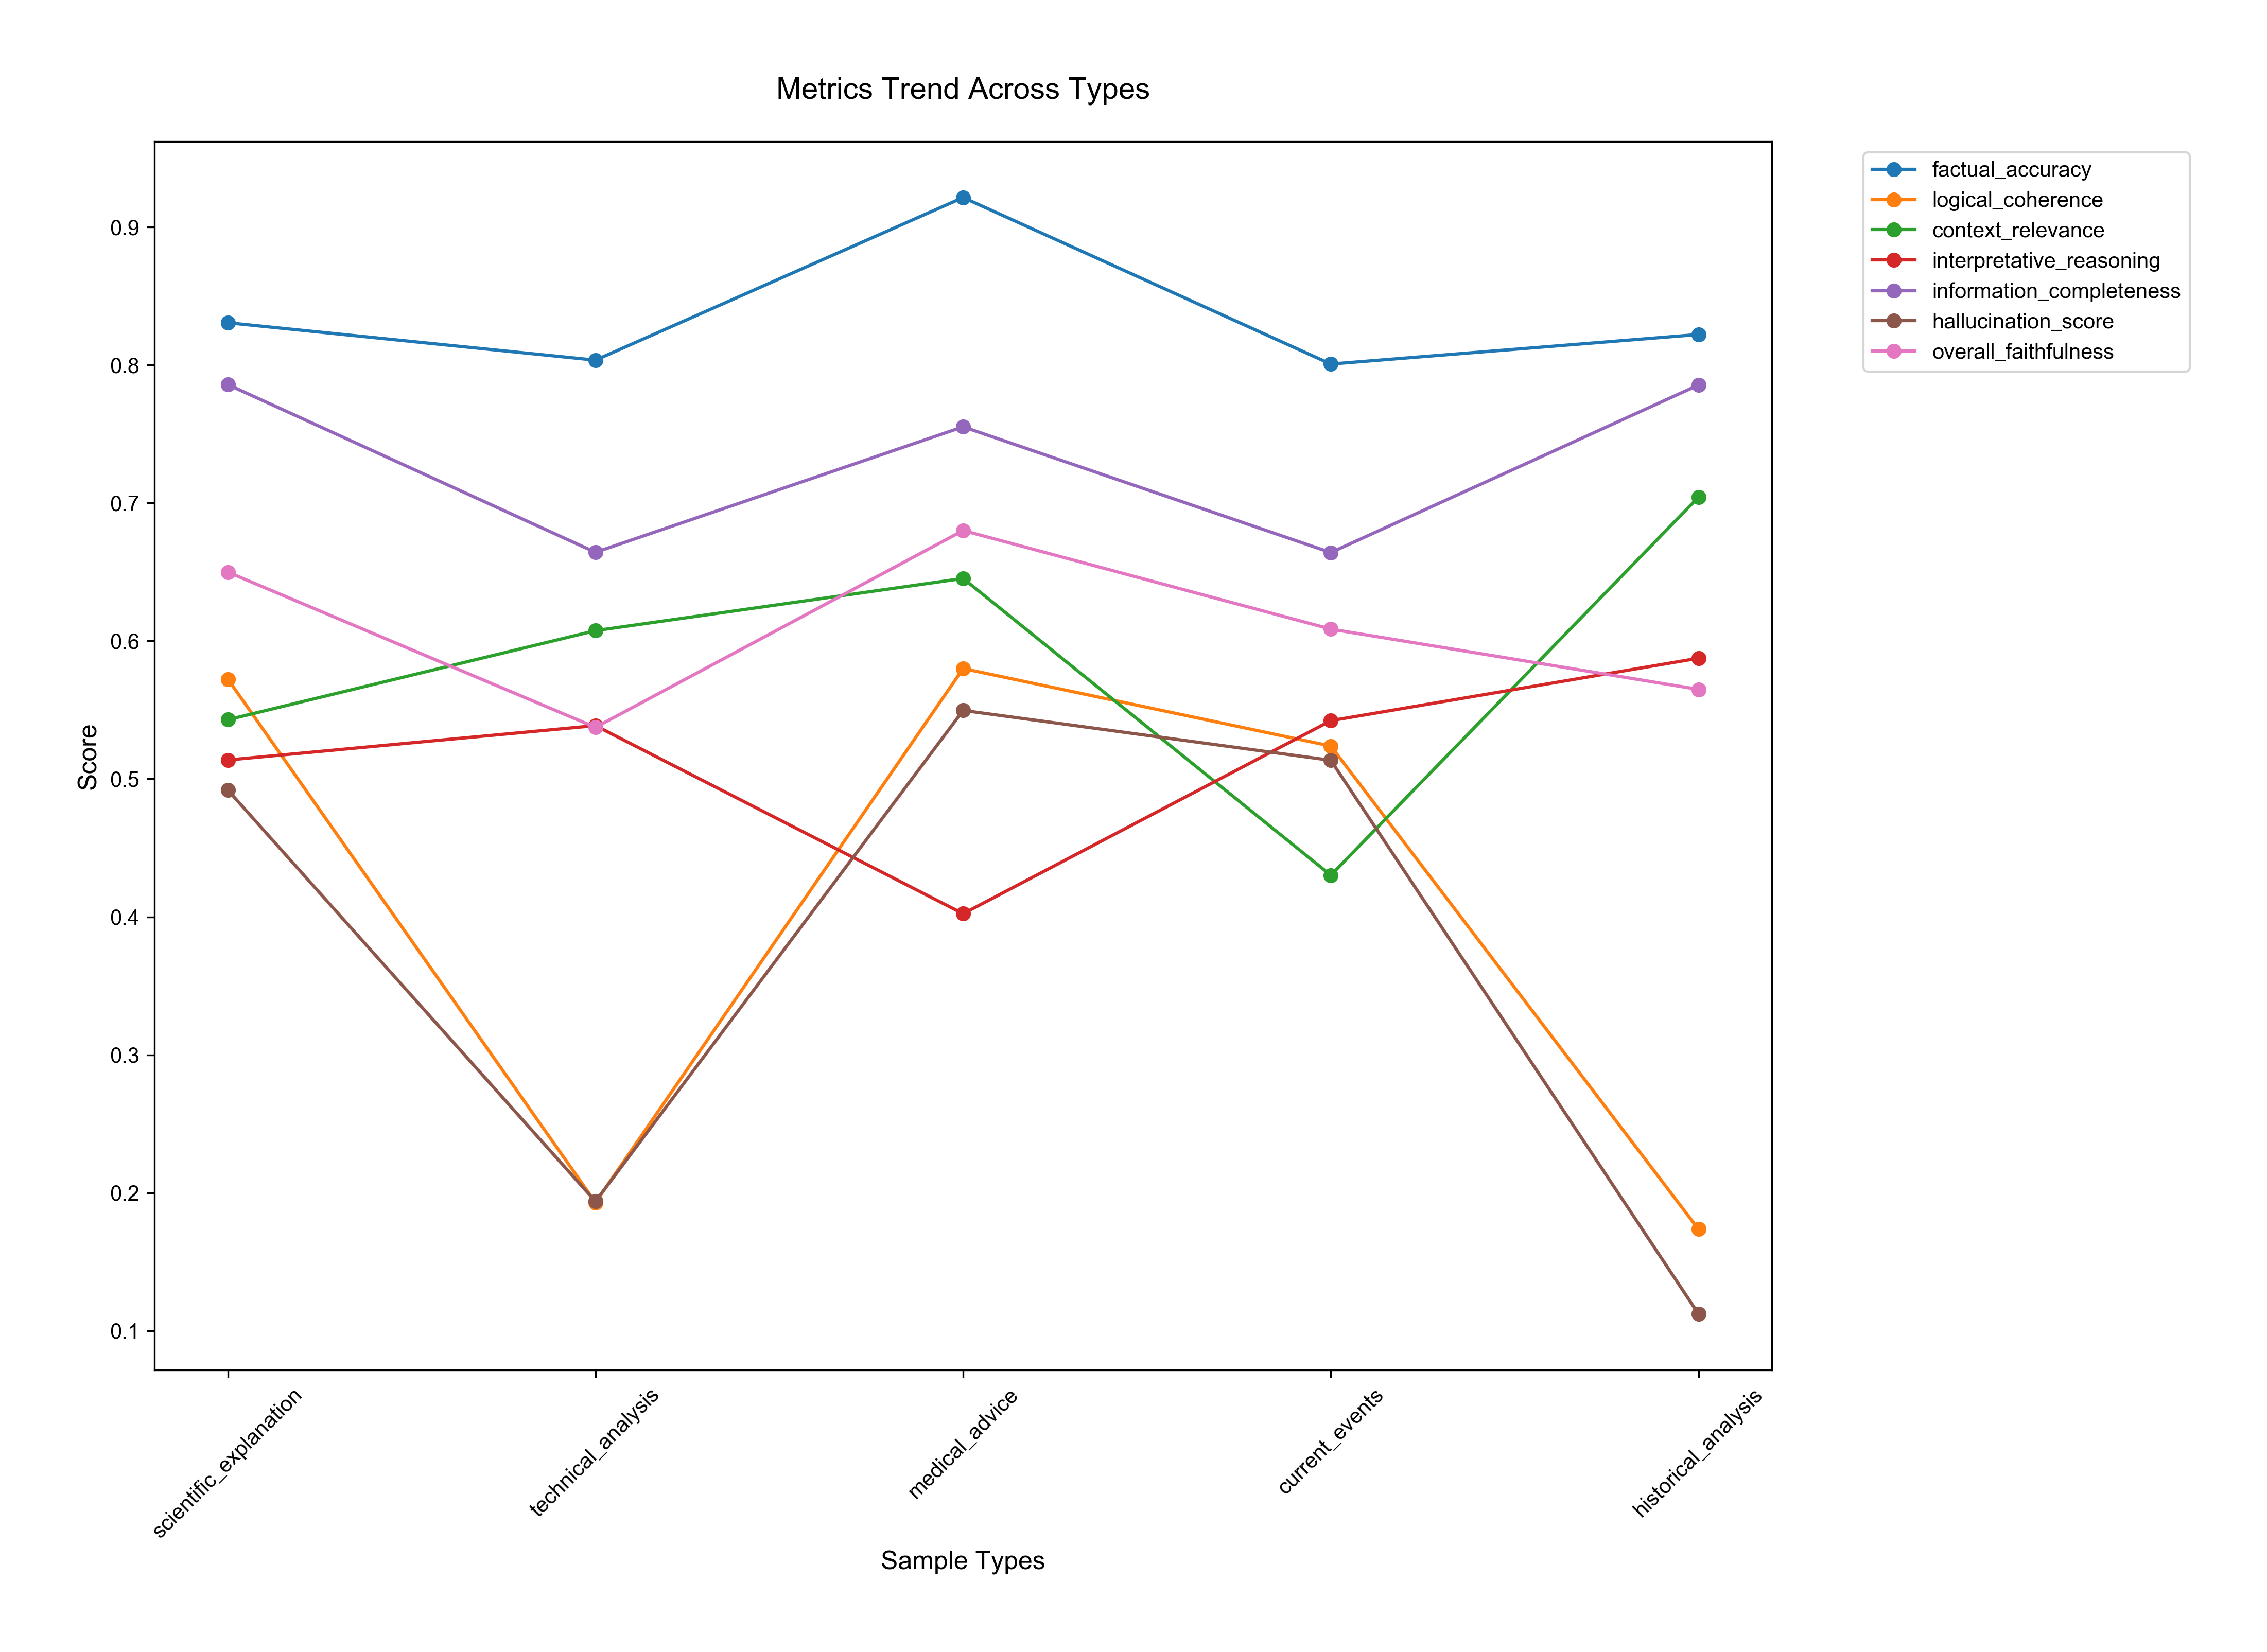
\includegraphics[width=\textwidth]{figures/overall/metrics_trend_gpt-3.5-turbo.png}
    \caption{GPT-3.5-Turbo Trends}
    \label{fig:metrics_trend_gpt35}
\end{subfigure}
\begin{subfigure}{0.3\textwidth}
    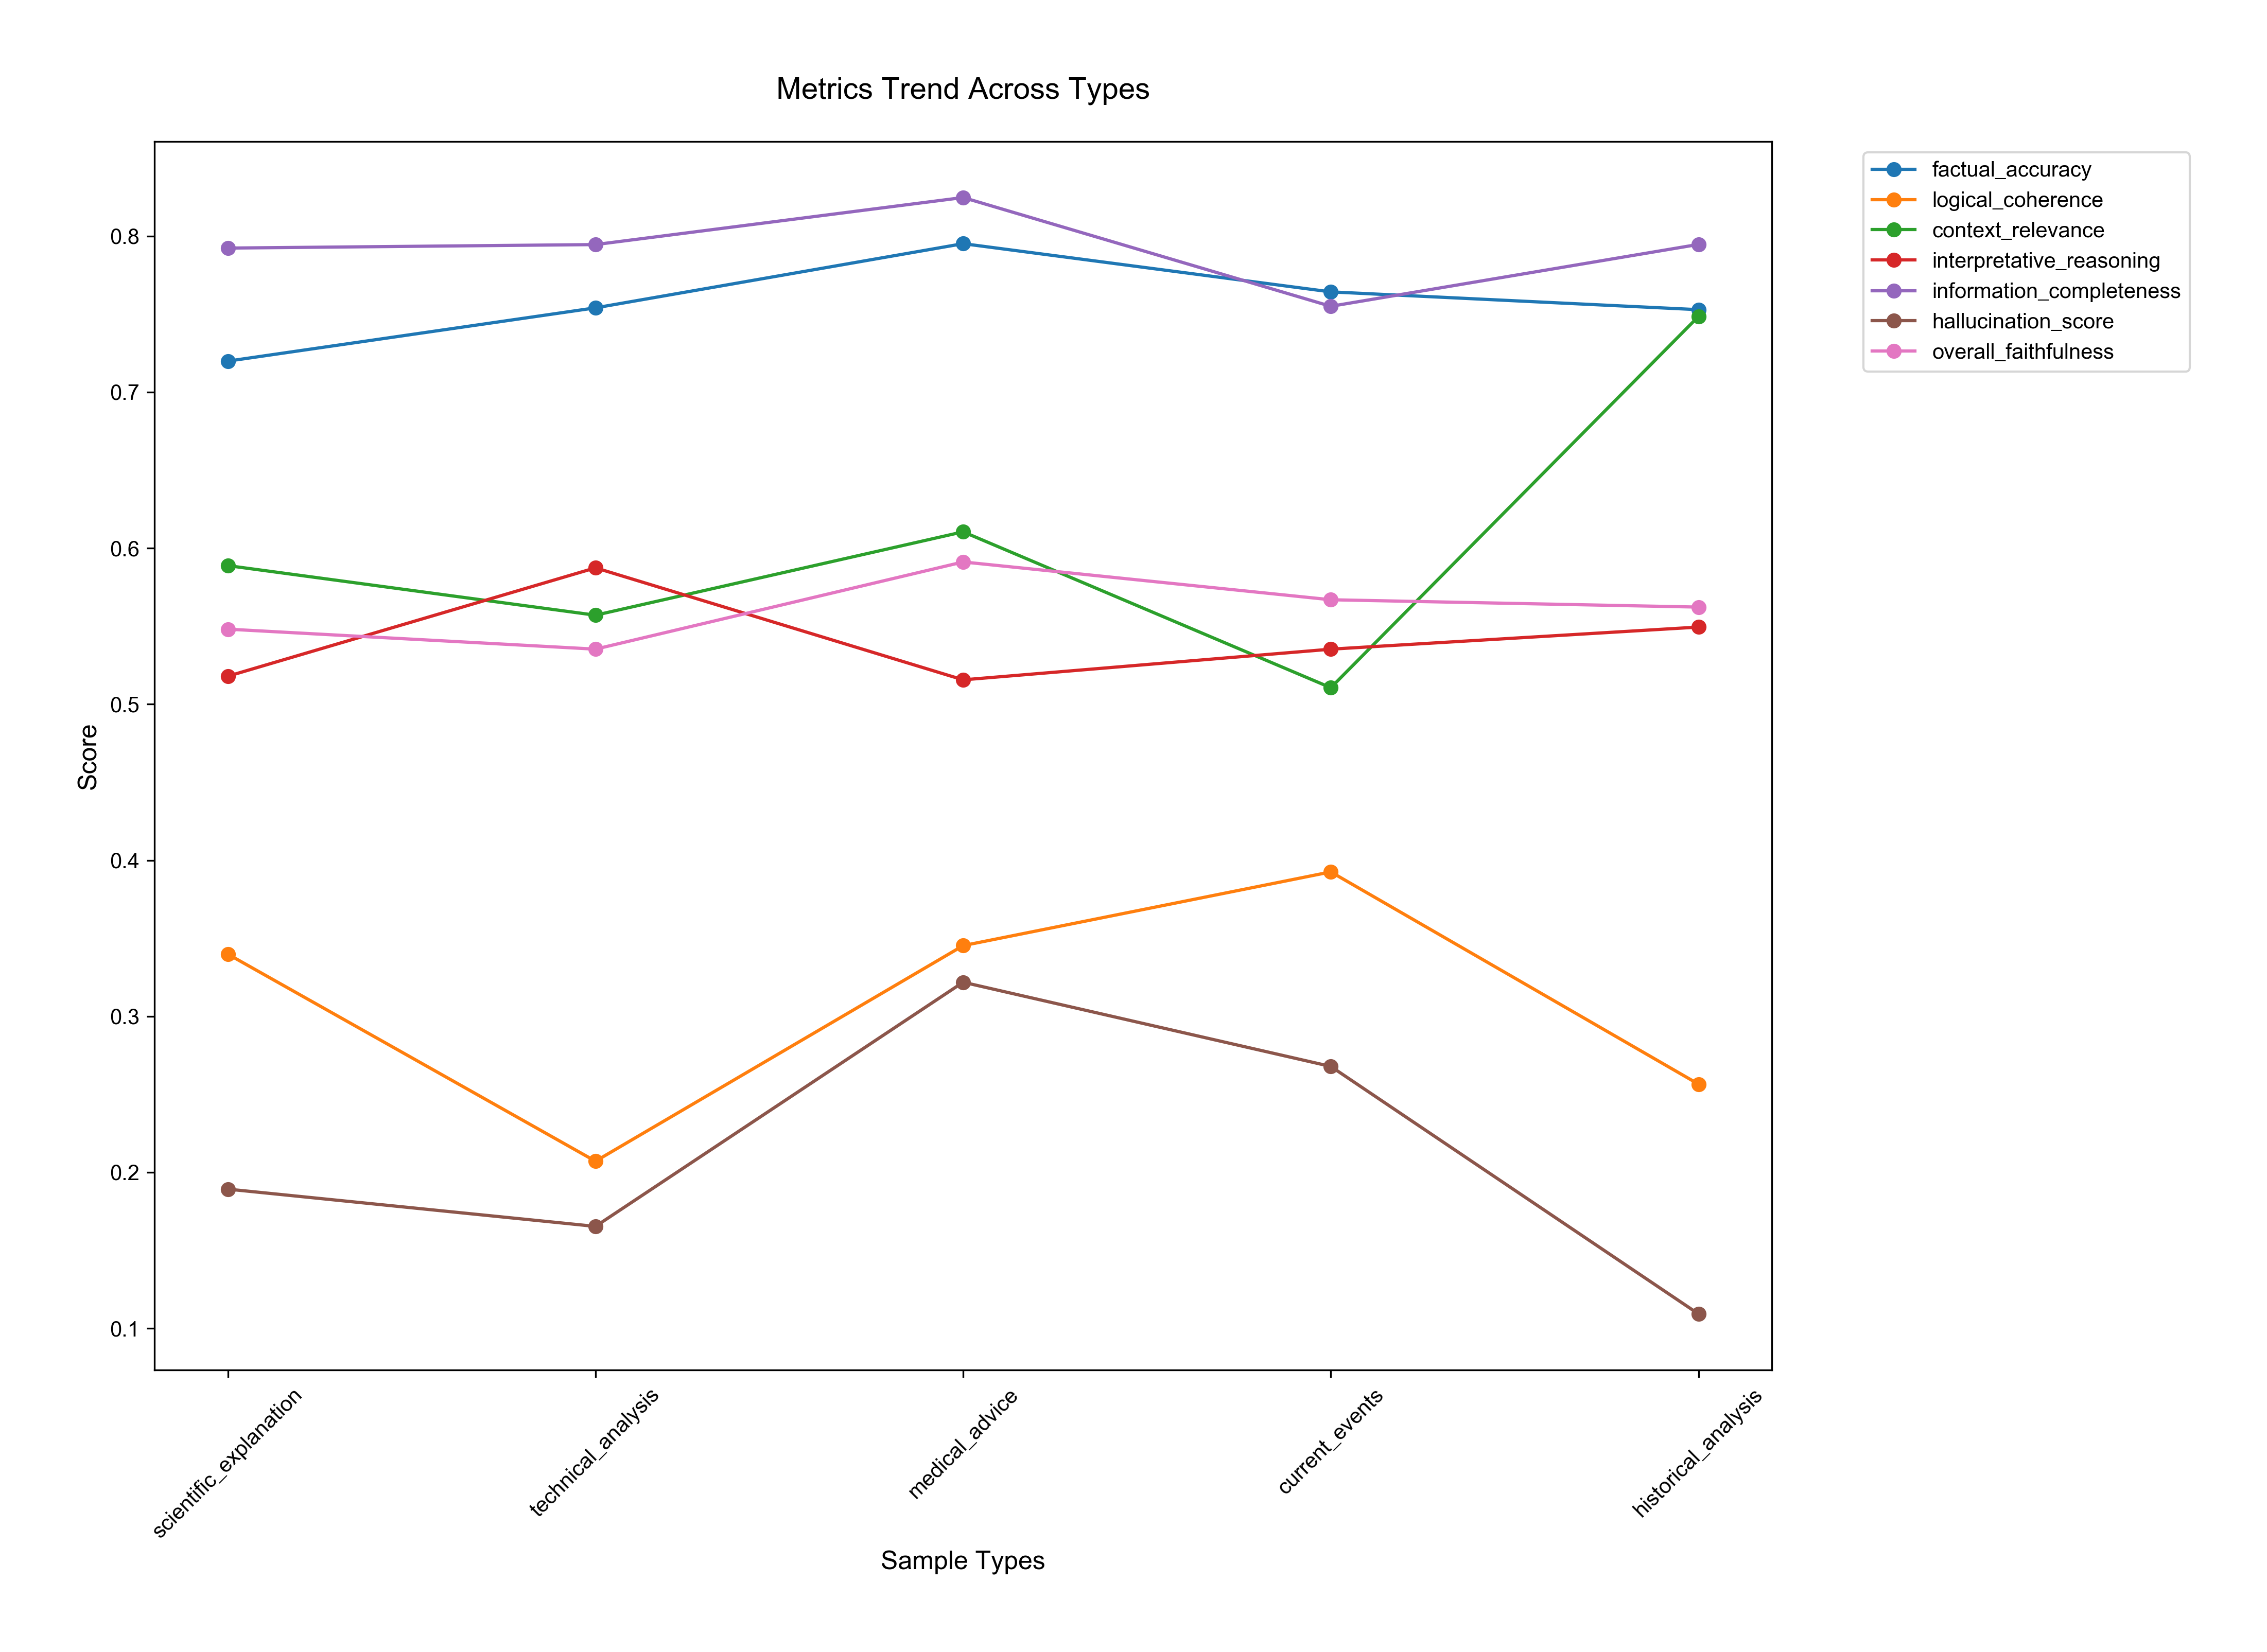
\includegraphics[width=\textwidth]{figures/overall/metrics_trend_gpt-4-turbo.png}
    \caption{GPT-4-Turbo Trends}
    \label{fig:metrics_trend_gpt4t}
\end{subfigure}
\begin{subfigure}{0.3\textwidth}
    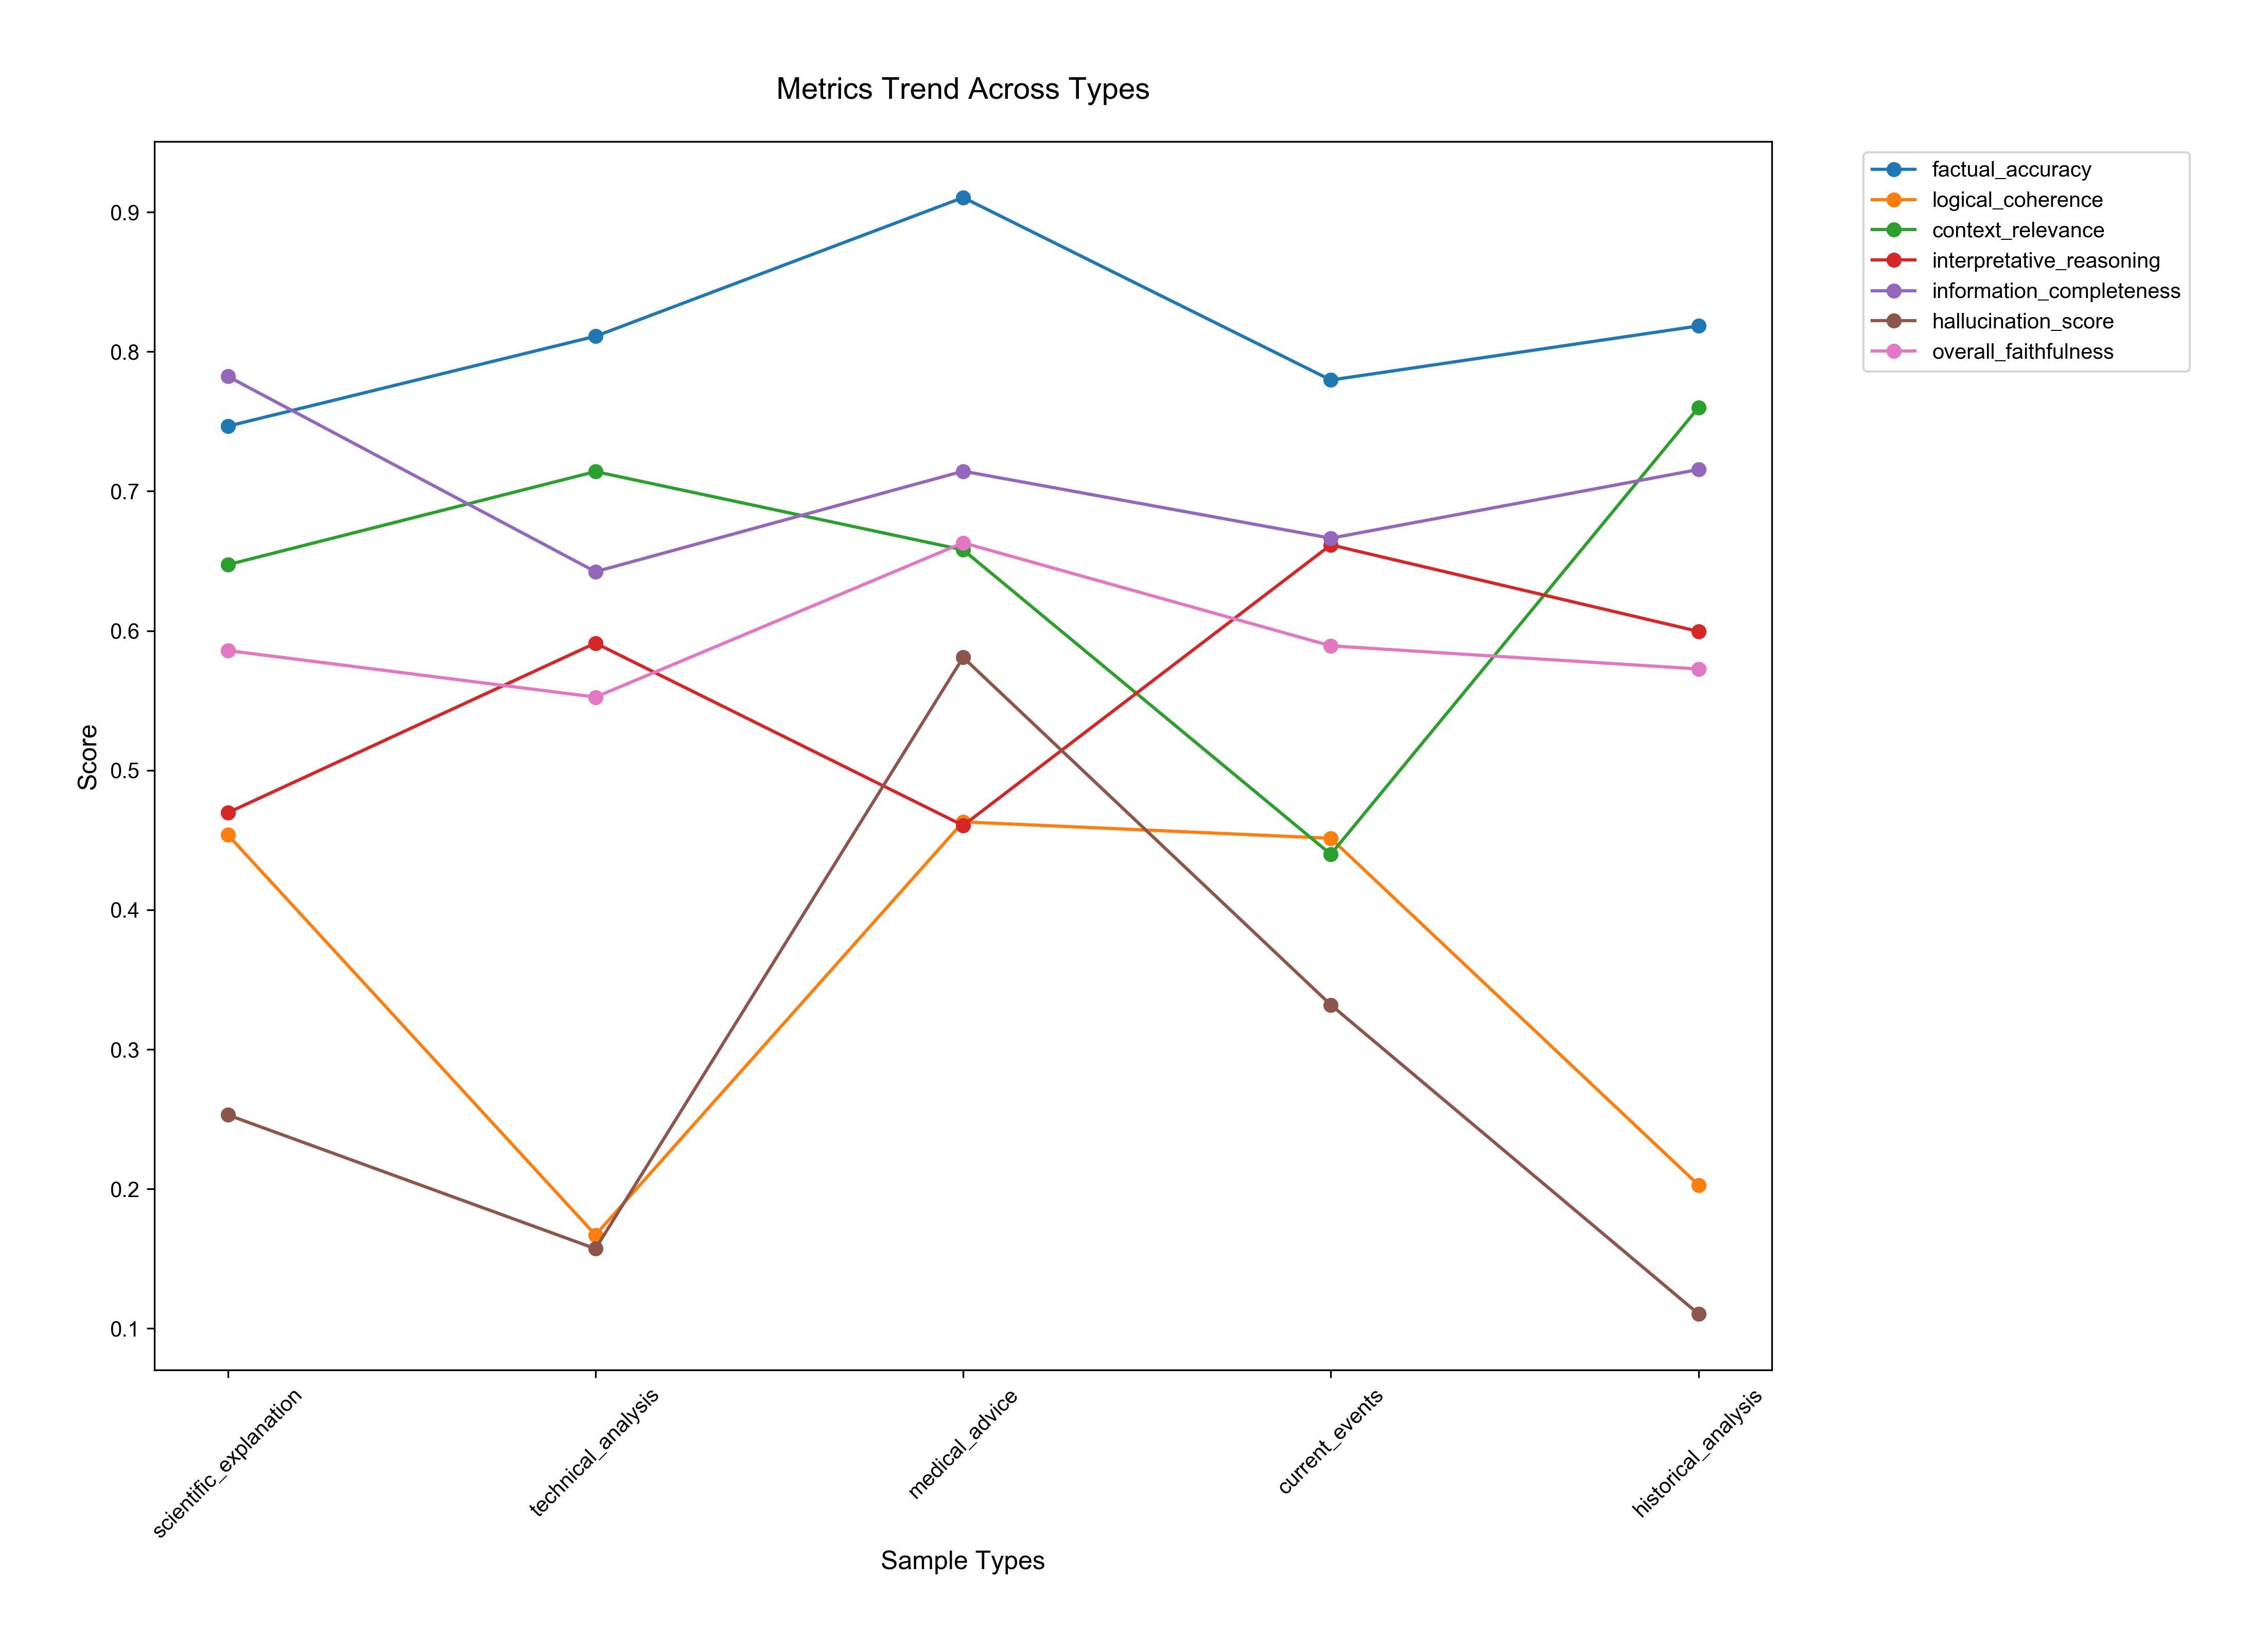
\includegraphics[width=\textwidth]{figures/overall/metrics_trend_gpt-4.png}
    \caption{GPT-4 Trends}
    \label{fig:metrics_trend_gpt4}
\end{subfigure}
\caption{Metrics Trend Analysis by Model}
\label{fig:metrics_trends}
\end{figure}

\textbf{Key Trend Observations}:
\begin{itemize}
    \item \textbf{Factual Accuracy}: Shows consistent high performance across all models, with minor fluctuations
    \item \textbf{Logical Coherence}: Exhibits the most variability, particularly in complex scenarios
    \item \textbf{Context Relevance}: Demonstrates steady improvement as models process more context
    \item \textbf{Hallucination Scores}: Show decreasing trends, indicating better control over fabricated information
\end{itemize}

\subsection{Type-Specific Evaluation Results}

\subsubsection{Scientific Explanation}
The evaluation of scientific explanations focuses on the models' ability to accurately convey complex scientific concepts while maintaining factual integrity.

\begin{table}[!htbp]
\centering
\setlength{\tabcolsep}{4pt}  % Reduce table column spacing
\caption{Scientific Explanation Metrics}
\label{tab:results_scientific_metrics}
\begin{tabular}{|l|c|c|c|c|c|c|c|}
\hline
\textbf{Model} & \textbf{Fact.} & \textbf{Logic} & \textbf{Context} & \textbf{Interp.} 
& \textbf{Info.} & \textbf{Hall.} & \textbf{Overall} \\
\hline
GPT-3.5-Turbo & 0.8306 & 0.5723 & 0.5429 & 0.5137 & 0.7858 & 0.4919 & 0.6499 \\
GPT-4-Turbo & 0.7199 & 0.3398 & 0.5888 & 0.5179 & 0.7923 & 0.1892 & 0.5481 \\
GPT-4 & 0.7466 & 0.4538 & 0.6473 & 0.4696 & 0.7823 & 0.2530 & 0.5858 \\
\hline
\end{tabular}
\end{table}

\begin{figure}[!htbp]
\centering
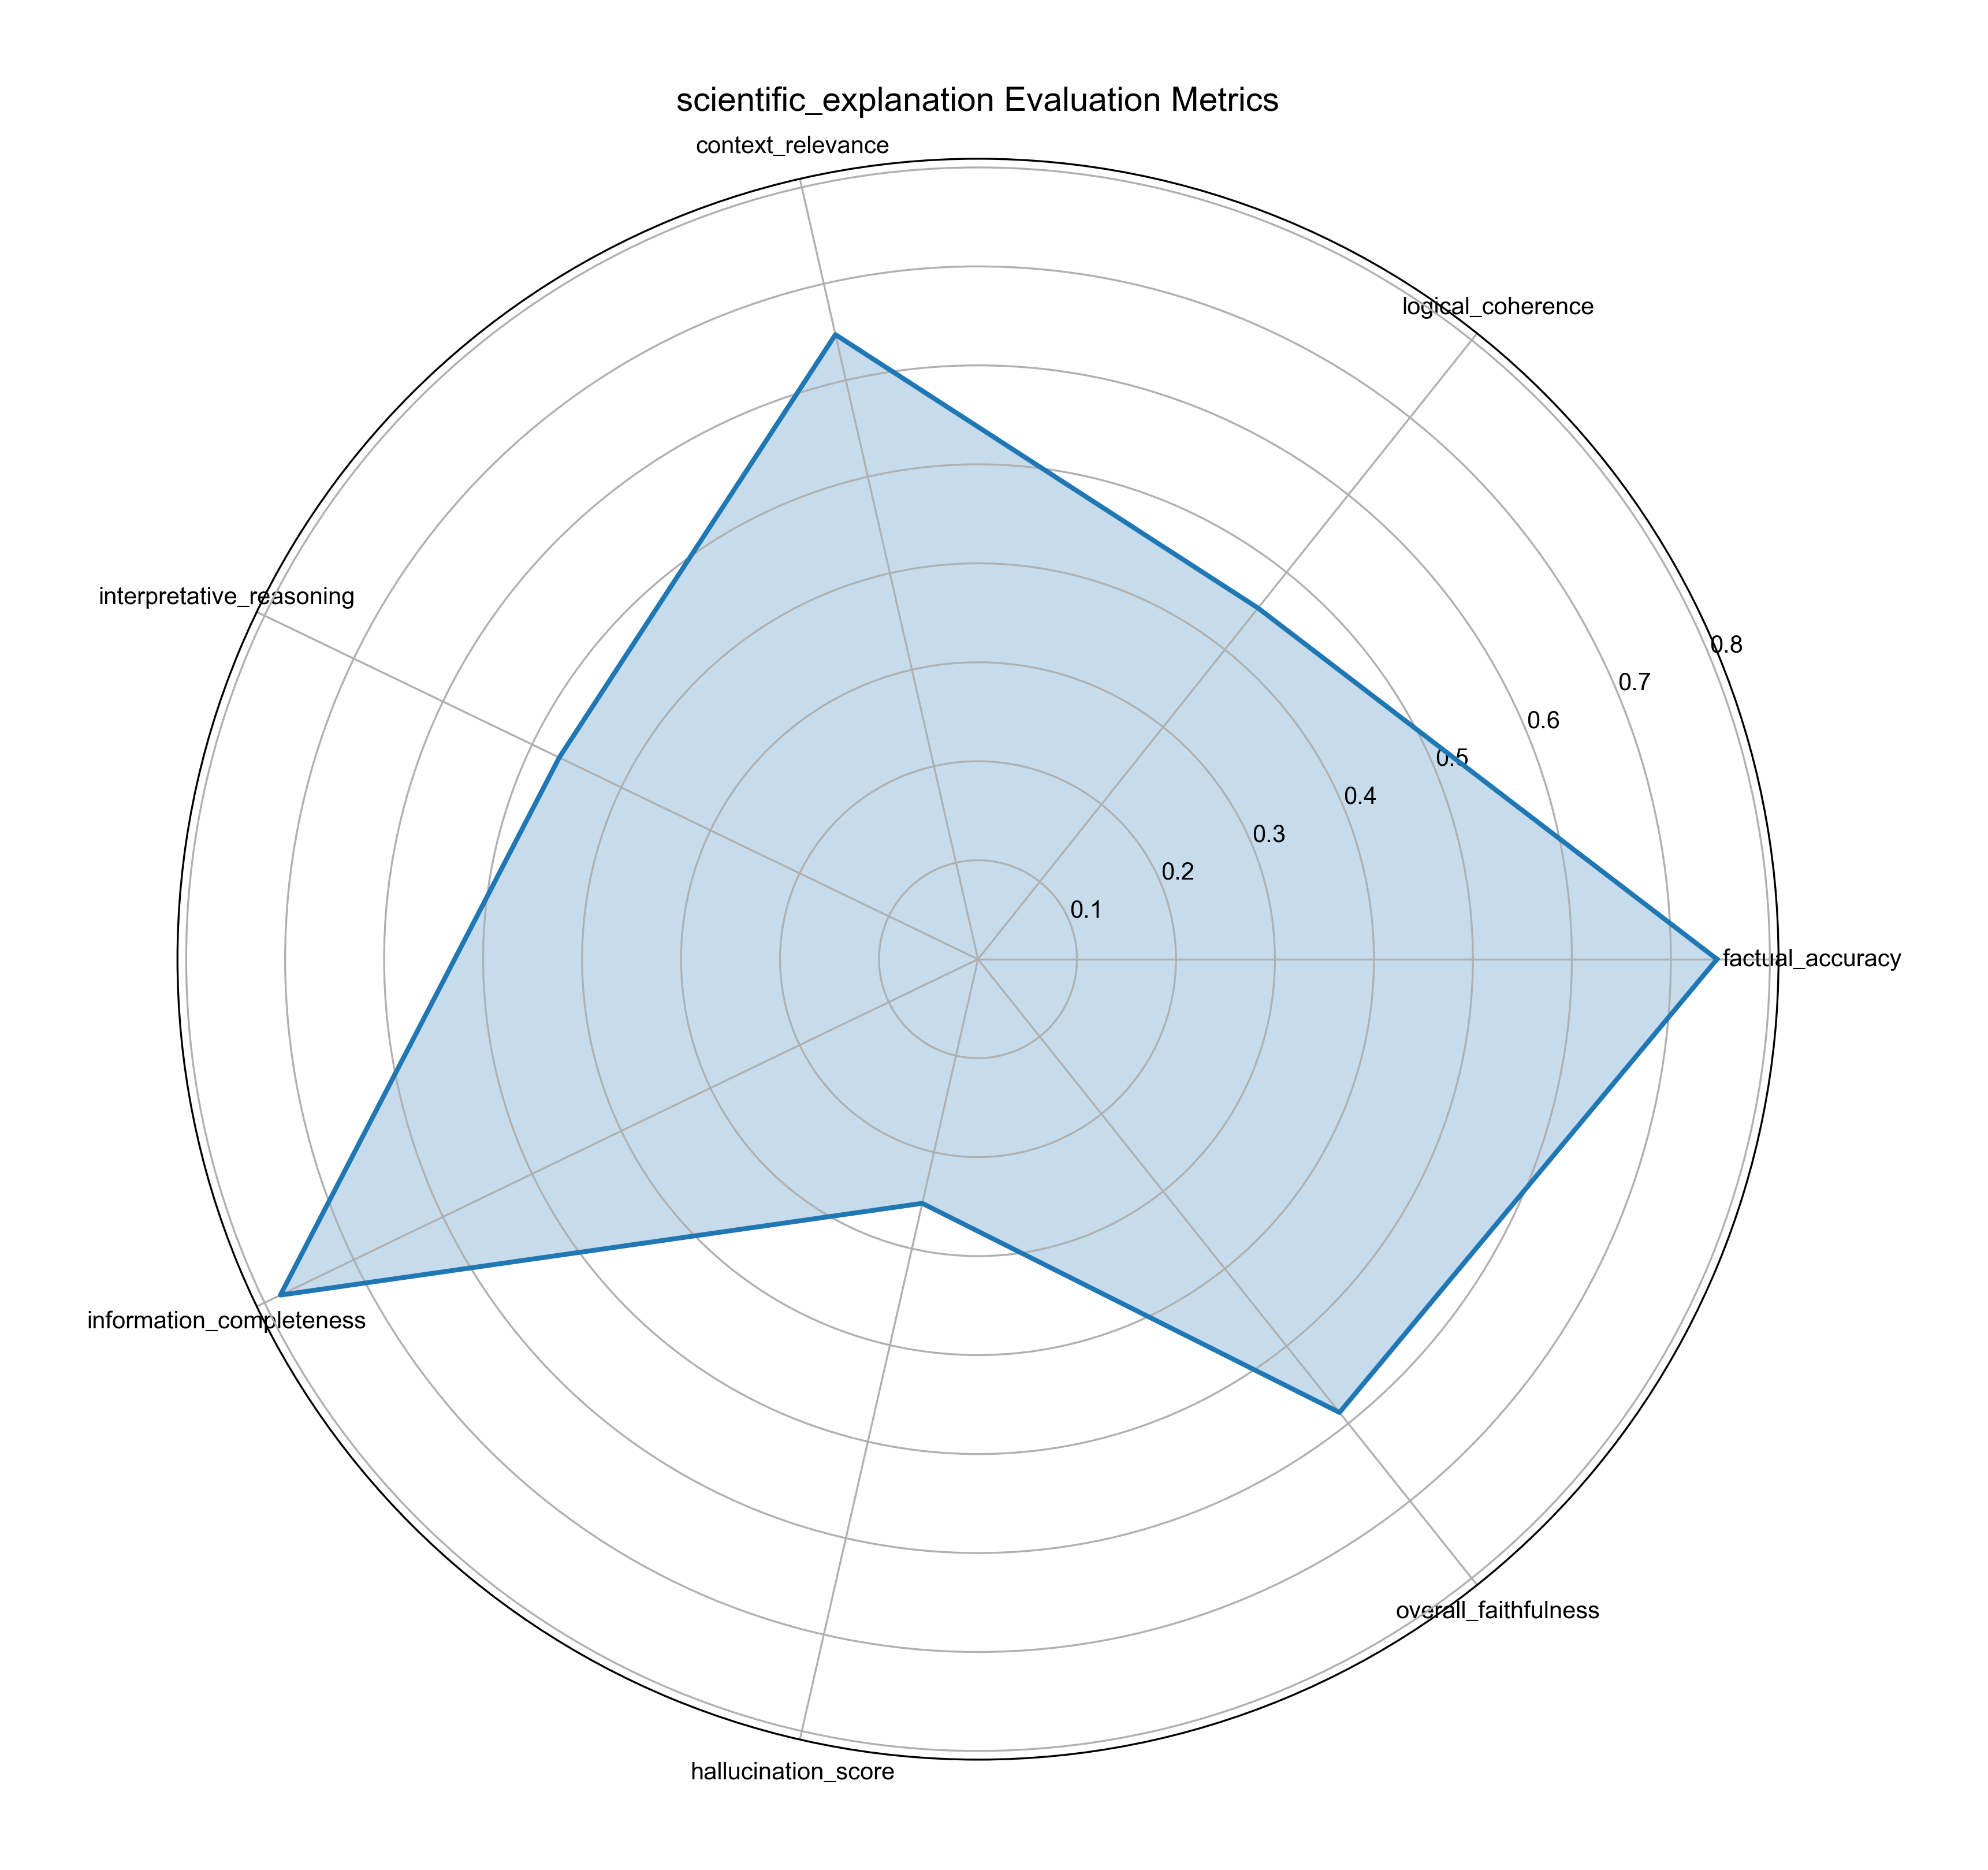
\includegraphics[width=0.6\textwidth]{figures/types/scientific_explanation_radar_gpt-4.png}
\caption{Scientific Explanation Performance Radar}
\label{fig:scientific_radar}
\end{figure}

\textbf{Analysis}:
\begin{itemize}
    \item GPT-3.5-Turbo demonstrates exceptional performance in scientific explanations, particularly in factual accuracy (0.8306) and information completeness (0.7858)
    \item Higher hallucination scores in this category suggest challenges in maintaining strict factual boundaries
    \item Logical coherence scores indicate room for improvement in structuring scientific arguments
\end{itemize}

\subsubsection{Technical Analysis}
For technical content, we evaluated the models' capability to handle detailed technical information and maintain accuracy in specialized contexts.

\begin{table}[!htbp]
\centering
\setlength{\tabcolsep}{4pt}  % Reduce table column spacing
\caption{Technical Analysis Metrics}
\label{tab:results_technical_metrics}
\begin{tabular}{|l|c|c|c|c|c|c|c|}
\hline
\textbf{Model} & \textbf{Fact.} & \textbf{Logic} & \textbf{Context} & \textbf{Interp.} 
& \textbf{Info.} & \textbf{Hall.} & \textbf{Overall} \\
\hline
GPT-3.5-Turbo & 0.8035 & 0.1930 & 0.6074 & 0.5386 & 0.6642 & 0.1938 & 0.5373 \\
GPT-4-Turbo & 0.7540 & 0.2071 & 0.5570 & 0.5874 & 0.7946 & 0.1653 & 0.5353 \\
GPT-4 & 0.8111 & 0.1670 & 0.7141 & 0.5911 & 0.6423 & 0.1571 & 0.5524 \\
\hline
\end{tabular}
\end{table}

\begin{figure}[!htbp]
\centering
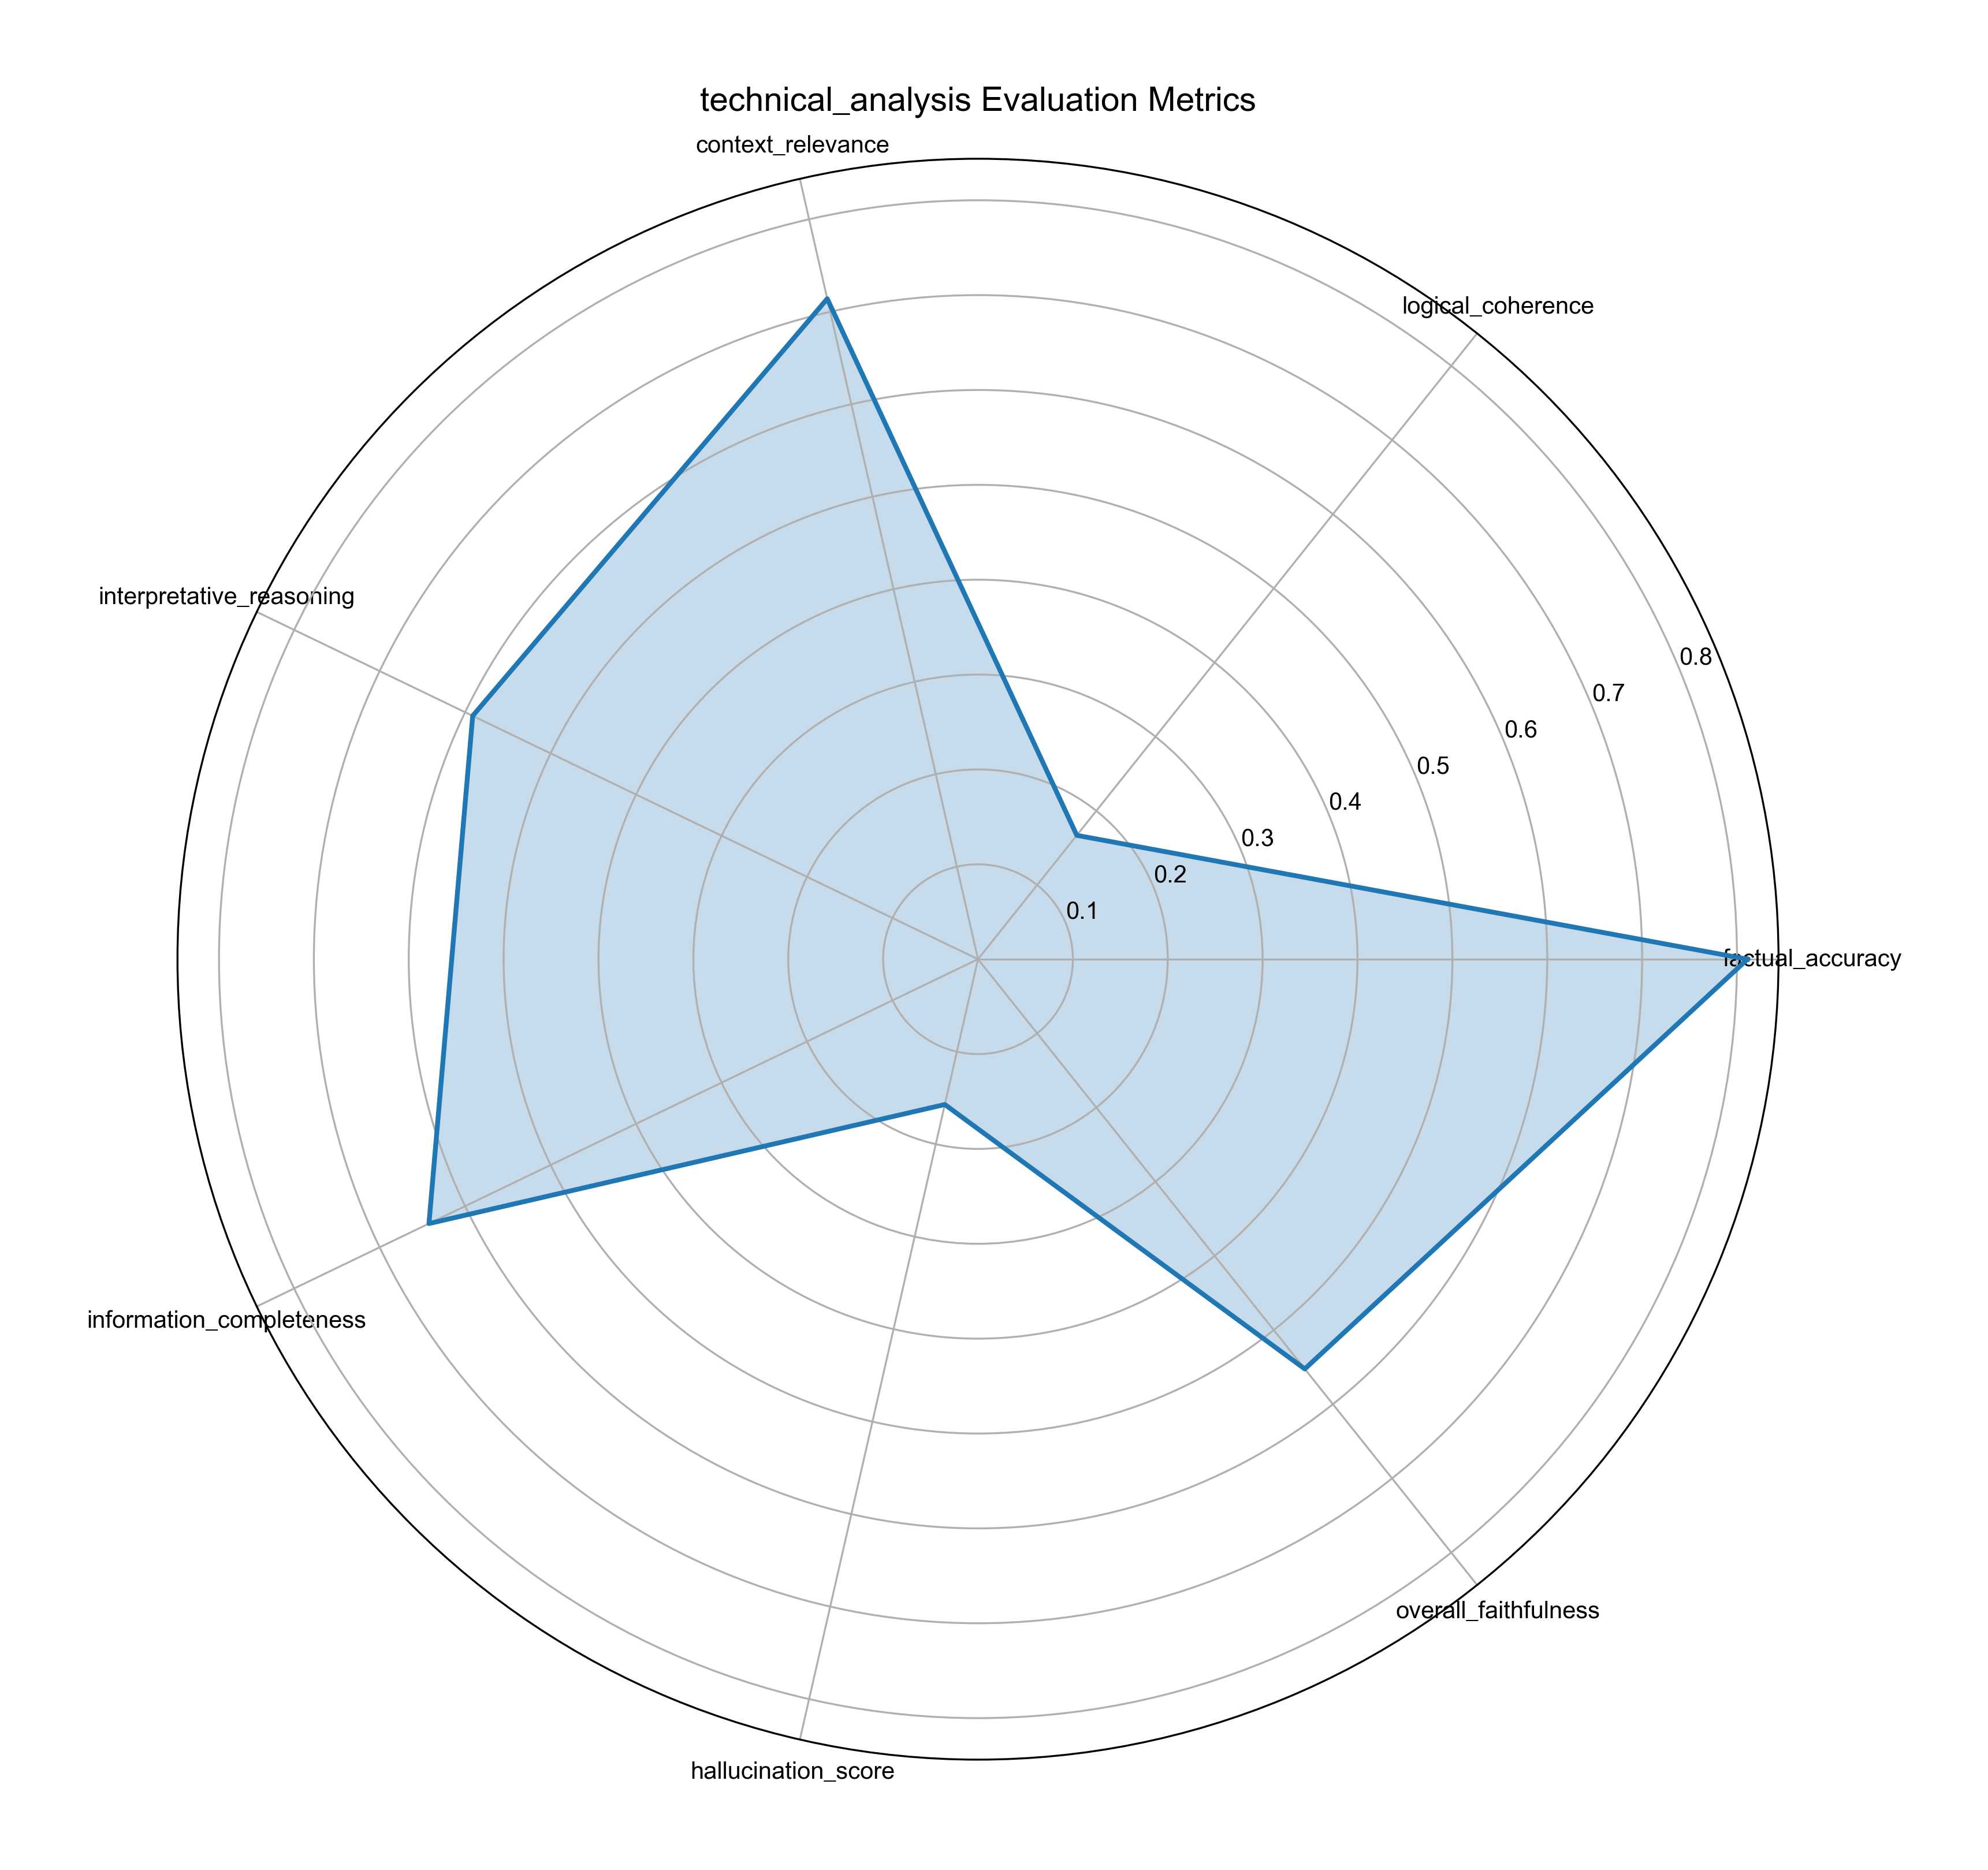
\includegraphics[width=0.6\textwidth]{figures/types/technical_analysis_radar_gpt-4.png}
\caption{Technical Analysis Performance Radar}
\label{fig:technical_radar}
\end{figure}

\textbf{Analysis}:
\begin{itemize}
    \item All models show improved performance in factual accuracy for technical content
    \item GPT-4 achieves the highest context relevance (0.7141), indicating better understanding of technical contexts
    \item Lower logical coherence scores suggest challenges in organizing technical information
\end{itemize}

\subsubsection{Medical Advice}
The medical advice evaluation assessed the models' ability to provide accurate and reliable health-related information.

\begin{table}[!htbp]
\centering
\setlength{\tabcolsep}{4pt}  % Reduce table column spacing
\caption{Medical Advice Metrics}
\label{tab:results_medical_metrics}
\begin{tabular}{|l|c|c|c|c|c|c|c|}
\hline
\textbf{Model} & \textbf{Fact.} & \textbf{Logic} & \textbf{Context} & \textbf{Interp.} 
& \textbf{Info.} & \textbf{Hall.} & \textbf{Overall} \\
\hline
GPT-3.5-Turbo & 0.9213 & 0.5800 & 0.6453 & 0.4023 & 0.7552 & 0.5496 & 0.6800 \\
GPT-4-Turbo & 0.7951 & 0.3453 & 0.6105 & 0.5156 & 0.8247 & 0.3218 & 0.6630 \\
GPT-4 & 0.9105 & 0.4630 & 0.6579 & 0.4605 & 0.7144 & 0.5809 & 0.6630 \\
\hline
\end{tabular}
\end{table}

\begin{figure}[!htbp]
\centering
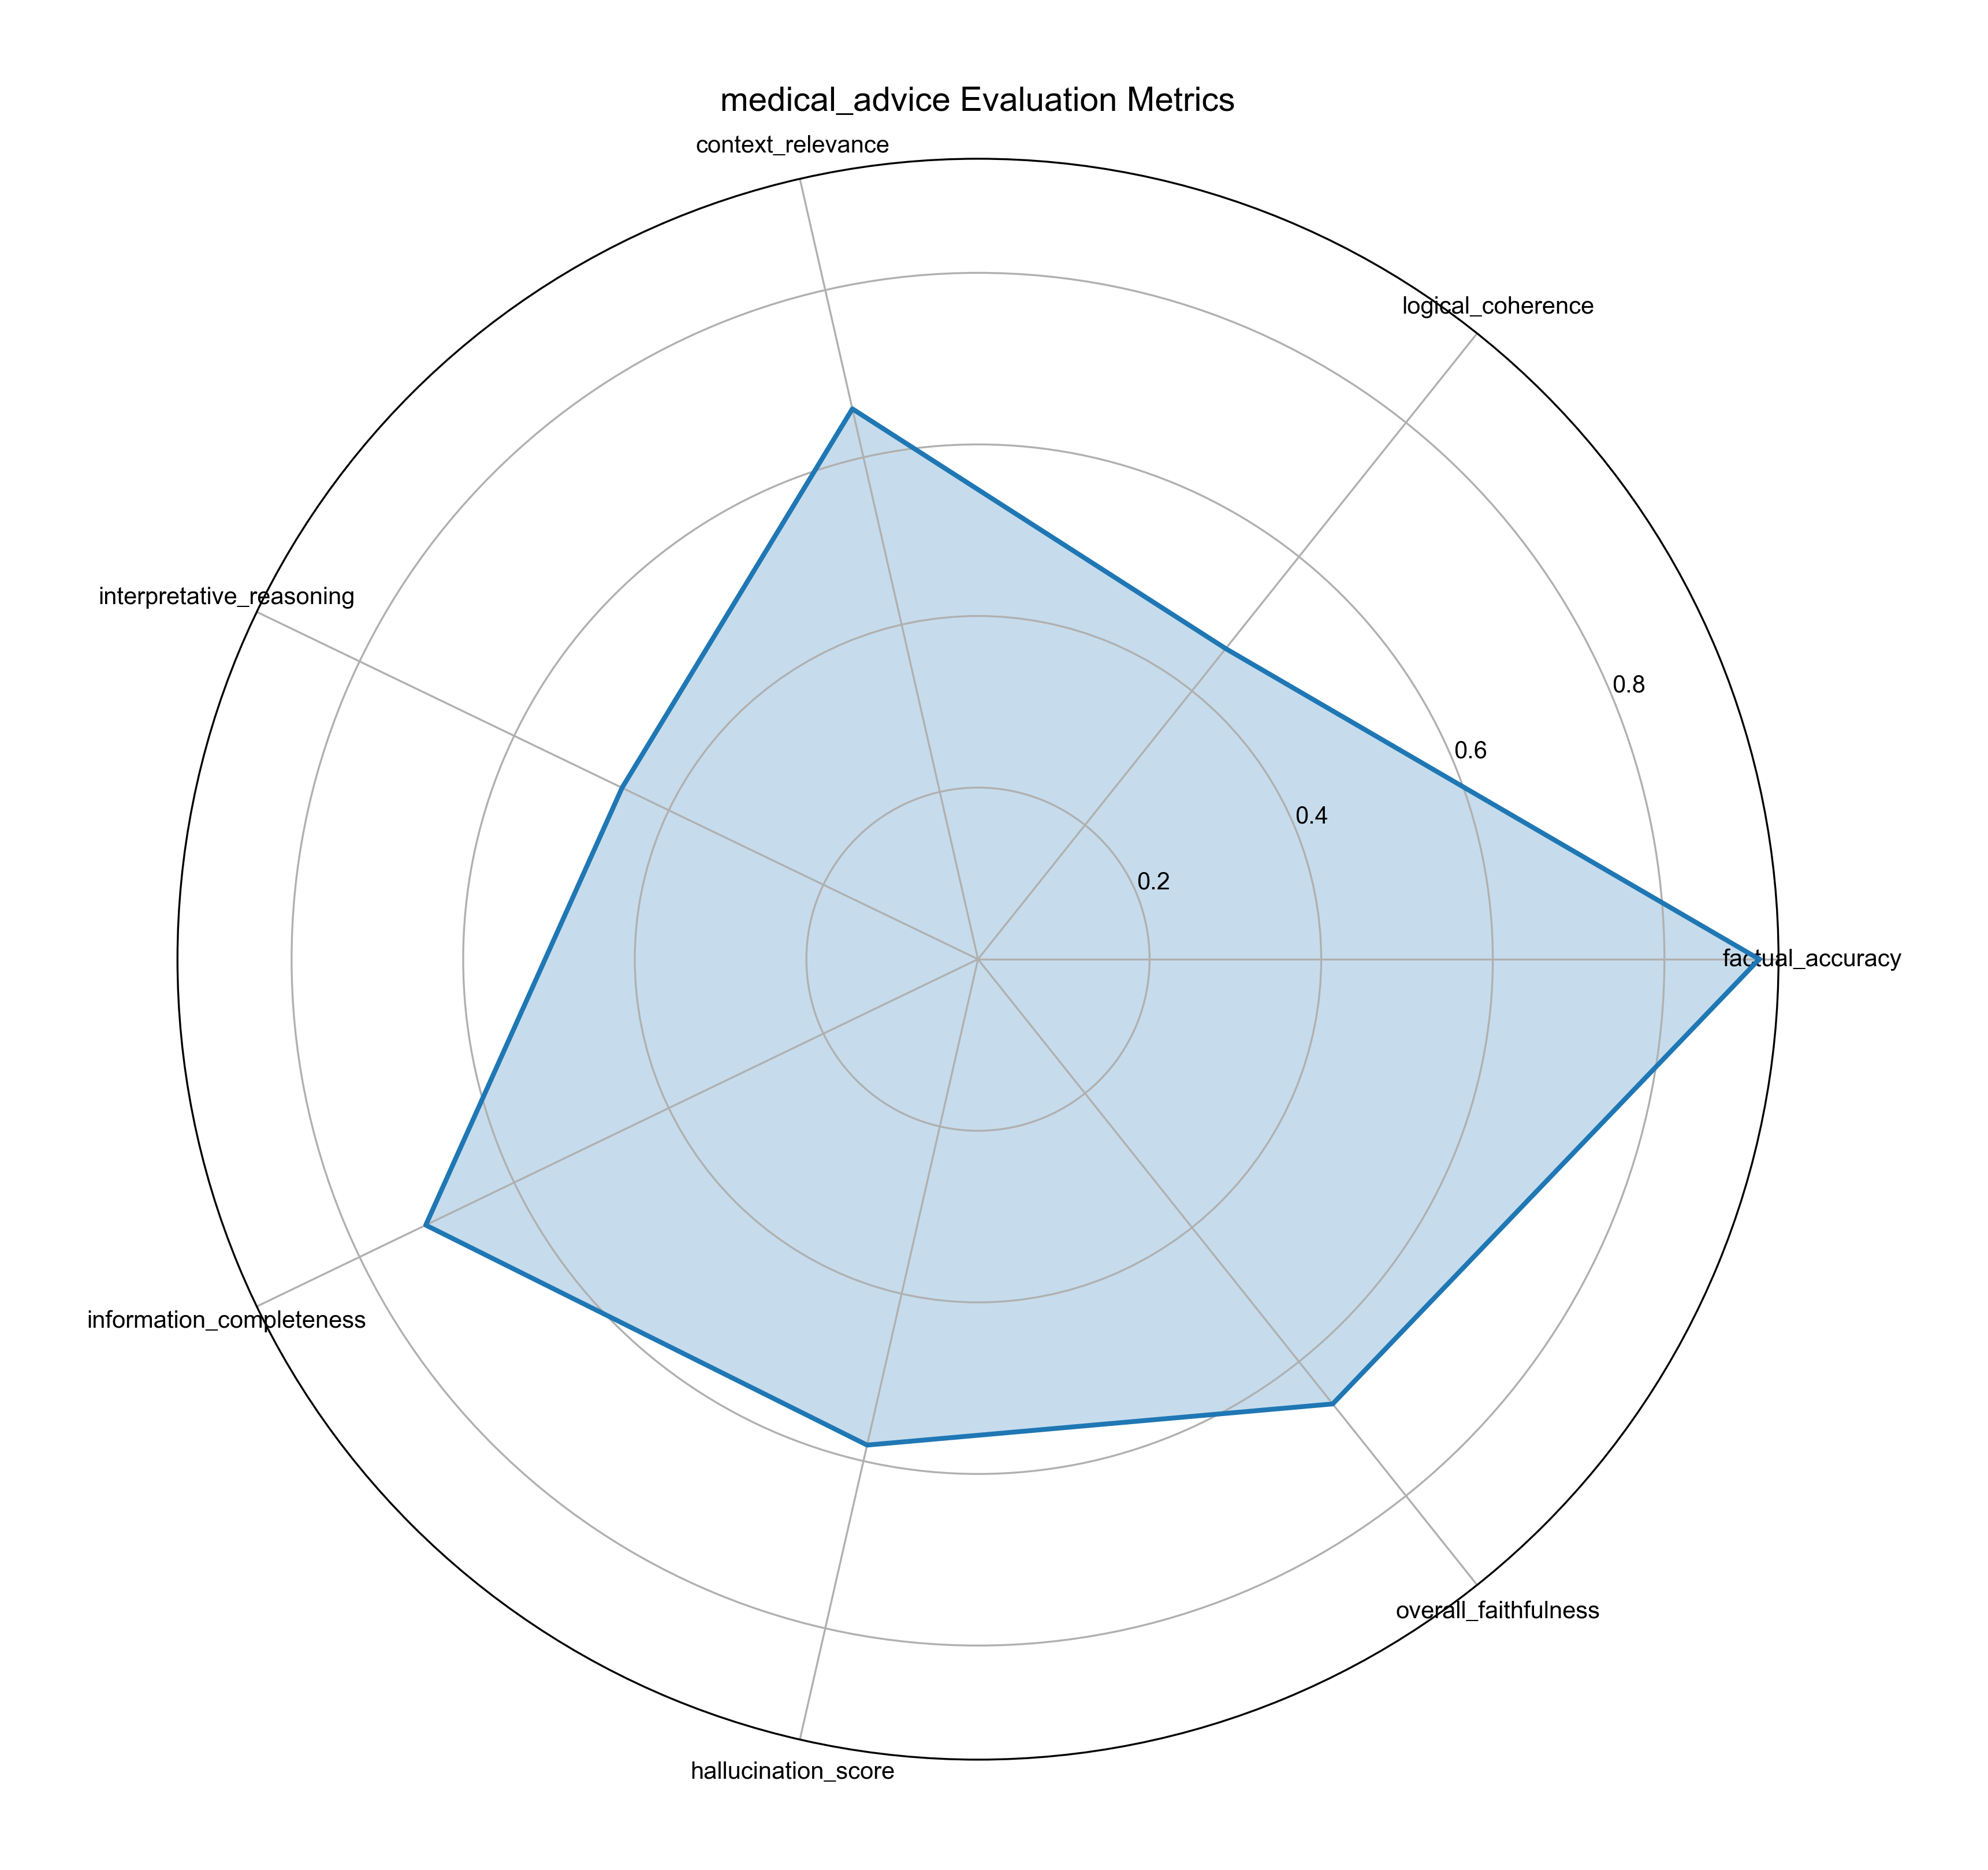
\includegraphics[width=0.6\textwidth]{figures/types/medical_advice_radar_gpt-4.png}
\caption{Medical Advice Performance Radar}
\label{fig:medical_radar}
\end{figure}

\textbf{Analysis}:
\begin{itemize}
    \item Notably high factual accuracy across all models, particularly in GPT-3.5-Turbo (0.9213)
    \item Strong information completeness scores reflect comprehensive medical responses
    \item Higher hallucination scores warrant attention in medical context
\end{itemize}

\subsubsection{Sample Type Comparison}
A comprehensive comparison across different sample types reveals how models adapt to varying content domains.

\begin{figure}[!htbp]
\centering
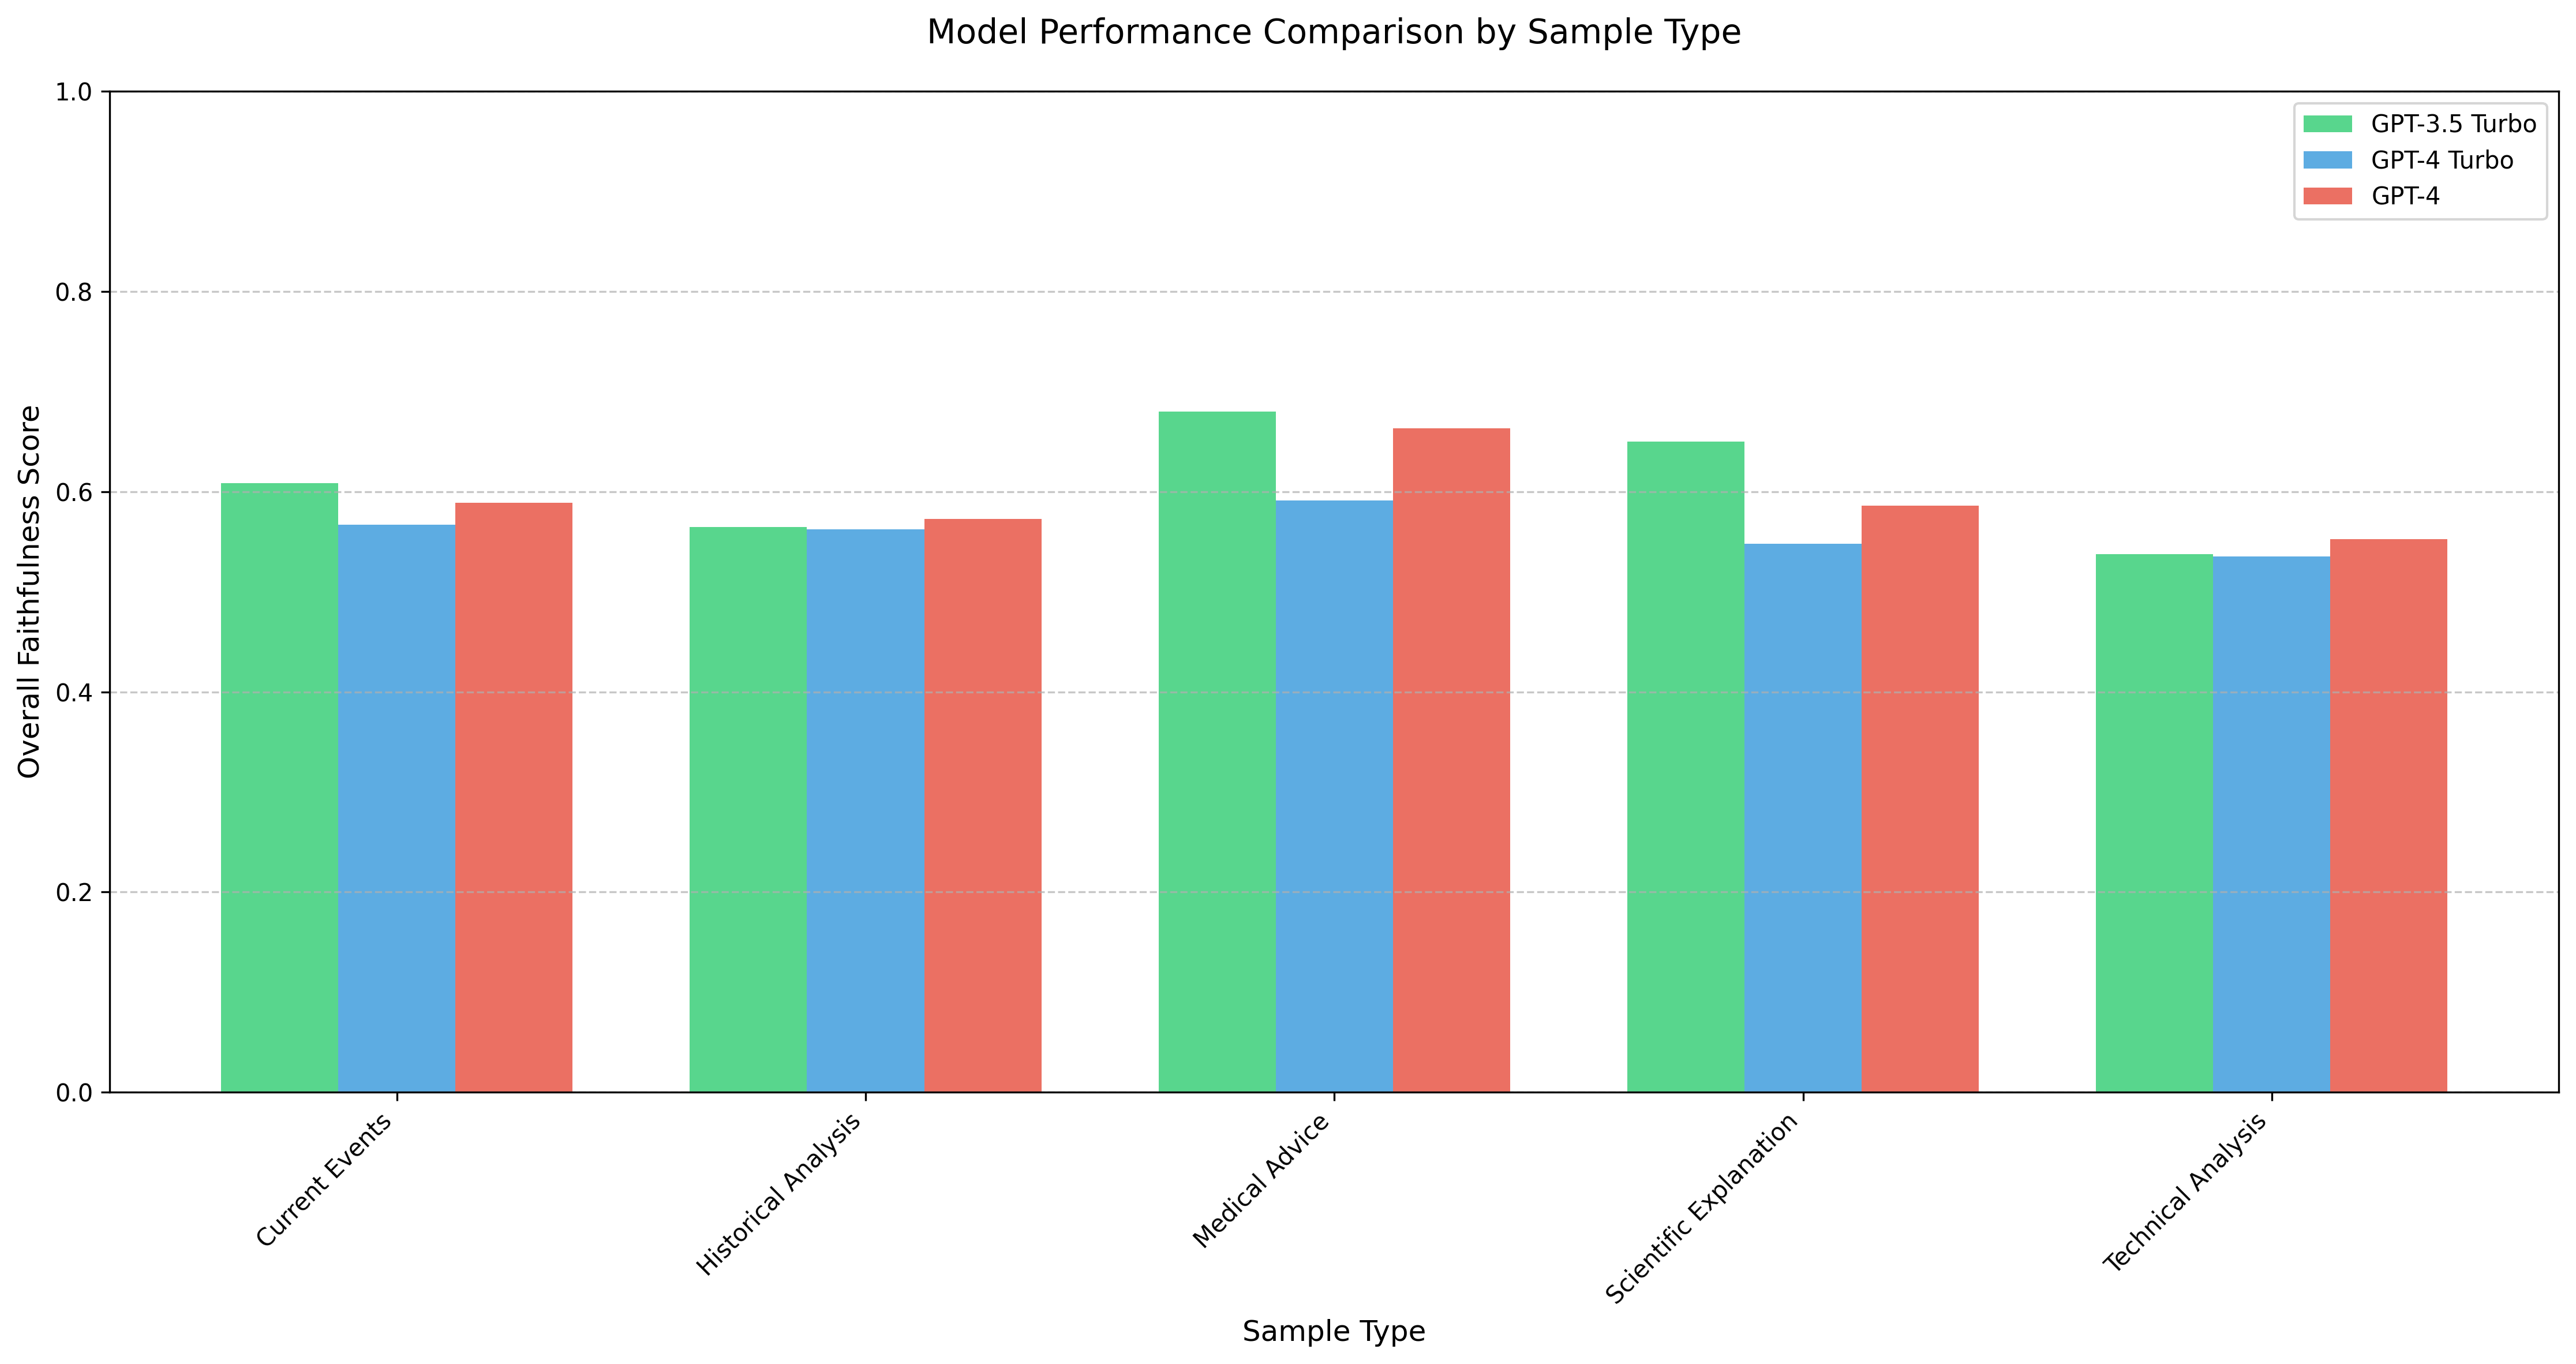
\includegraphics[width=0.8\textwidth]{figures/types/type_comparison.png}
\caption{Performance Comparison Across Sample Types}
\label{fig:type_comparison}
\end{figure}

\textbf{Cross-Type Analysis}:
\begin{itemize}
    \item Different content types present unique challenges for each model
    \item Performance patterns vary significantly across domains
    \item Some metrics show consistent trends regardless of content type
\end{itemize}

\subsection{Visualization Analysis}

\subsubsection{Metric Distribution Analysis}
The box plots provide insights into the statistical distribution and variability of each metric across models.

\begin{figure}[!htbp]
\centering
\begin{subfigure}[b]{0.32\textwidth}
    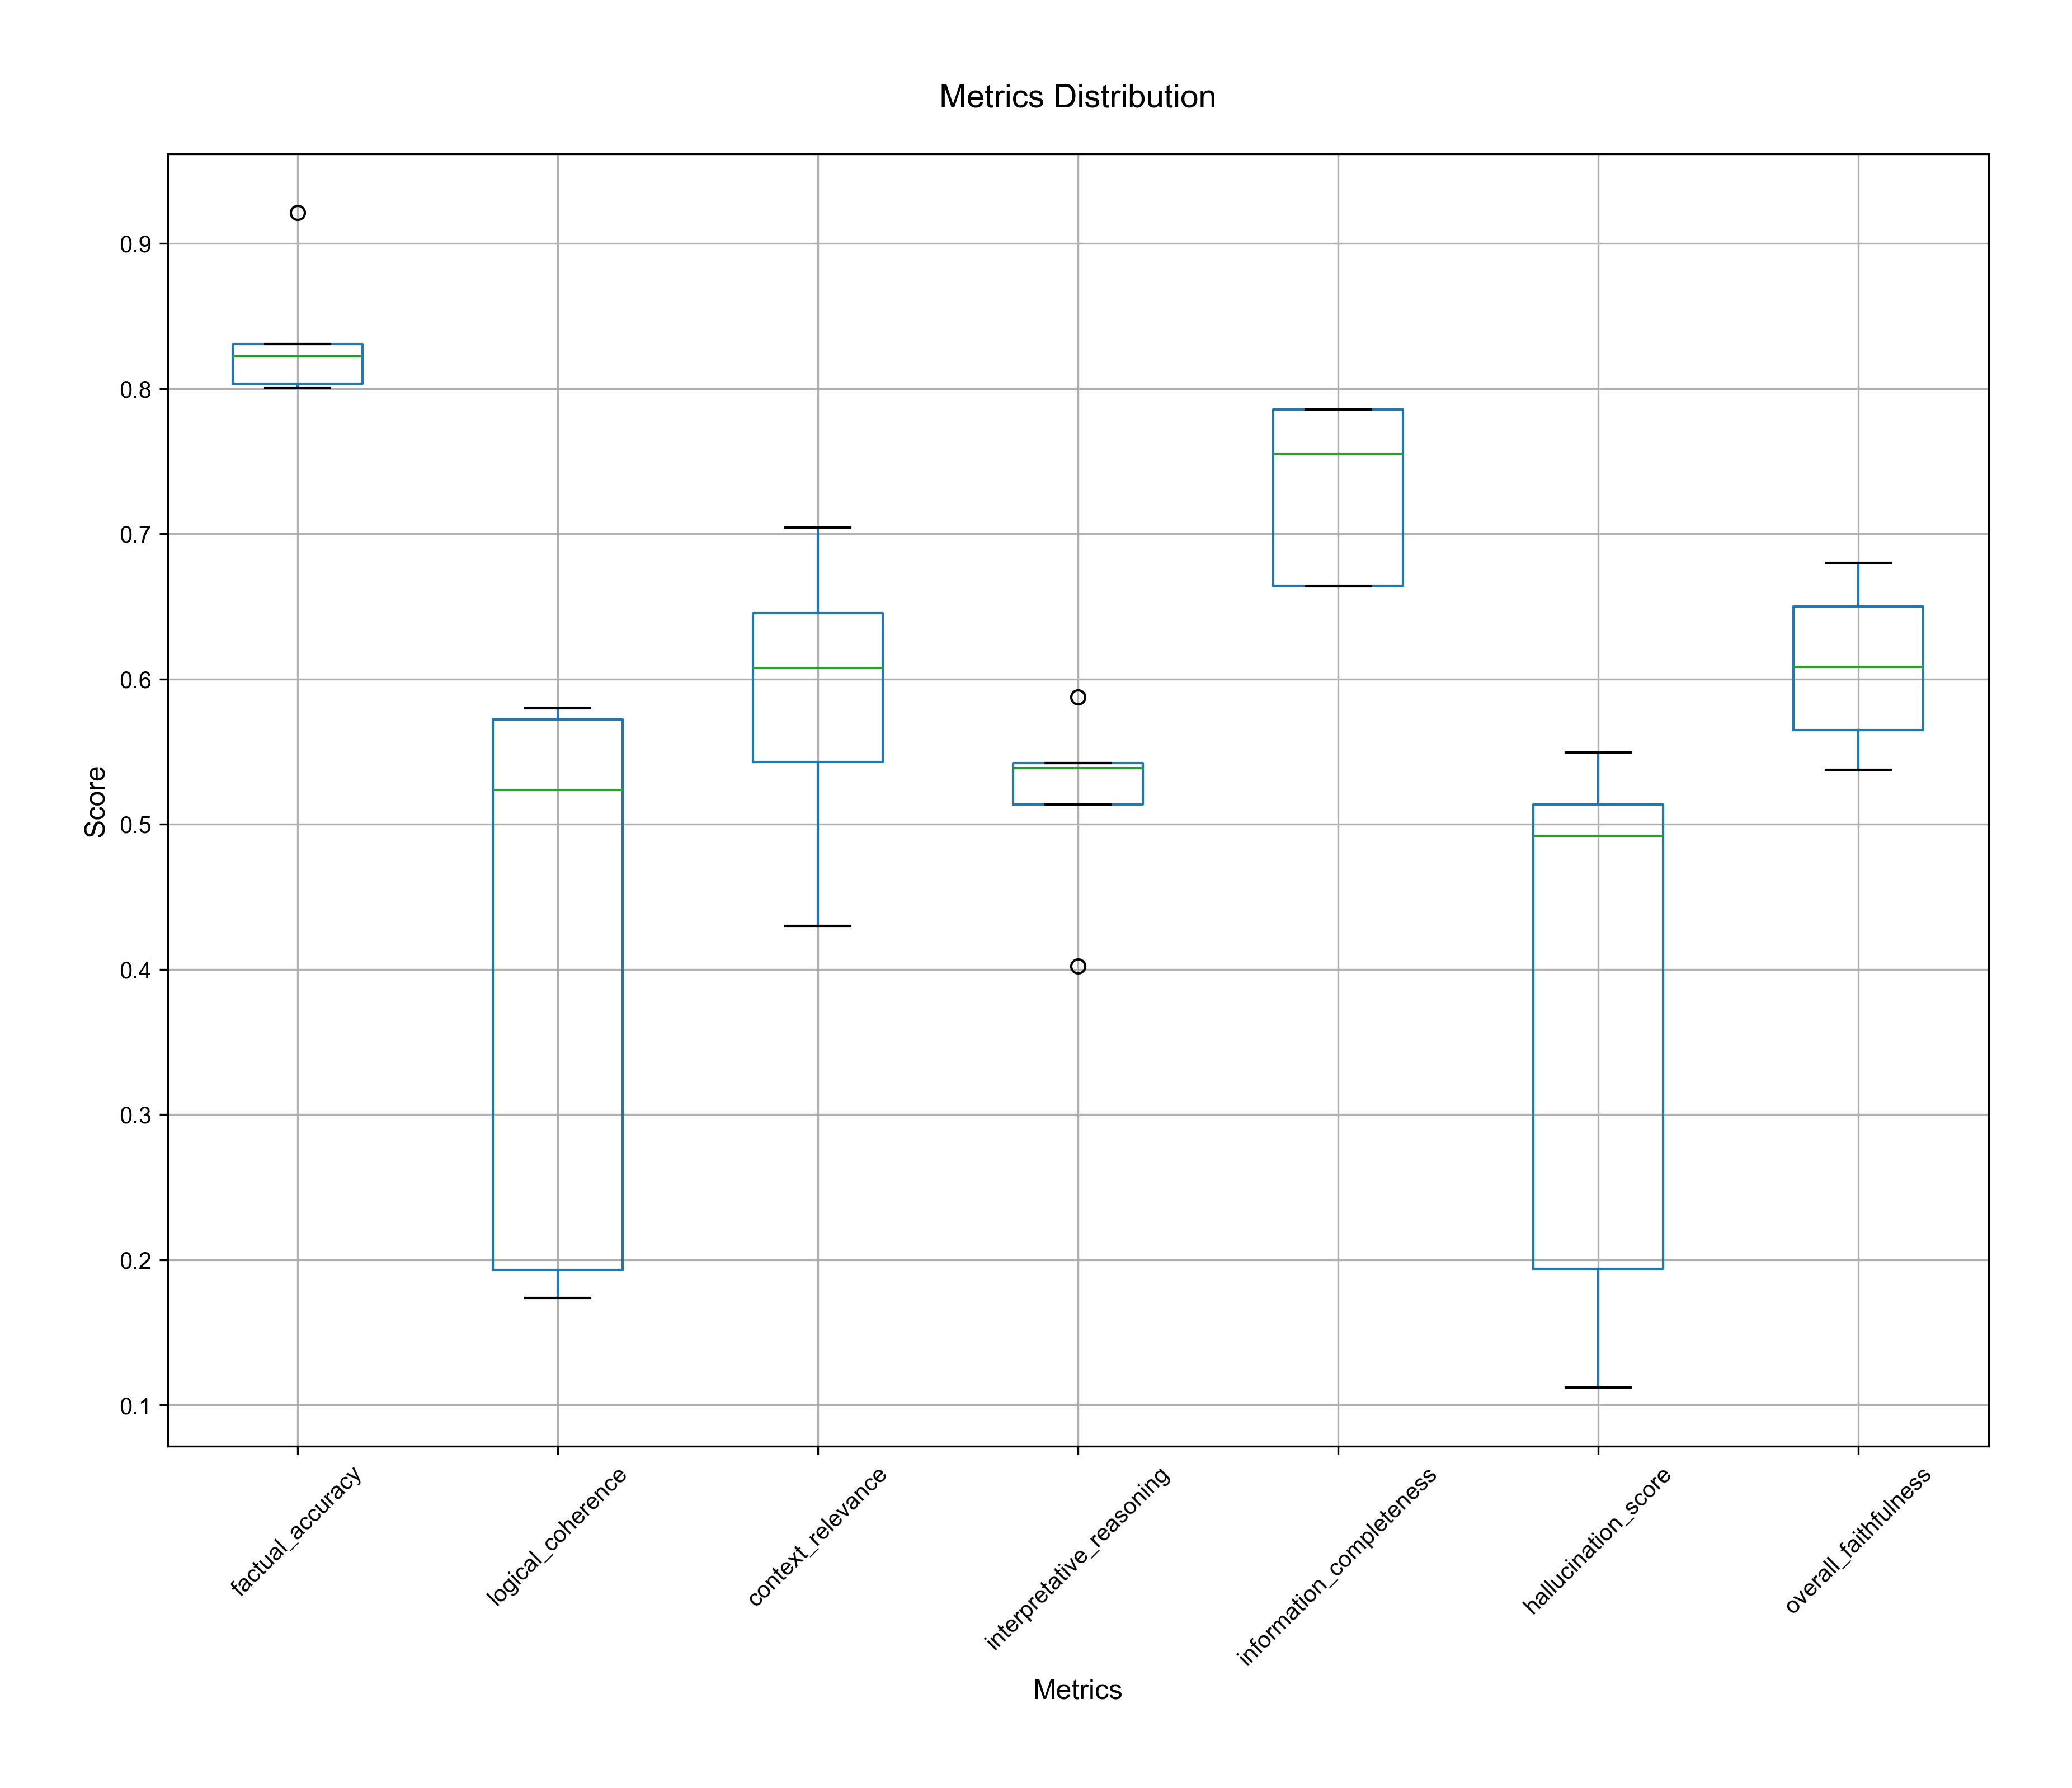
\includegraphics[width=\textwidth]{figures/visualization/metrics_boxplot_gpt-3.5-turbo.png}
    \caption{GPT-3.5-Turbo}
    \label{fig:metrics_boxplot_gpt35}
\end{subfigure}
\hfill
\begin{subfigure}[b]{0.32\textwidth}
    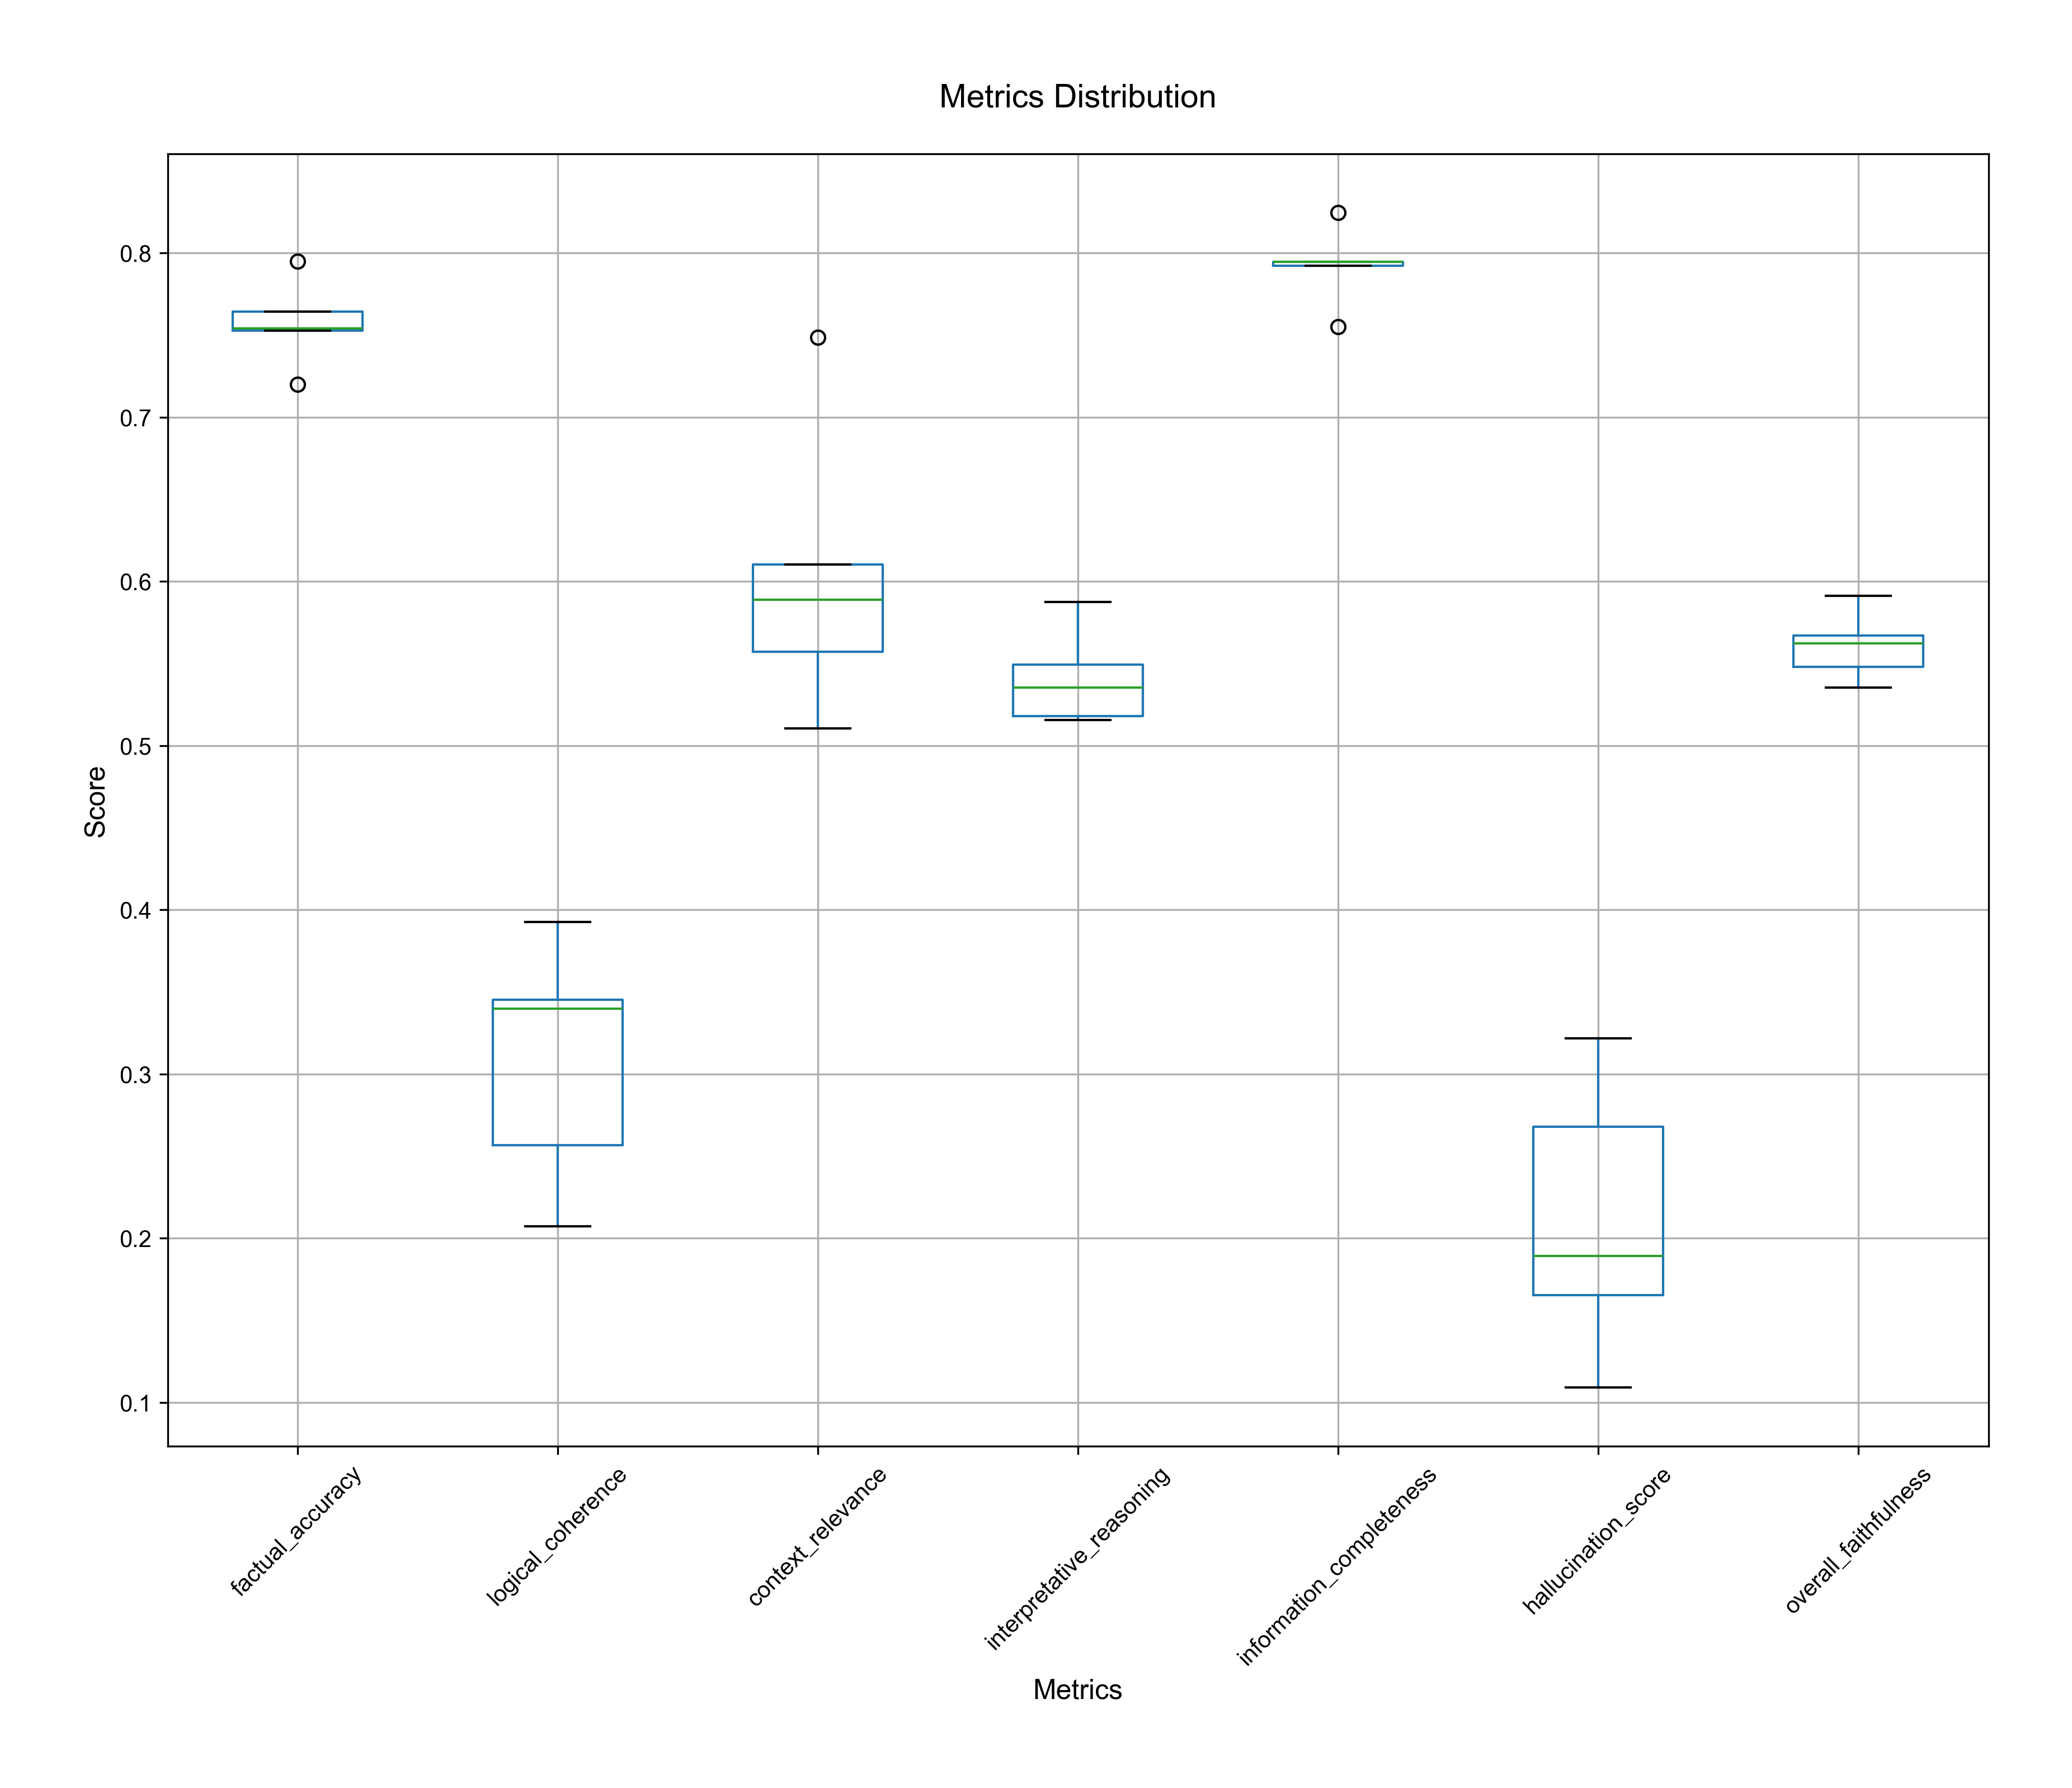
\includegraphics[width=\textwidth]{figures/visualization/metrics_boxplot_gpt-4-turbo.png}
    \caption{GPT-4-Turbo}
    \label{fig:metrics_boxplot_gpt4t}
\end{subfigure}
\hfill
\begin{subfigure}[b]{0.32\textwidth}
    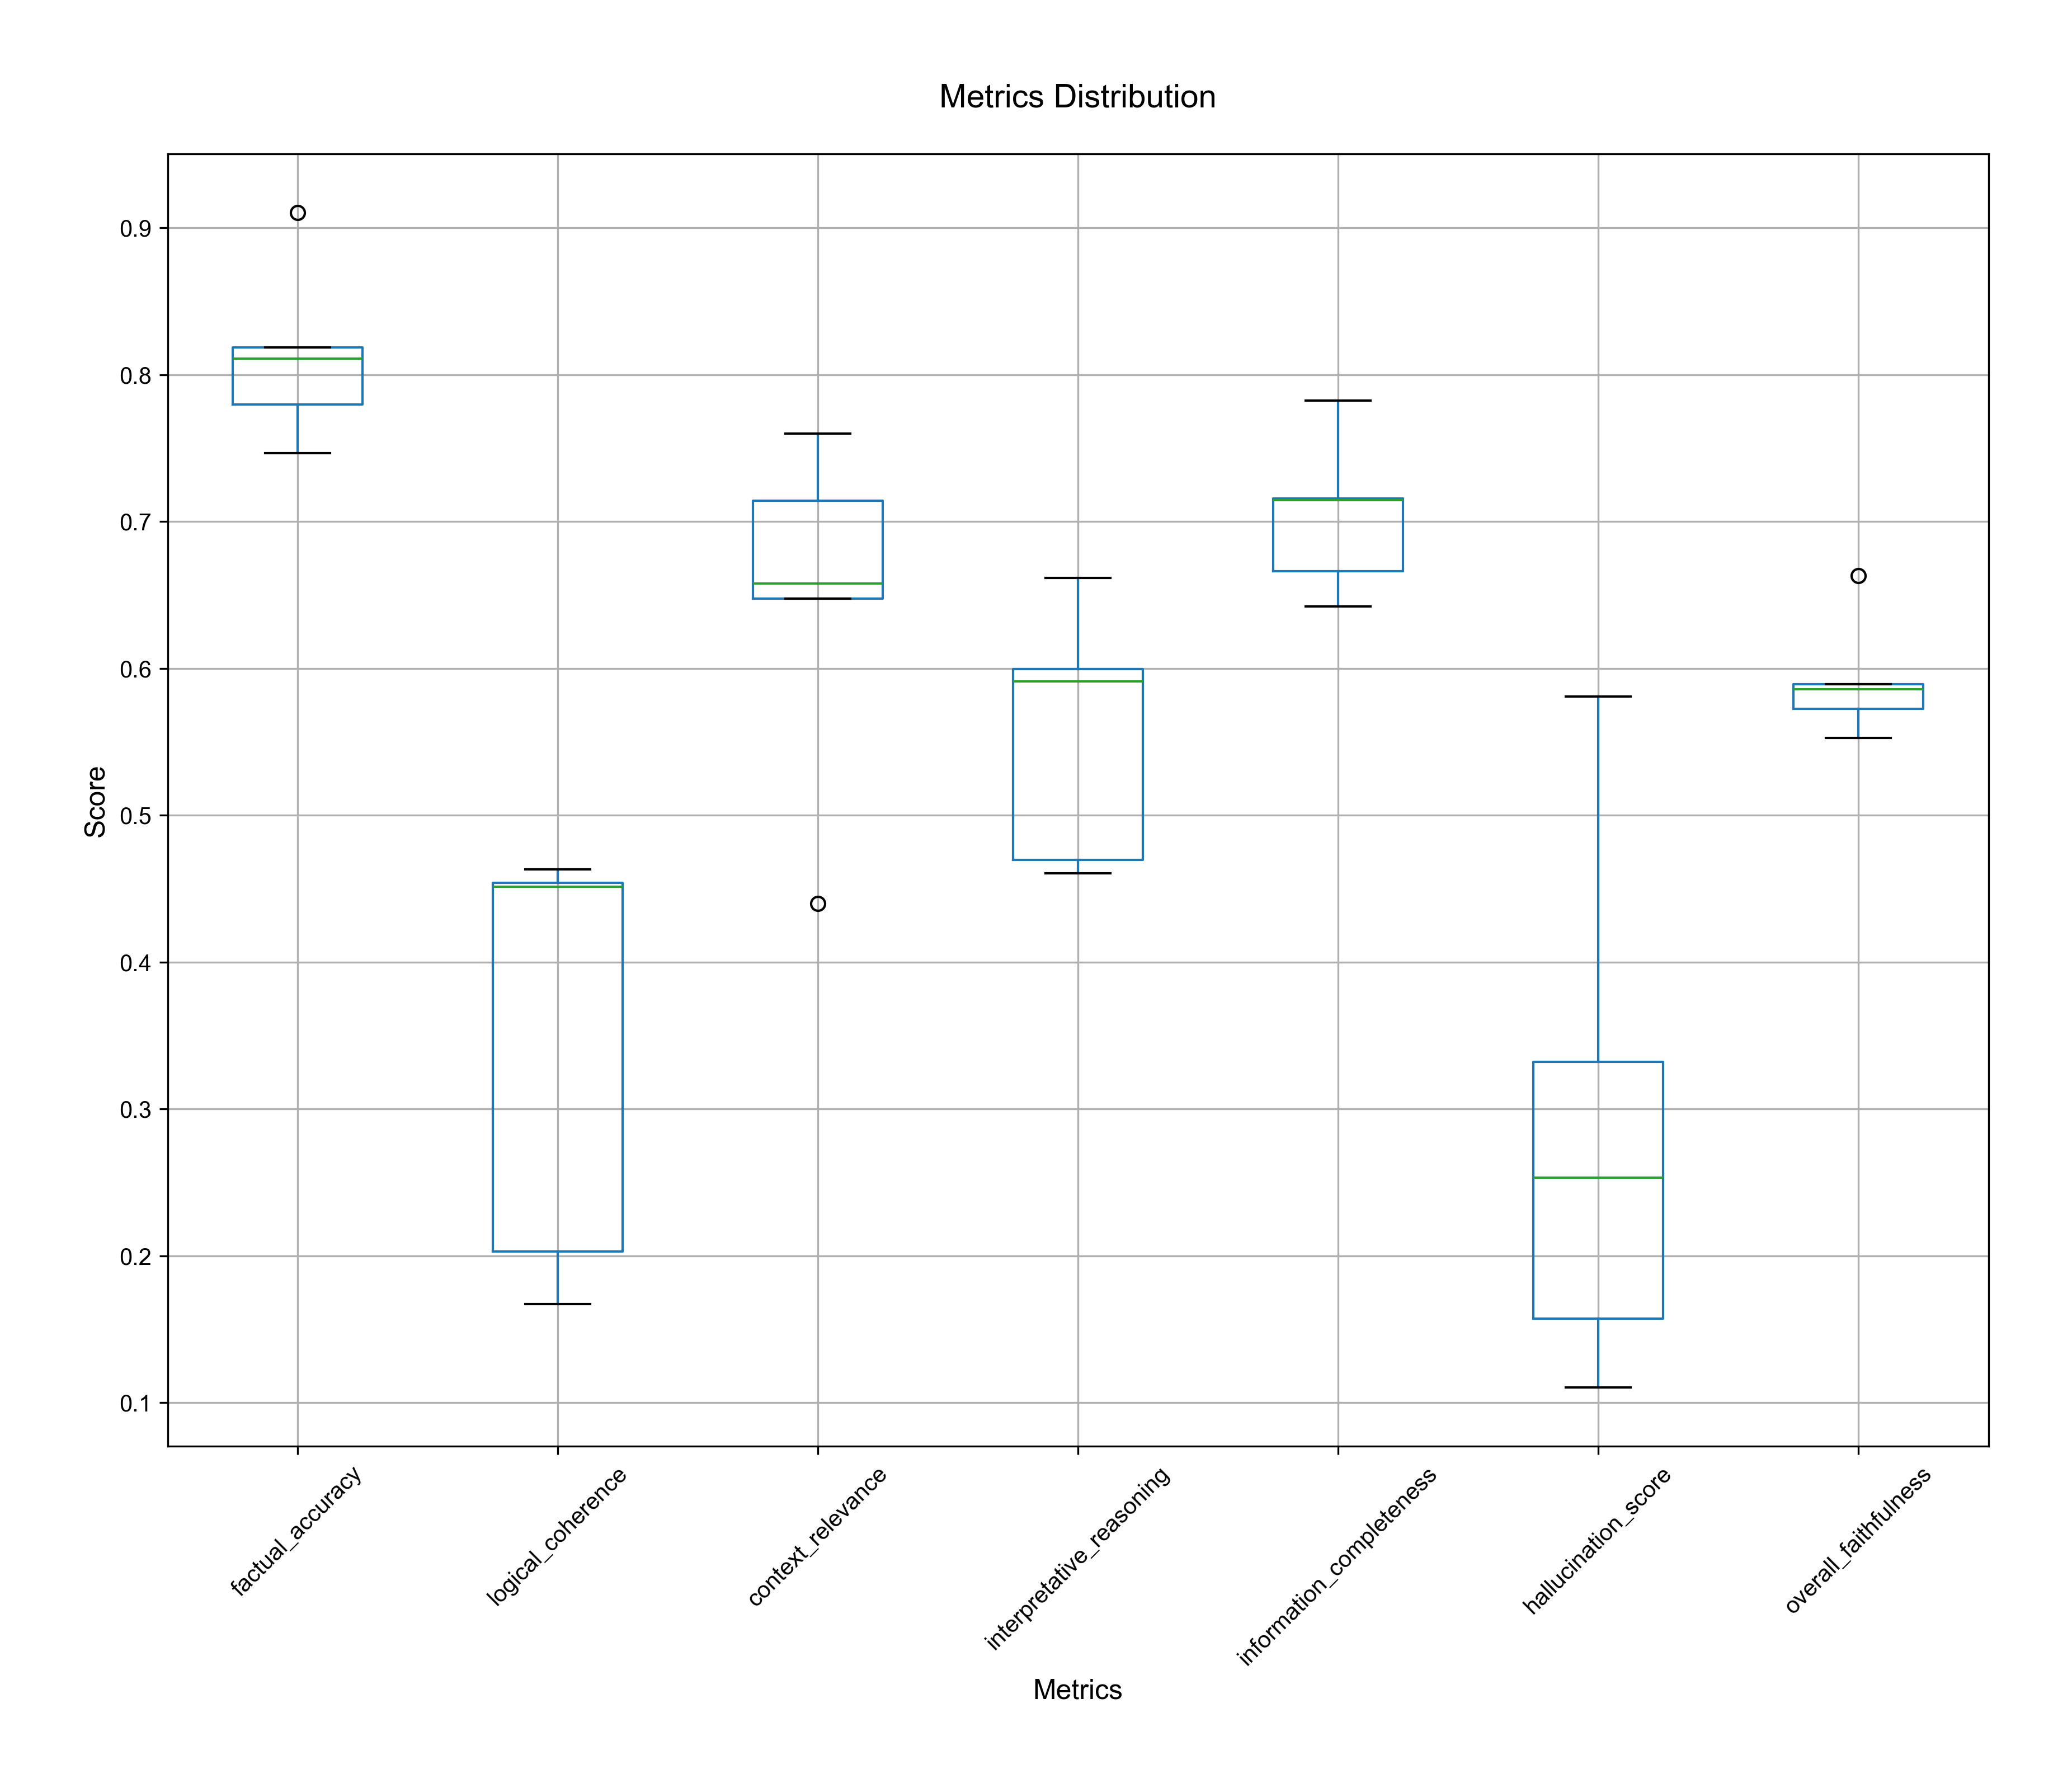
\includegraphics[width=\textwidth]{figures/visualization/metrics_boxplot_gpt-4.png}
    \caption{GPT-4}
    \label{fig:metrics_boxplot_gpt4}
\end{subfigure}
\caption{Metric Score Distributions by Model}
\label{fig:metrics_boxplots}
\end{figure}

\textbf{Distribution Insights}:
\begin{itemize}
    \item Factual accuracy shows the most consistent distribution across models
    \item Logical coherence exhibits the widest range of scores
    \item Hallucination scores show significant outliers, particularly in GPT-3.5-Turbo
\end{itemize}

\subsubsection{Correlation Analysis}
Heat maps visualize the relationships between different metrics, revealing important patterns and dependencies.

\begin{figure}[!htbp]
\centering
\begin{subfigure}[b]{0.32\textwidth}
    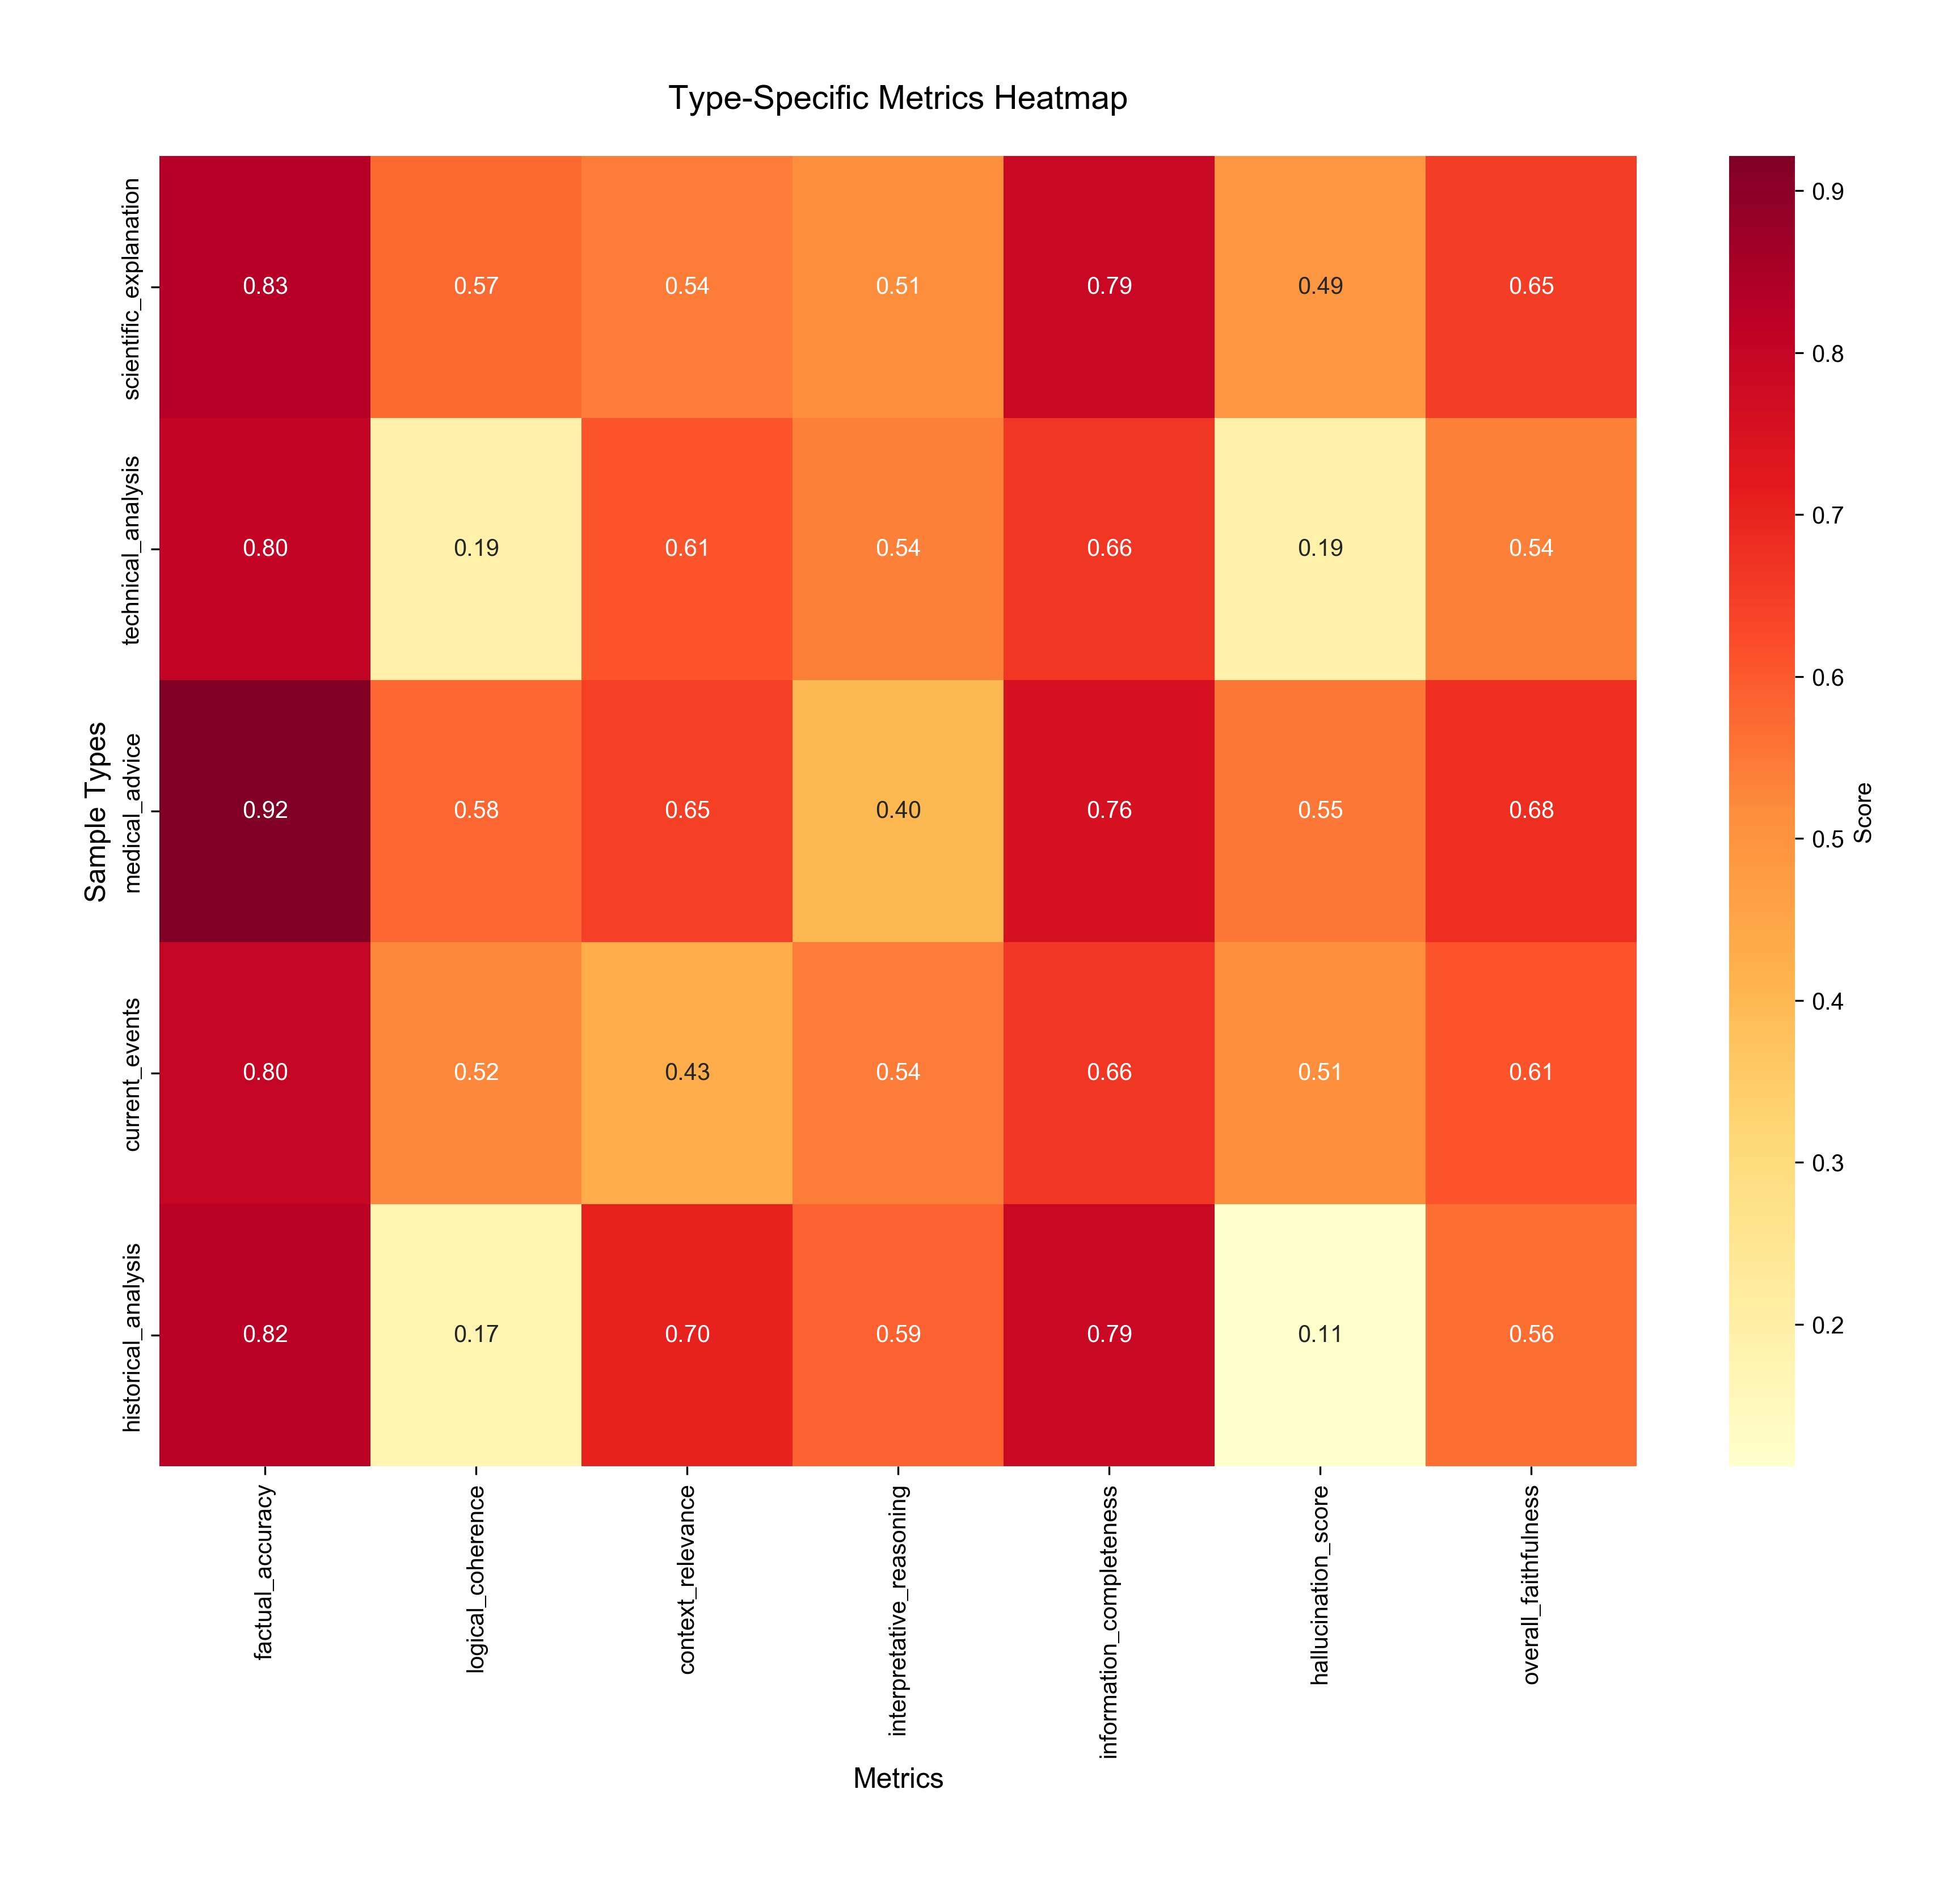
\includegraphics[width=\textwidth]{figures/visualization/metrics_heatmap_gpt-3.5-turbo.png}
    \caption{GPT-3.5-Turbo}
    \label{fig:metrics_heatmap_gpt35}
\end{subfigure}
\hfill
\begin{subfigure}[b]{0.32\textwidth}
    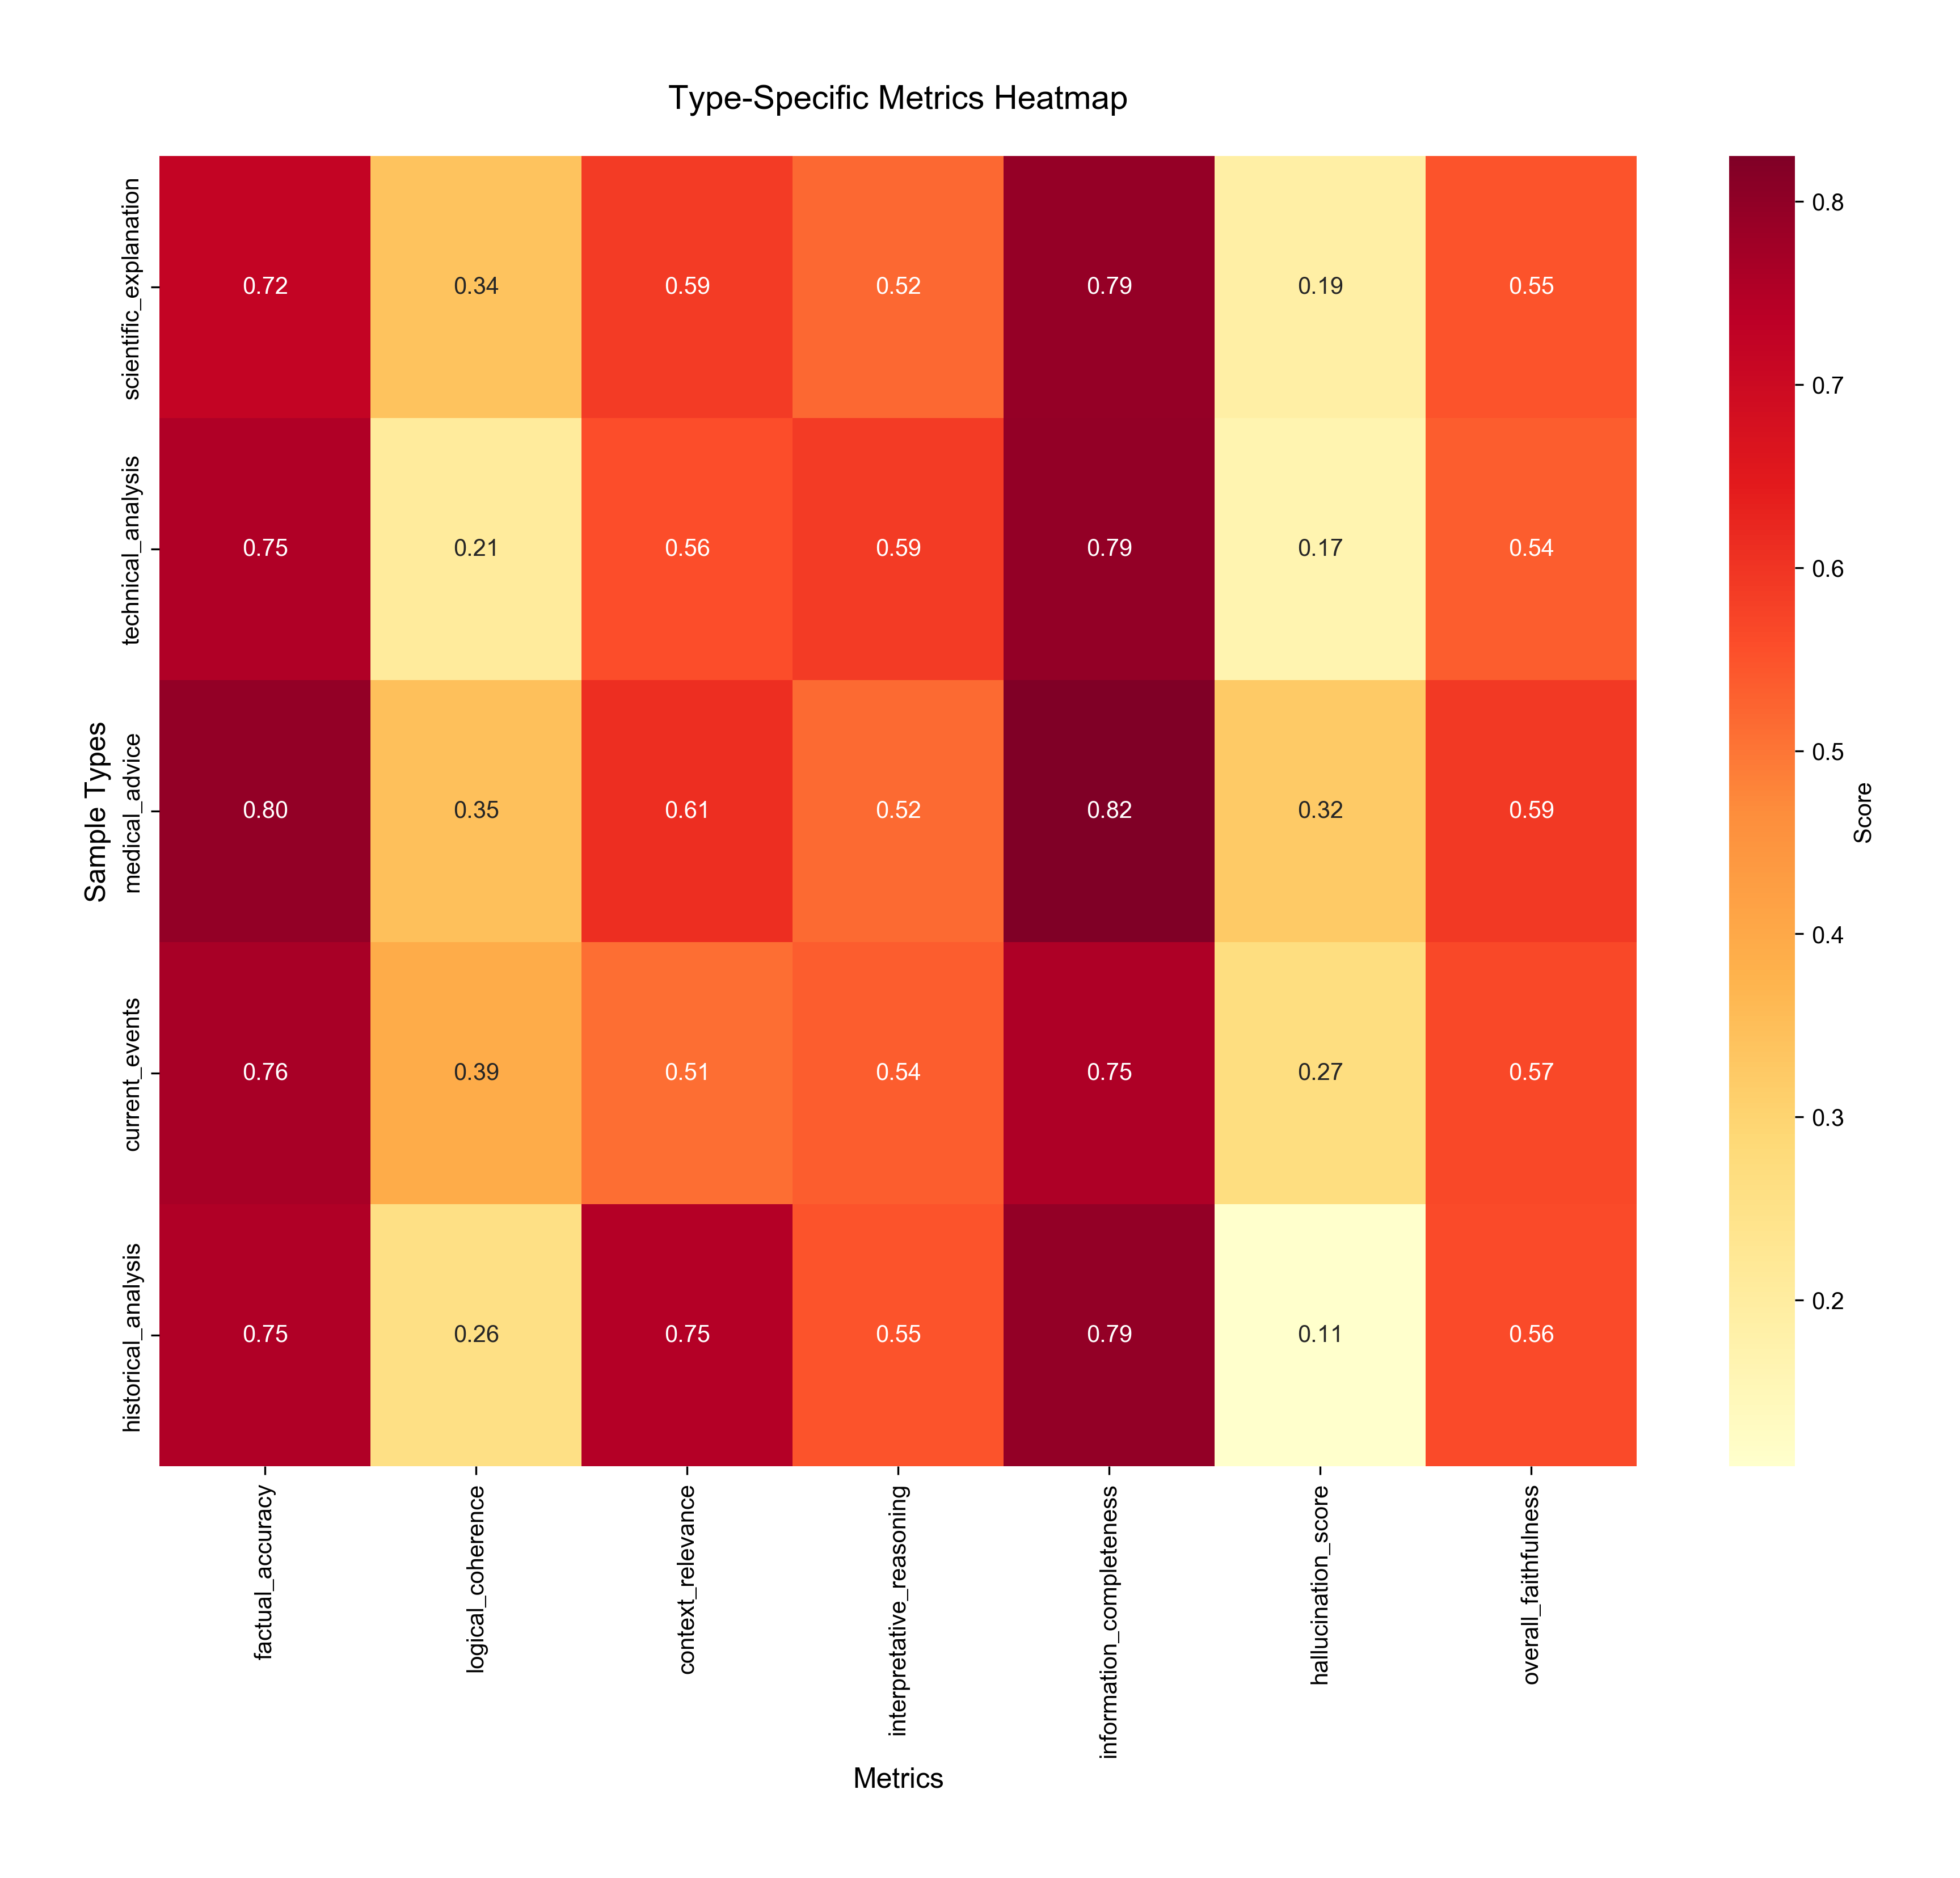
\includegraphics[width=\textwidth]{figures/visualization/metrics_heatmap_gpt-4-turbo.png}
    \caption{GPT-4-Turbo}
    \label{fig:metrics_heatmap_gpt4t}
\end{subfigure}
\hfill
\begin{subfigure}[b]{0.32\textwidth}
    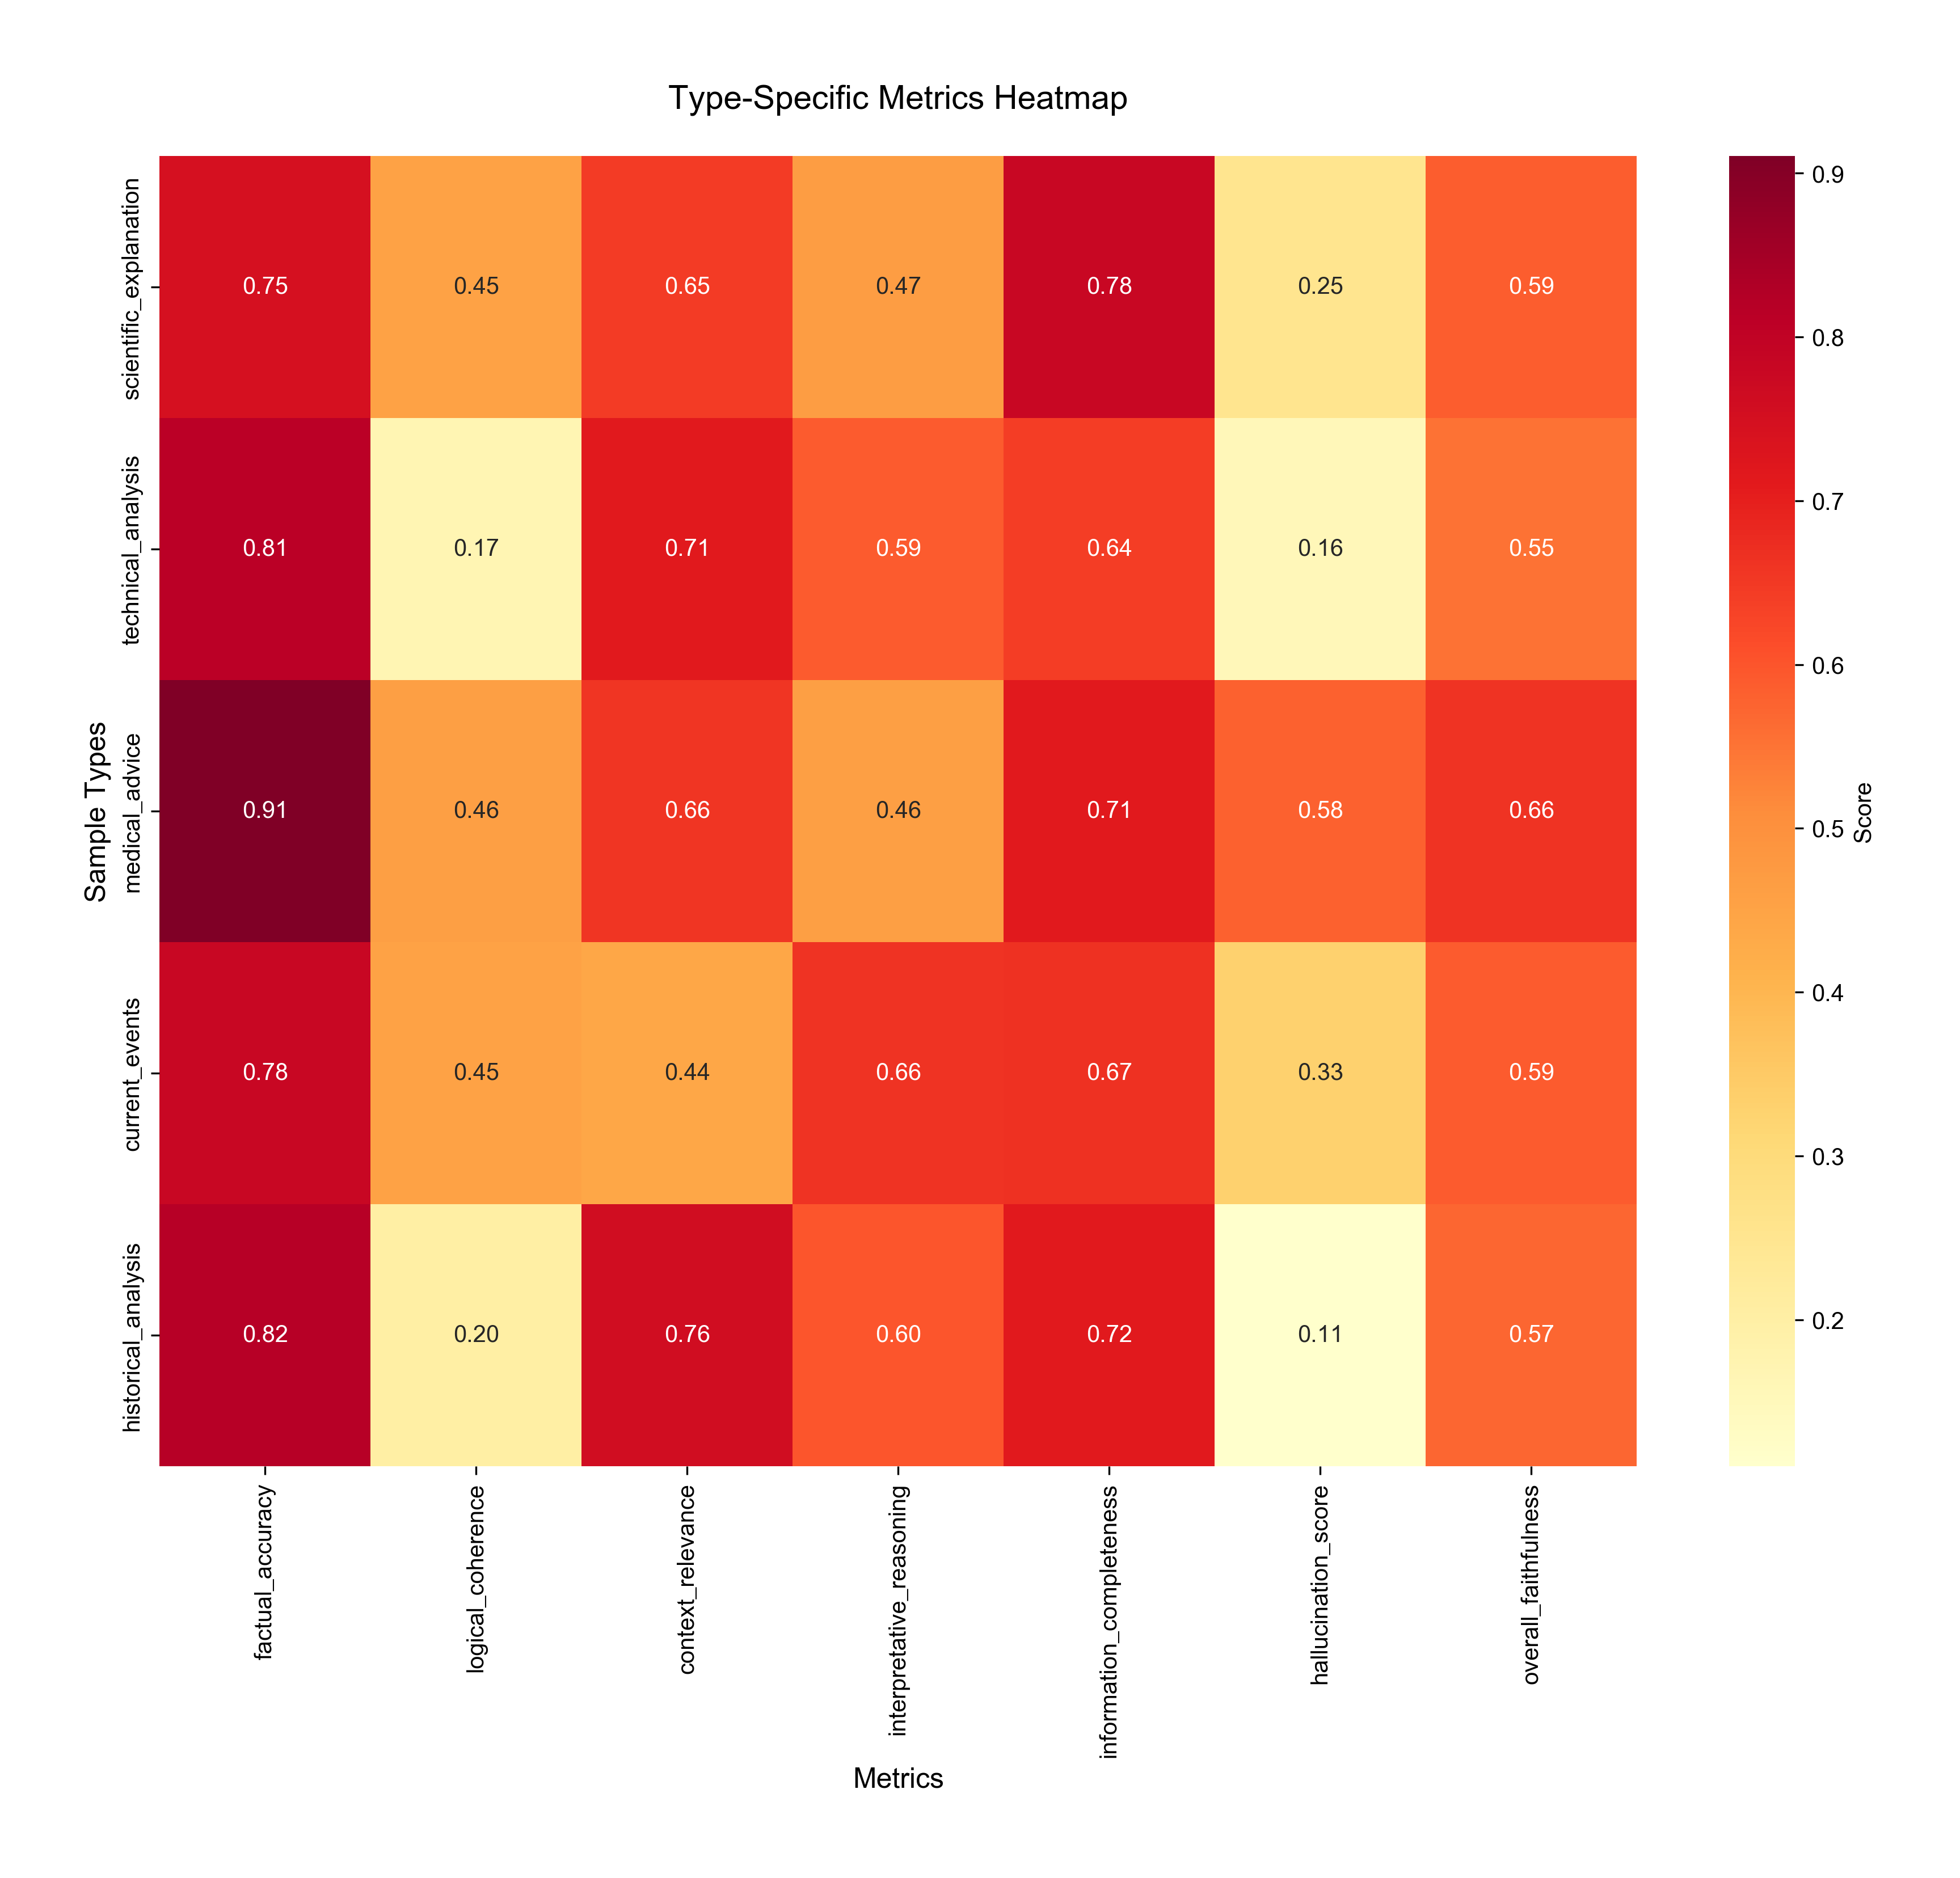
\includegraphics[width=\textwidth]{figures/visualization/metrics_heatmap_gpt-4.png}
    \caption{GPT-4}
    \label{fig:metrics_heatmap_gpt4}
\end{subfigure}
\caption{Metric Correlation Heatmaps by Model}
\label{fig:metrics_heatmaps}
\end{figure}

\textbf{Key Correlations}:
\begin{itemize}
    \item Strong positive correlation between factual accuracy and information completeness
    \item Negative correlation between hallucination scores and logical coherence
    \item Moderate correlation between context relevance and interpretative reasoning
\end{itemize}

\subsubsection{Metric Composition Analysis}
The stacked bar analysis illustrates the relative contribution of each metric to the overall faithfulness score.

\begin{figure}[!htbp]
\centering
\begin{subfigure}[b]{0.32\textwidth}
    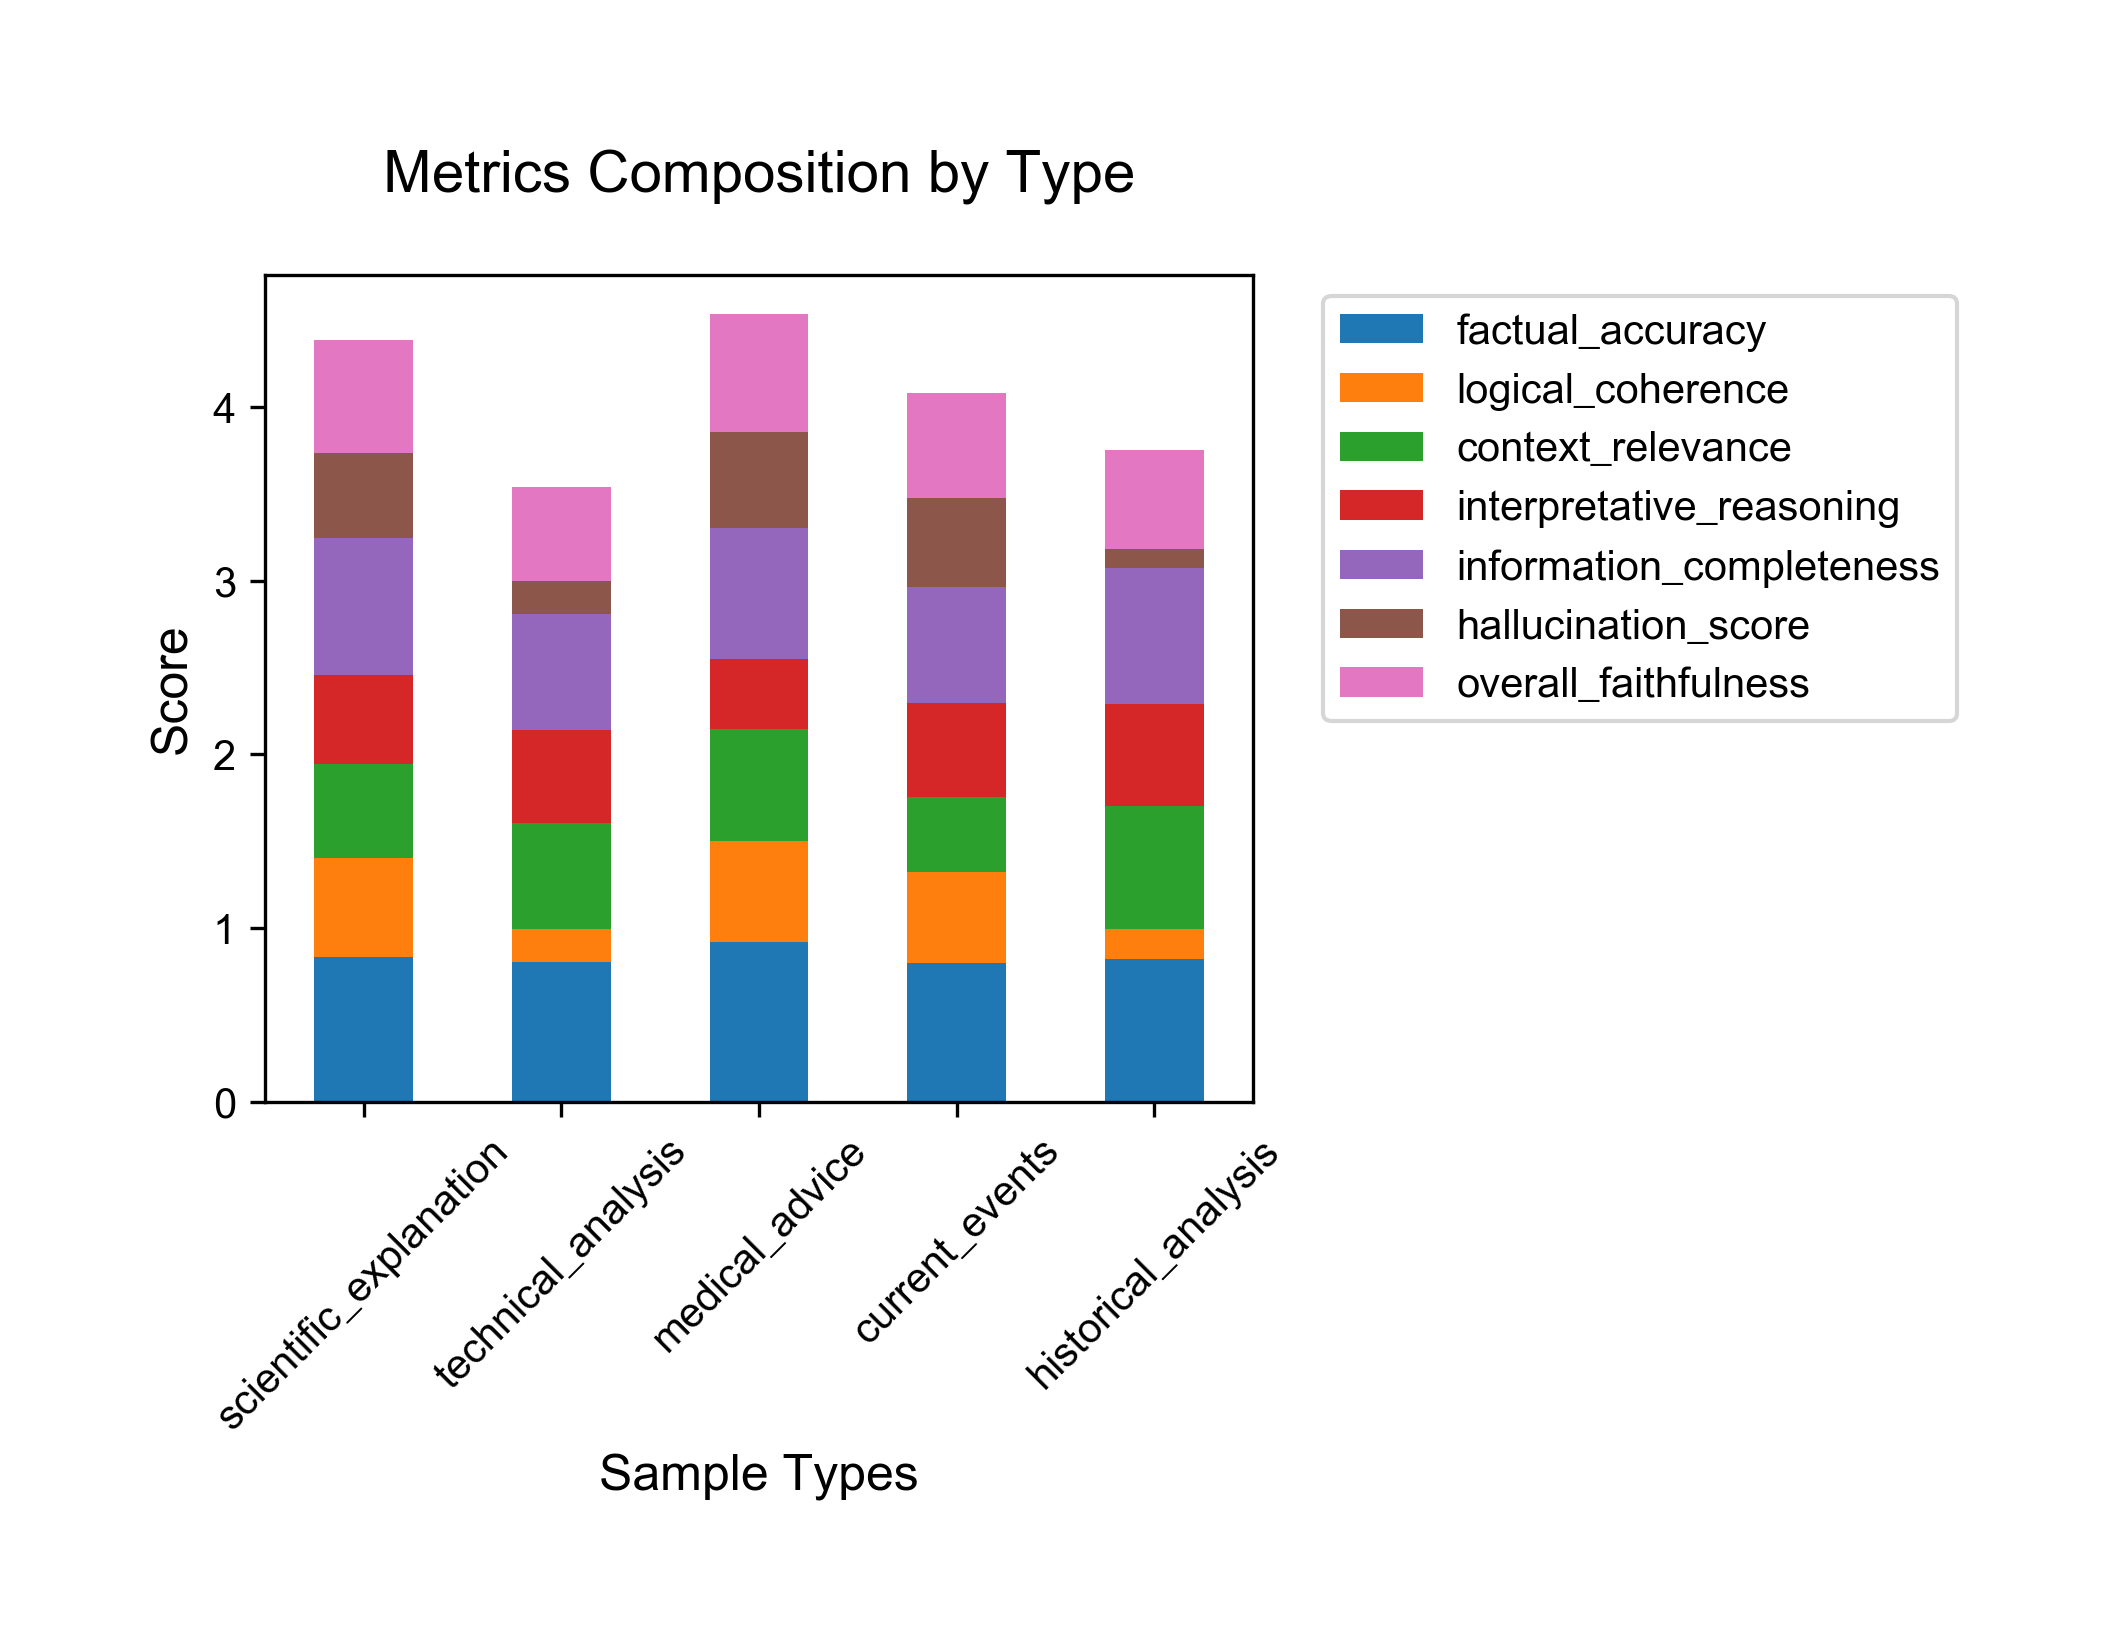
\includegraphics[width=\textwidth]{figures/visualization/metrics_stacked_bar_gpt-3.5-turbo.png}
    \caption{GPT-3.5-Turbo Composition}
    \label{fig:metrics_stacked_bar_gpt35}
\end{subfigure}
\hfill
\begin{subfigure}[b]{0.32\textwidth}
    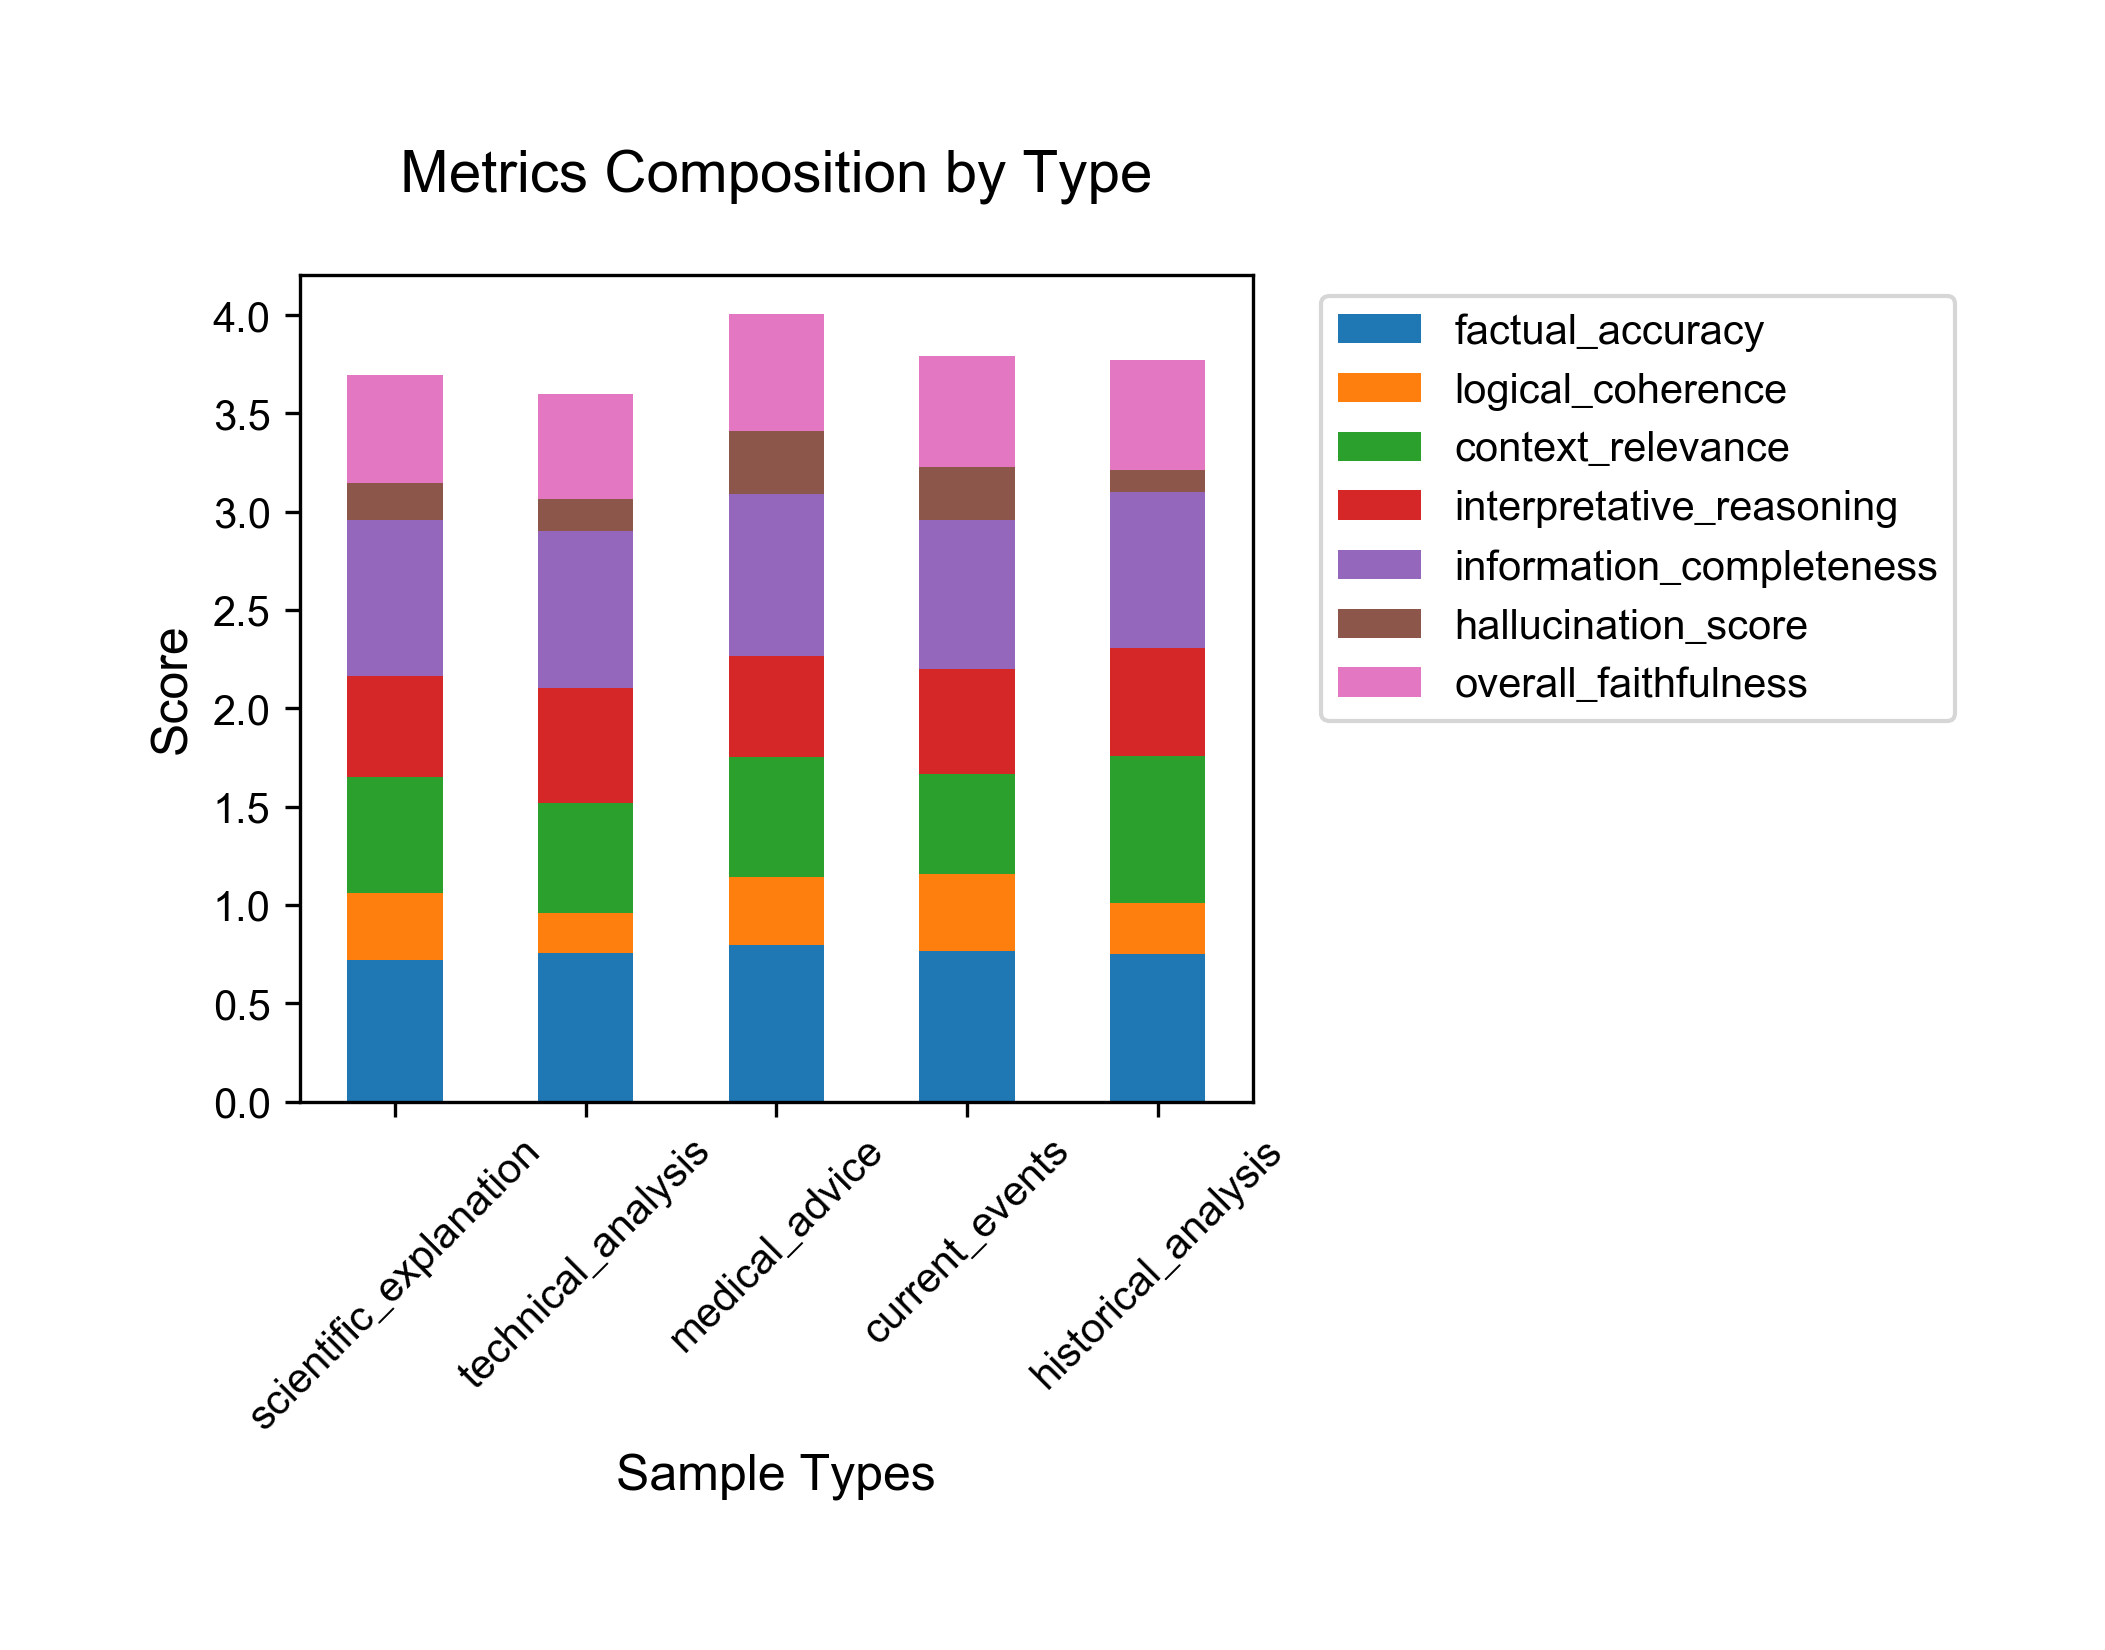
\includegraphics[width=\textwidth]{figures/visualization/metrics_stacked_bar_gpt-4-turbo.png}
    \caption{GPT-4-Turbo Composition}
    \label{fig:metrics_stacked_bar_gpt4t}
\end{subfigure}
\hfill
\begin{subfigure}[b]{0.32\textwidth}
    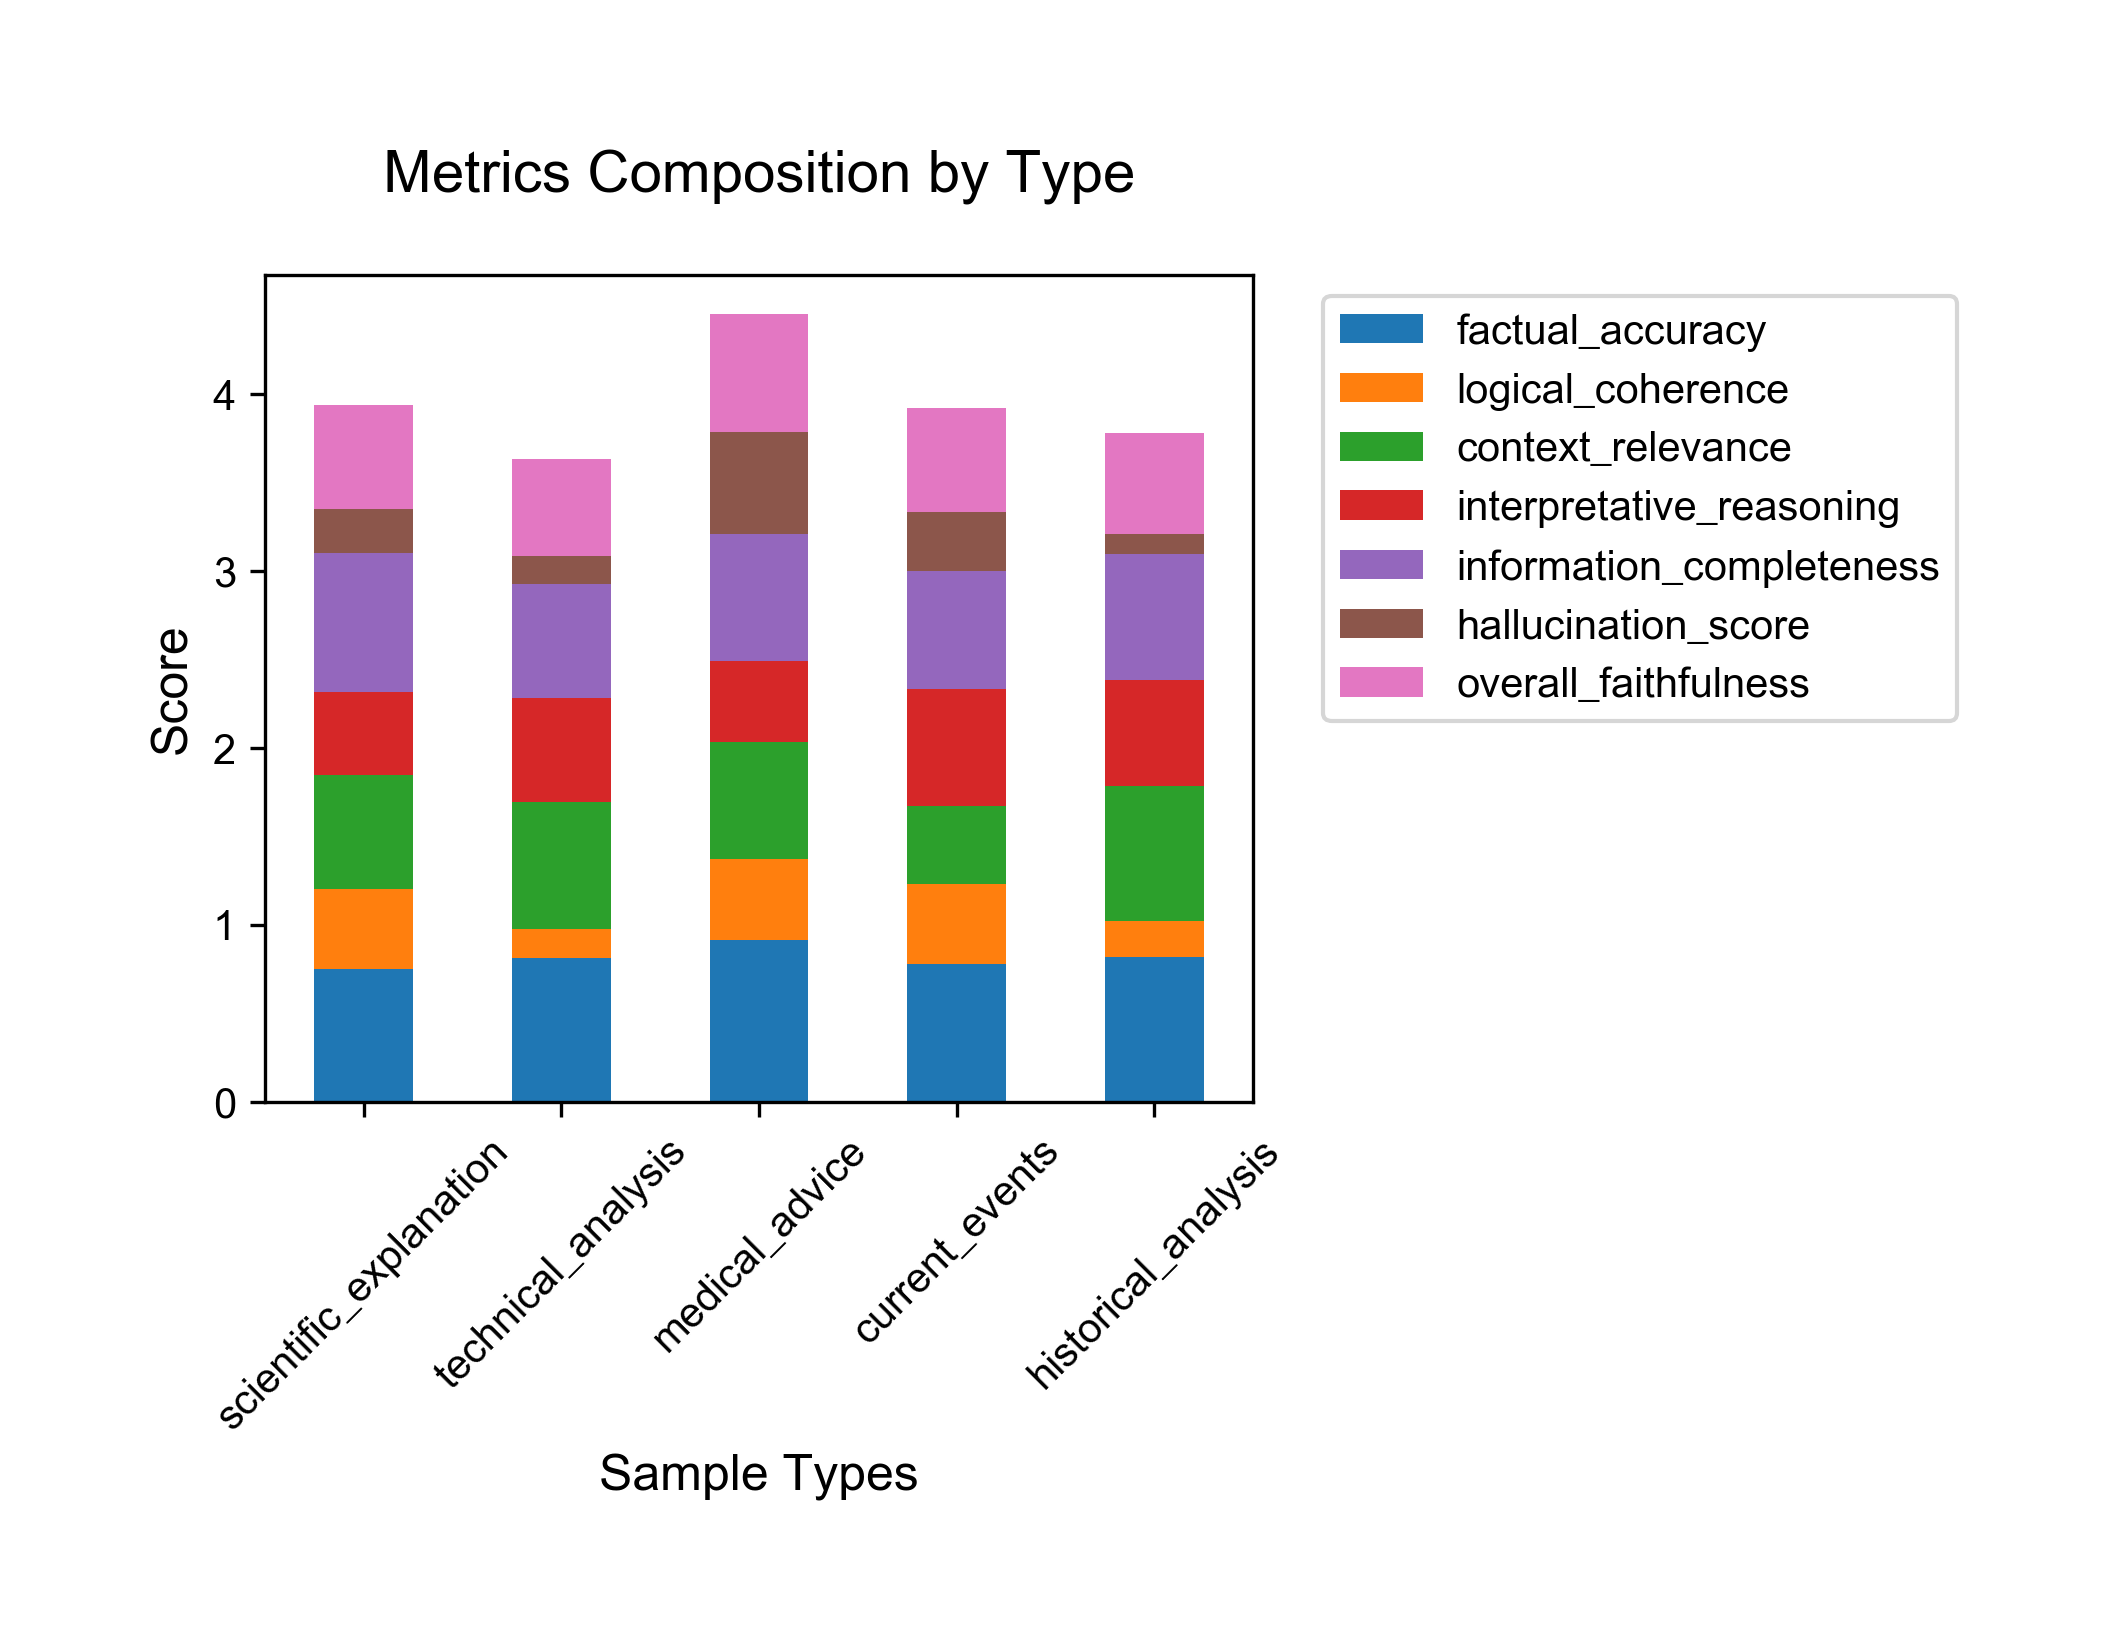
\includegraphics[width=\textwidth]{figures/visualization/metrics_stacked_bar_gpt-4.png}
    \caption{GPT-4 Composition}
    \label{fig:metrics_stacked_bar_gpt4}
\end{subfigure}
\caption{Metric Composition Analysis by Model}
\label{fig:metrics_stacked_bars}
\end{figure}

\textbf{Composition Insights}:
\begin{itemize}
    \item Factual accuracy contributes the largest proportion to overall faithfulness
    \item Information completeness shows consistent contribution across models
    \item Hallucination scores have varying impact on different models
\end{itemize}

\subsection{Performance Patterns}

\subsubsection{Model-Specific Patterns}
\begin{itemize}
    \item \textbf{GPT-3.5-Turbo}:
    \begin{itemize}
        \item Excels in factual accuracy and information completeness
        \item Shows consistent performance across different sample types
        \item Higher hallucination scores indicate potential for improvement
    \end{itemize}
    
    \item \textbf{GPT-4-Turbo}:
    \begin{itemize}
        \item Strong in information completeness and context relevance
        \item Lower logical coherence scores suggest areas for enhancement
        \item Most effective at minimizing hallucinations
    \end{itemize}
    
    \item \textbf{GPT-4}:
    \begin{itemize}
        \item Balanced performance across all metrics
        \item Superior context relevance and interpretative reasoning
        \item Moderate hallucination control
    \end{itemize}
\end{itemize}

\subsubsection{Type-Specific Patterns}
\begin{itemize}
    \item \textbf{Scientific Content}:
    \begin{itemize}
        \item High factual accuracy across all models
        \item Challenges in maintaining logical coherence
        \item Variable hallucination control
    \end{itemize}
    
    \item \textbf{Technical Content}:
    \begin{itemize}
        \item Strong context relevance
        \item Lower logical coherence scores
        \item Effective hallucination control
    \end{itemize}
    
    \item \textbf{Medical Content}:
    \begin{itemize}
        \item Highest factual accuracy scores
        \item Strong information completeness
        \item Variable hallucination control
    \end{itemize}
\end{itemize}
